\chapter{Methods of data structuring}
\label{ch:methods}

% This chapter contains a comprehensive survey of methods that
% are used to store and structure data in the wild.

% ACHTUNG: Nur das jeweils charachteristische sollte beschrieben werden
% Beschränkung aufs Wesentliche, Extremfälle, Besonderheiten
% Deutlich machen: Warum ist diese Typologie/Classification sinnvoll

This chapter holds the main empirical part of my thesis. Based on intensive
review of literature and standards, I give a comprehensive analysis of methods
and systems for structuring and describing data. The summary focuses on
conceptual properties: details of implementation such as performance and
security, are only mentioned briefly, if they show why specific techniques have
evolved. The goal of this analysis is to later find patterns and paradigms
independent from particular methods. For this reason I followed
\textcite{Meek1995} whose trick to become language-independent was ``to develop
a healthy disrespect for all languages, and look for faults in them all the
time.'' The division of methods in sections partly anticipates a more detailed
typology that will be developed in detail in chapter~\ref{ch:findings}. The
survey starts with character encodings (section~\ref{sec:characters}) that are
needed to express any textual data.  Identifiers
(section~\ref{sec:identifiers}) are used as part of all other methods as as
well. The most basic method to store and manage digital data are files
(section~\ref{sec:filesystems}) followed by databases
(section~\ref{sec:databases}). The analysis does not consider concrete database
systems, but general database models which \tacro[Database Management
System]{Database Management Systems}{DBMS} can be classified into.  Data
structuring or serialization languages (section~\ref{sec:dsl}) organize data in
general forms for storage and exchange; popular examples include \acro{XML},
\acro{CSV}, and \acro{RDF}. There is some overlap with markup languages
(section~\ref{sec:markuplanguages}), which mainly apply to text and similar
sequential data. Schema languages (section~\ref{sec:schemas}) express logical
schemas as data formats.  Conceptual modeling languages (\ref{sec:modelangs})
are used to capture a part of reality in formal language. They are often
combined with a graphical notation which is a strict form of a conceptual
diagram (section~\ref{sec:diagrams}).  Query languages
(section~\ref{sec:queries}) can define or be part of an \tacro{Application
programming Interface}{API} to select or identify a specific piece of data.

\pagebreak
\section{Character and number encodings}
\label{sec:characters}

\begin{quotation}%
\verb|Breakdowns : portrait of the artist as a young %@[squiggle][star]!| \\
\quotationsource
Unknown library cataloger, titling a book by \Person[Art]{Spiegelman}
\end{quotation}

% Breakdowns : Portrait des Künstlers als junger %@[Schnörkel][Stern]!
% Kommentar: In der Vorlage "Schnörkel" und "Stern" als Symbol wiedergegeben

\noindent All data must be written down in some form. At least a standardized
set of base symbols (\Term{character}s) is needed together with a set of
conventions how to meaningfully combine these symbols. We call this two sets a
\Term{writing system} or \term{notation}.  The connection of data and writing
systems is not an invention of the digital age: Cuneiform script on clay
tablets, the earliest known records of a writing system from the 4th millennium
BC, was first used exclusively for accounting and record keeping, thus for
capturing data.  The simplest writing system can only write down sequences of
binary data. It consists of two distinct symbols (usually called zero and one),
and the convention of concatenating these symbols to sequences. More complex
writing systems involve more characters. A \Term{character encoding} maps
characters and their combination rules to a writing system on symbols that can
easier be stored and communicated. Examples of character encodings include
Morse code, Braille, the \tacro{American Standard Code for Information
Interchange}{ASCII}, and \term{Unicode}. Digital character encodings map
characters to a sequence of bits. Before Unicode became the dominant character
encoding standard (starting in the early 1990s), there were many alternative
encodings for different sets of characters. Table~\ref{tab:aringencodings}
lists some pre-Unicode encodings and their mappings of the capital letter
\r{A}:

\begin{table}[h]
\centering
\begin{tabular}{l|r|r}
 \textbf{encoding} & \textbf{hexadecimal} & \textbf{binary} \\
\hline
 US-ASCII           & --- & --- \\
\hline
 ISO~646 DK/NO/SE   & \verb|5D| & \verb| 1011101| \\
\hline
 EBCDIC CP37 etc.   & \verb|67| & \verb|01100111| \\
\hline
 Mac~OS~Roman       & \verb|81| & \verb|10000001| \\
\hline
 Allegro-DOS/IBM437 & \verb|8F| & \verb|10001111| \\
\hline
 NeXTSTEP           & \verb|86| & \verb|10000110| \\
\hline
 ISO 8859-1         & \verb|C5| & \verb|11000101| \\
\hline
 ANSEL (MARC-8) combining \r{} + A & \verb|EA 41| 
  & \verb|11101010 01000001| \\
\end{tabular}
\caption{Various character encodings of the capital letter \r{A}}
\label{tab:aringencodings}
\end{table}

\subsection{Unicode}
\label{sec:Unicode}

Unicode aims at unifying all binary character encodings by covering all
characters for all writing systems of the world, modern and ancient
\cite{Unicode6}. The standard includes graphemes and grapheme-like units like
punctuations, technical symbols, and many other characters used in writing
text. The Unicode standard defines a \Term{grapheme} as ``a minimally
distinctive unit of writing in the context of a particular writing system.'' or
``what a user thinks of as a character''.  For instance the lines in
example~\ref{ex:loremipsum} consist of equal sequences of graphemes in Unicode
because typographic differences do not matter.

\begin{example}
\centering
\includegraphics[width=3cm]{img/loremipsum.jpg}
\caption{Equal sequences of graphemes (if encoded in Unicode) }
\label{ex:loremipsum}
\end{example}

In contrast to earlier systems, Unicode also covers multiple combination
rules, such as combining diacritics, bidirectional text, line and paragraph
separators etc. Unicode even included language tags --- special characters to
identify text as belonging to a particular language --- but this practice has
been marked as deprecated in favor of \term{markup language}s. The following
analysis of character encodings focuses on Unicode. It is referenced in many
other standards, and most characters of any other other relevant digital
character encoding are also located at some place in Unicode. Unicode is
explicitly designed as open, evolving standard.  New versions do not remove or
change characters, but only add new characters and possibly change character
properties after careful deliberation. That explicitly makes any possible
abstract character a potential candidate for inclusion in the Unicode standard.
To do so, one can define character mappings in private use areas, but there is
no standard way to tell external applications about appearance and other
properties of the corresponding graphemes. For this reason the use of Unicode
is limited to symbols that are officially accepted as graphems in the standard
--- for instance \term{written sign language} \cite{Sutton2002} and other
two-dimensional notations are not included.  The set of characters encoded in
Unicode is called the \Tacro{Universal character set}{UCS} and the set of
symbols, which is a subset of the integer values, is called the \Term{Unicode
code point}s (\format{codepoint}) in table~\ref{tab:unicode}).  All Unicode
code points are located in the range \Ox{00} to \Ox{10FFFF} which theoretically
makes 1,114,112 possible values, expressible in 21 bit. A Unicode code points
is referred to in documentation by writing `\U{}' before its value in
hexadecimal notation. By now, most code points are not assigned\footnote{As of
Unicode~6.0.0 there are 109,449 assigned graphical characters, 207 special
purpose characters for control and formatting, and 142,999 reserved for private
use.} and 2,114 values are explicitly excluded: the \term{surrogates} \U{D800}
to \U{DFFF} and 66 special \format{noncharacter} codes  are permanently
reserved for internal use. They are forbidden for use as character code point
in \acro{UCS} and in open interchange of Unicode text data
(table~\ref{tab:unicode}).

% surrogates: %\cite[section 16.6]{Unicode6} 
% noncharacters: %\cite[section 16.7]{Unicode6}

\begin{table}[ht]
\begin{lstlisting}[language=BNF]
 codepoint    = [#x00-#x10FFFF]
 surrogate    = [#xD800-#xDFFF]
 ustring      = ( codepoint - surrogate )*
 noncharacter = [#xFDD0-#xFDEF] | #xFFFE |#xFFFF |#x1FFFE|#x1FFFF|
  #x2FFFE|#x2FFFF|#x3FFFE|#x3FFFF|#x4FFFE|#x4FFFF|#x5FFFE|#x5FFFF| 
  #x6FFFE|#x6FFFF|#x7FFFE|#x7FFFF|#x8FFFE|#x8FFFF|#x9FFFE|#x9FFFF| 
  #xAFFFE|#xAFFFF|#xBFFFE|#xBFFFF|#xCFFFE|#xCFFFF|#xDFFFE|#xDFFFF|
  #xEFFFE|#xEFFFF|#xFFFFE|#xFFFFF|#x10FFFE|#x10FFFF
\end{lstlisting}
\caption{Symbol ranges in Unicode}
\label{tab:unicode}
\end{table}

Unicode characters are not directly mapped to binary sequences. Instead the
standard defines a number of encodings such as UTF-8, UTF-16 etc. to map
\format{ustring} to sequences of Bytes. The mapping is neither injective, nor
surjective or functional. Table~\ref{tab:utfaringencodings} lists several
schemes that all encode the capital letter \r{A}. The abbreviations `LE' and
`BE' indicate the byte order little-endian (default) and big-endian.  Different
combinations of UTF-8, UTF-16, UTF-32, or UTF-EBCDIC\footnote{UTF-EBCDIC was
defined to better support mainframe EBCDIC computers, which nowadays may only
be found in archaic systems, like nuclear power plants.} with BE or LE define
alternative transformation formats.  They can easily be mapped to each other as
isomomorphic encodings of \acro{UCS}. A full breakdown of the encoding of the
composed character is provided with example~\ref{ex:Aring} in
section~\ref{sec:levels}.

% on UTF-8
% http://www.cl.cam.ac.uk/~mgk25/ucs/utf-8-history.txt
% created by Ken Thompson

\begin{table}[h]
\centering
\begin{tabular}{l|r|r}
 \textbf{Unicode encoding scheme} & \textbf{hexadecimal} & \textbf{binary} \\
\hline
 UTF-16, LE: \r{A}ngstr\"{o}m sign & \verb|21 2B| 
& \verb|00100001 00101011| \\
\hline
 UTF-16, BE: \r{A}ngstr\"{o}m sign & \verb|2B 21|
& \verb|00101011 00100001| \\
\hline
 UTF-16, LE: \r{A} & \verb|00 C5|
& \verb|00000000 11000101| \\
\hline
 UTF-8, LE: \r{A} & \verb|C3 85|
& \verb|11000011 10000101| \\
\hline
 UTF-16, LE: A + combining \r{} & \verb|00 41 03 0A| 
& \verb|00000000 01000001| \\
& & \verb|00000011 00001010| \\
\hline
 UTF-8, LE: A + combining \r{} & \verb|41 CC 8A| 
& \verb|01000001 11001100| \\ & &  \verb|10001010| \\
\end{tabular}
\caption{Various Unicode encoding schemes encoding the capital letter \r{A}}
\label{tab:utfaringencodings}
\end{table}

As described by \textcite{Davis2010}, Unicode does not directly encode
characters in UCS but it encodes graphemes, which may be combined to grapheme
clusters as user-perceived characters. In general each graphem should be
assigned to exactly one Unicode code point. For historical reasons there are
some exceptions, like \U{00C5} (latin capital letter a with ring above) and
\U{212B} (angstrom sign). One may argue that both are different characters, if
used in different context, but as they both map to the same visible grapheme,
the difference is difficult to sustain. Some same grapheme clusters can be
created by multiple sequences of codepoints. For this reason the Unicode
standard defines two kinds of equivalence between code point sequences:
\Term[canonical equivalence (Unicode)]{canonical equivalence} and
\Term[compatible equivalence (Unicode)]{compatible equivalence}. Canonical
equivalence is based on \term[character (de)composition]{character
composition}, that is the process of combining multiple characters to one ---
the reverse process is called decomposition. A combined character sequence and
its canonical equivalent precomposed character should always have the same
visual appearance and behaviour. Compatible equivalence is based on minor
visual differences, that may be significant in some contexts only. Examples of
compatible equivalences are font variants, ligatures, and digraphs.
Composition and decomposition are mappings that ground on character properties
of the Unicode character database. Given these mappings, there are four
official \term{normalization} forms \cite{David2009}: %
\url{http://unicode.org/reports/tr15/} \tacro{Normalization Form D}{NFD}
transforms a string by mapping each character to its canonical decomposition.
\tacro{Normalization Form C}{NFC} first decomposes all characters with
\acro{NFD} and then transforms the resulting string by canonical composition.
For instance a string that contains the letter \r{A} in any of the forms
\U{212B}, \U{C5}, and \U{41} followed by \U{038A} will only contain it as
\U{C5} after \acro{NFC}.  \tacro{Normalization Form KD}{NFKD} transforms a
string by compatible decomposition and \tacro{Normalization Form KC}{NFKC} adds
canonical (sic!) composition after compatible decomposition. \acro{NFKD}
subsumes \acro{NFD} and \acro{NFKC} subsumes \acro{NFC}.  Normalization also
provides a unique order for combining marks, so it can be used to determine
string equivalence. Once normalized, a string should not change when normalized
again with the same operation.\footnote{This implies that equivalence mappings
of a given character cannot be changed in future versions of Unicode. The
stability guarantee on normalization only applies to assigned characters in
\acro{UCS}.} None of the normalization forms is bijective (fully reversible)
because each maps the set \format{ustring} to a smaller subset.

On a closer look, Unicode contains many inconsistencies and exceptions in
respect to character properties and normalization. For example Chinese
characters are composed of strokes, but there is no decomposition mapping
to the set of strokes which form a given chinese character. Some icons,
ligatures and digraphs are included in \acro{UCS} but others are rejected,
even if used as distinct graphemes.\footnote{For instance one method of writing
the M\=aori language in the early 20th century contained a special `wh' ligature
as distinct character. Although there are printed books that use this letter,
it was rejected for inclusion in Unicode. See 
\url{http://unicode.org/faq/ligature_digraph.html} for the objections of 
Unicode Consortium in ligatures and digraphs. Icons and pictograms are
reluctantly included as well, but Unicode version 6.0 introduced
several hundred Emoji icons for animals, clothes, vehicles, food and other
random artifacts. The history including the capital sharp s, rejected in
2004 but included as \U{1E9E} in Unicode version 5.1.0 after a second
proposal, reveals some interesting insight into the process of standardization.}
Said that, one must keep in mind that the aim of Unicode is not to create an
objective model of all human writing systems but to ensure compatibility in
exchange of character strings. In addition to composition properties, the
character database contains a large number of attributes to describe
relevant characteristics and relations like character type, case, order
etc. \cite{Whistler2008}. However this metadata is relatively static and
excludes many aspects like historical relations and visual similarities.
Based on character properties, applications can define custom
normalization forms, for instance \acro{NFKD} followed by
lowercase case-folding and removal of all diacritics.

While Unicode is the dominant standard for character encoding on the level of
byte sequences, there are other methods that express characters as sequences
of other characters or symbols (see table~\ref{tab:otheraringencodings}).
Some encodings are not reversible because they map multiple characters to the
same symbols. Problems frequently arise, if data include symbols without known
character encoding or if different creators and users of data do not agree on
a common character encoding and interpretation.

\begin{table}[h]
\centering
\begin{tabular}{l|l}
 \textbf{encoding} & \textbf{symbols} \\
\hline
 named HTML entity & \verb|&Aring;| \\
\hline
 XML character entity & \verb|&#xc5;|, \verb|&#xC5;|, \verb|&#197;|,
\verb|A&#x030A;| \ldots \\
\hline
 Swedish 6 dot Braille & 
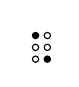
\begin{tikzpicture}[baseline]
   \path[use as bounding box] (-1mm,0) (2mm,0) (2mm,4mm);
   \draw ( 0, 0) circle (.4mm);
   \draw ( 0,.15) circle (.4mm);
   \draw[fill] ( 0,.30) circle (.4mm);
   \draw[fill] (.15, 0) circle (.4mm);
   \draw (.15,.15) circle (.4mm);
   \draw (.15,.30) circle (.4mm);
 \end{tikzpicture} 
~pattern P16 (Unicode \U{2821})
\\ \hline
Eurobraille 8 dot&
 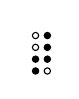
\begin{tikzpicture}[baseline]
   \path[use as bounding box] (-1mm,0) (2mm,0) (2mm,5.5mm);
   \draw[fill] ( 0, 0) circle (.4mm);
   \draw[fill] ( 0,.15) circle (.4mm);
   \draw ( 0,.30) circle (.4mm);
   \draw ( 0,.45) circle (.4mm);
   \draw (.15, 0) circle (.4mm);
   \draw[fill] (.15,.15) circle (.4mm);
   \draw[fill] (.15,.30) circle (.4mm);
   \draw[fill] (.15,.45) circle (.4mm);
 \end{tikzpicture} 
~pattern P34567 (Unicode \U{287C})
\\ \hline
Transcription & Aa
\\ \hline
Morse code (\r{a} = \`{a}, no case) & $\cdot$ - - $\cdot$ - \\
\end{tabular}
\caption{Additional character encodings of \r{A}}
\label{tab:otheraringencodings}
\end{table}

% Some sources:
% NeXT
%  http://unicode.org/Public/MAPPINGS/VENDORS/NEXT/NEXTSTEP.TXT
% IBM EBCDIC
%  http://www.unicode.org/Public/MAPPINGS/VENDORS/MICSFT/EBCDIC/CP037.TXT
%
% ANSEL: combining ring above (EA) + A (41)
% US-ASCII, ISO~646 (7-bit with national variants)
% ISO~8859 (8-bit)

% (see \cite{Whistler2008} \url{http://unicode.org/reports/tr23/} for 
% a metamodel of Unicode properties).

\subsection{Number encodings}
\label{sec:numberencodings}

A typical misconception about computers is that they deal with numbers, but
they only deal with bits.  Sequences of bits are used to encode numbers, just
like character encodings encode characters. In contrast to arbitrary
characters, the \term{value space} of numbers includes a mathematical model,
that defines algebraic operations for calculation (see
section~\ref{sec:datatypes}).  Digital number encodings should support these
operations on representations of numbers, but they are typically defined on a
limited computational model. First of all, most number systems are infinite
while most number encodings limit each number to a fixed number of bits. The
most prominent types of number encodings are integers, floating point numbers,
and possibly boolean data types which map one bit to one boolean value (true or
false).

\Term{Integer} data types represent (a subset of) the integer numbers
$\mathbb{Z}=\set{\ldots-2,-1,0,1\ldots}$. One can encode $\mathbb{Z}$ (up to
limits of memory) by using a variable size encoding like used for instance in
the Protocol Buffers data binding language \cite{Varda2008}.  In practice most
integer data types have some fixed size of $n$ bits that store an integer value
in binary numeral system.  The range that can be encoded with $n$ bit is
$-2^{n-1}$ to $2^{n-1}-1$ for signed integers ($\format{Int}_{n}$) and $0$ to
$2^n-1$ for unsigned integers ($\format{UInt}_{n}$).

There are several encodings for subsets of the real numbers $\mathbb{R}$ with
\Term{floating point} data types as most common method.  The basic idea of
floating point numbers is to represent a real number $r$ as the result $r = m
\cdot b^x$ with two integer components, exponent $x \in \mathbb{Z}$, and
mantissa $m \in \mathbb{Z}$, and a base $b$. For example with base $b=10$ the
number $374.2$ could be represented as $3742 \cdot 10^{-1}$. The mapping allows
for multiple encodings of the same number, for instance $374.2$ is also $37420
\cdot 10^{-2}$. For this reason floating point numbers are typically stored in
normalized form where the mantissa must be in a specific range. In digital encoding, 
the base of most floating point encodings is $b=2$. The exponent is typically 
stored as unsigned integer with a fixed bias value and one can save the first bit 
of the mantissa by assuming that it must always be $1$ for normalized numbers.
Calculation with floating point numbers is tricky because there are several ways
in which the result of a calculation may not be part of the selected subset of 
$\mathbb{R}$. This can also happen in integer encodings but floating point 
encodings often support special values for this cases, such as signed zeroes 
($-0$ and $+0$ are encoded as different values), infinities ($+\inf$ and $-\inf$ 
are allowed), and ``not a number'' values (NaN). IEEE~754 \cite{ieee2008}, the
most popular floating point encoding, distinguishes between two kinds of NaN, 
quiet NaN and signaling NaN. However, there is no portable way to assign the second
as data value because either it is converted to a quiet NaN or an exception is 
raised. Furthermore IEEE~754 and related standards still allow for some variations 
in implementations that can led to different results, depending on the computer
platform \cite{Monniaux2008}.\footnote{Under specific circumstances a floating
point variable may even change its encoding without an assignment to it.}
In summary one must take care which specific floating encoding one deals with or
better avoid floating point values in favor of other encodings like
decimal notation with arbitrary precision or symbolic notation.


\section{Identifiers}
\label{sec:identifiers}

\begin{quotation}%
What's in a name? that which we call a rose by any other name would smell as sweet.\\
\quotationsource{\Person[William]{Shakespeare}: Romeo and Juliet}
\end{quotation}

% Identifiers are used throughout all other encoding methods. They are used to
% solve the problem of identification in a very limited context. In a broader
% context this problem is much harder to tackle as shown in
% section~\ref{sec:identityandequality}.

\noindent While character and number encodings are used as base of data
structuring, \term{identifier}s virtually pervade systems to structure and
describe data on all levels. This section first introduces basic identifier
principles (section~\ref{sec:idbasics}) followed by properties of namespaces and
qualifiers (section~\ref{sec:qualifiers}) which identify the context of
association between identifier and referred thing. Identifier systems
(section~\ref{sec:idsystems}) provide an infrastructure in which identifiers are
assigned, managed, and used. Part~\ref{sec:descrids} on descriptive identifiers
and section~\ref{sec:orderedids} on ordered identifiers highlight two important
but often overlooked properties of identifiers on a more theoretical level.
Finally hash codes as special kind of distributed identifier systems are
explained in section~\ref{sec:hashes}. A summarized overview of designated
identifier properties is given in table~\ref{tab:idprops}.

\subsection{Basic principles}
\label{sec:idbasics}

In its most general form, a digital identifier is a piece of data (string,
number, letter, symbol, etc.) that refers to an object. This makes
identifiers a special type of metadata which more generally describe objects.
In contrast to general metadata, an identifier should be unique (no homonyms), 
persistent and short, at least in some context. Distinct objects must have 
distinct identifiers to avoid ambiguity, and the number of identifiers that 
refer to the same object (synonyms) should be low for practical reasons. The 
following analysis is limited to digital identifiers in their general form as 
finite sequences of characters. Examples of identifiers from the previous 
section include number encodings that refer to the mathematical concepts of 
numbers, byte sequences that refer to Unicode code points, and Unicode code 
points that refer to characters. It is shown that this forms -- also known as
names, labels, locators, codes, or pointers -- only make the visible part of
an identifier. The concluding example of Pica format field identifiers will 
then illustrate some basic properties of data identifiers. 

Most literature on identifiers deals with selected types of identifiers
or with special aspects, such as identifier persistence. More general 
discussions are provided by 
\textcite{Eriksson2010}, % Rethinking the Meaning of Identifiers in...
\textcite{Campbell2007} % Identifying the identifiers
\textcite{Coyle2006}, 
\textcite{Vitiello2004}, 
\textcite{Lynch1997},
and \textcite{Kent1991}. The authors define identifiers as data objects that
``refer to'', ``reference'', ``represent'', or ``serve as surrogate for'' 
other objects, but the general idea is the same: a relatively short
piece of data is associated with another (data) object. 
\textcite{Campbell2007} 
provides a more detailed deconstructions of identifiers in six parts:

\begin{enumerate}
\item a ``thing'' that is referenced
\item a ``symbol'' that references the thing. Unless otherwise indicated,
  this symbol in particular is meant by the word ``identifier''
\item an ``association'' between the symbol and the thing
\item a ``context'' that the association occurs within
\item an ``agent'' that states the association and context
\item a ``record'' of the association, context, and ideally also the agent
\end{enumerate}

In the following the same terminology will be used. Symbol, thing, and
association are typically found as ``symbol'', ``referent'', and ``thought'' or
under different names in the \term{semiotic triangle} \cite{Ogden1923} as
described in section~\ref{sec:semiotics}.  The important aspect for the
analysis of identifiers is that there is no direct connection between symbol
(signifier) and thing (signified).  It requires an association that always
depends on some context, is established by an agent, and may or may not be
recorded.

Following the philosophical position of radical \term{constructivism}
\cite{Glasersfeld1990}, one can even neglect the thing, as there is no direct
access to real-world objects by language. This also applies to digital
identifiers about things in the reality realm (in terms of data modeling).
However, digital identifiers about digital objects can be compared with their
referents, because both are recorded in data. In fact digital records of
identifiers and their referents are common practice in many data structures and
known as \Term[lookup table]{lookup tables}. In some cases one can even swap
symbol and referent, because both are unique on their side of the table (see
table~\ref{tab:pica3pp} for an example).

Unambiguity (each identifier must refer to only one object) and uniqueness
(for each object there should be only one identifier) of often combined as
\Term{uniqueness} as most important requirement for an identifier.
Other properties frequently cited as important qualities are \Term{persistence}
(identifiers should not change over time), \Term{scope} (the context of an
identifier should be broad or even `global'), \Term{readability} (identifiers
should be easy to remember or contain information), and \Term{actionability}
(given an identifier one should be able to do something with it,
for instance access the identified object). A summary of these and more
designated identifier properties is given in table~ \ref{tab:idprops}.
To ensure the required
properties it needs an \term{identifier system} as controlled mechanism 
or convention for creating, managing, and using identifiers 
(see part~\ref{sec:idsystems}). When we analyze general data, identifier 
properties can also indicate whether some piece of data is actually used 
as identifier or not: being an identifier is nothing inherently inscribed 
in data, but it is an example of a popular data pattern, that is used all
all over systems to structure and describe data. 

\subsectionexample{Field identifiers in PICA format}
\label{ex:picafieldids}

\begin{table}[h]
\centering
\begin{tabular}{r|l|l|l|l|l}
description & year        & title       & edition     &  place and publisher & DDC \\
\hline
Pica3 tag   & \verb|1100| & \verb|4000| & \verb|4020| & \verb|4030| & \verb|5010| \\
Pica+ tag   & \verb|011@| & \verb|021A| & \verb|032@| & \verb|033A| & \verb|045F| \\
repeatable  & no & no & no & yes & yes \\
\end{tabular}
\term*{Pica}
\caption{Some fields of Pica record format}
\label{tab:pica3pp}
\end{table}

The bibliographic record format \Term{Pica} consists of a simple 
field-subfield-structure, similar to \term{MARC} (compare with figure 
\ref{fig:marcrecord}). Each field can be identified by a so called
Pica3 tag or by a Pica+ tag. Figure~\ref{tab:pica3pp} lists a lookup table 
for some fields with their tags and a repeatability flag from the cataloging 
rules of the \acro{GBV} library network \cite{Pica2010}. 
Assuming that the
fields somehow refer to things in the reality realm, we cannot directly
map from tags to these things. Fields like ``place and publisher'' also
indicate that the referent can be quite artificial: most people know places
and maybe publishers, but what kind of ontological status has their 
combination? Beside the intangible referent of such artificial identifiers, 
textual descriptions make no good identifiers, because one can write them in
several forms (the original descriptions are given in German) and because 
there may be different fields with same description. Tags in contrast can 
at least identify field descriptions and tags of the other kind (Pica3 to 
Pica+ and vice versa), because they all exist in the data realm. The 
repeatability flag finally identifies a thing from the conceptual realm, 
namely the set of fields, that are repeatable (\verb|yes|) or not repeatable
(\verb|no|). In practice one must always take in mind, in which context an identifier 
is used. A Pica3 tag like \verb|5010| may refer to the corresponding
Pica+ flag \verb|045F|, to a concrete set of field value, or to the abstract
concept of the field. In data structuring we often deal with cascaded 
identifiers that only link to the reality realm in a last step. For instance 
\verb|045F| refers to the ``DDC'' field, which in a bibliographic records 
contains a notation from the \tacro{Dewey Decimal Classification}{DDC},
which by itself is another identifier. % TODO: see part ...


\subsection{Namespaces and qualifiers}
\label{sec:qualifiers}
% there seems to be no general literature on namespaces (!)

\Term[namespace]{Namespaces} and \Term[qualifier]{qualifiers} are both used to
avoid the problem of \term{homonymy}. In addition they can provide context and
refer to authority through a hierarchy of identifiers. A possible term to 
describe both is \Term{qualified identifier}. Qualified identifiers are used in 
formal systems like programming languages and knowledge organization systems
(thesauri, classifications, authority files etc.) where a name must always 
refer to one distinct object. A defined syntax in a formal language is needed 
to separate the namespace or qualifier part and the local part of a qualified 
identifier. Otherwise it would be ambiguous for instance whether `band-spectrum'
refers to a `band' of radio communication frequencies, or to the Australia band 
`spectrum' which formed in 1969, or whether the minus sign does not indicate
the existence of a namespace qualifier at all. Namespaces are typically 
prepended to the local identifier and qualifiers are added in parentheses
(see example~\ref{ex:contextids}). If the context is known as by definition of 
a \Term{default namespace}, one may also omit the qualifier or namespace.

\begin{example}[h]
\centering
\begin{tabular}{l|l|l|l|l}
identifier & local & qualifier & syntax & description \\
\hline
\texttt{Frankfurt/Main} & \texttt{Frankfurt} & \texttt{Main} 
 & \texttt{$L$/$Q$} & city name \\
\texttt{Dublin, Ohio} & \texttt{Dublin} & \texttt{Ohio} 
 & \texttt{$L$, $Q$} & city name \\
\texttt{US-OH} & \texttt{OH} & \texttt{US} 
 & \texttt{$Q$-$L$} & ISO 3166-2 area code \\
\texttt{std::set} & \texttt{set} & \texttt{std} 
 & \texttt{$Q$::$L$} & C++ identifier \\
\texttt{rdf:type} & \texttt{type} & \texttt{rdf} 
 & \texttt{$Q$:$L$} &  \acro{URI} reference in \acro{RDF} \\
\texttt{10.1000/182} & \texttt{1000/182} & \texttt{10} 
 & \texttt{$Q$.$L$} &  \acro{DOI} as specific Handle \\
\texttt{sgn-US} & \texttt{US} & \texttt{sgn} 
& \texttt{$Q$-$L$} &  \acro{IANA} language \& subtag\\
\end{tabular}
\caption{Qualified identifiers with local part ($L$) and qualifier ($Q$)}
\label{ex:contextids}
\end{example}

For some prefixed types of namespaces, the qualifier is not fixed, but
can be replaced by another prefix for the same namespace. For instance
\texttt{http://dx.doi.org/} and other known resolver addresses are actually 
used as prefix for the namespace of \Tacro{document object identifiers}{DOI}
but one could also use the \acro{DOI} as \Tacro{Uniform Resource 
Identifier}{URI} with prefix \texttt{info:uri/}. Another example is 
a prefixed element name in the \term{Extensible markup language} (\acro{XML}, 
see section~\ref{sec:xml}): some \acro{XML} applications ignore the prefix and
respect a locally defined namespace, some ignore the prefix, and some need both
to identify an element (see example~\ref{ex:xmlns} at page \pageref{ex:xmlns}). 
Finally, there are
systems in which a namespace is just an abbreviation that can be defined
and expanded as needed (see the \texttt{@prefix} statement from 
\term{Notation3} as described in section~\ref{sec:rdf} and 
table~\ref{tab:n3syntax}).

Qualifiers, more often than namespaces, may also encode a special meaning,
especially when they are used for syntactic indexing in knowledge organization
languages. For instance the identifier \texttt{Marx, Karl, 1818-1883} from 
the Library of Congress name authority file include the qualifier 
\texttt{1818-1883}. This qualifier specifies the years of birth and death of 
the identified person.\footnote{The first part of the identifier
(\texttt{Marx}) may also be seen as a namespace of all people's identifier 
with this surname, and the local part \texttt{Karl} signifies a given personal 
name, so in this example all parts encode some meaning if one takes person 
names as meaningful.} In other cases the primary role of a qualifier is to 
disambiguate, so one is more free to choose, for instance \texttt{Paris~(city)} 
and \texttt{Paris~(mythology)}, \texttt{Paris~(place)} and \texttt{Paris~(person)},
or just \texttt{Paris~(1)} and \texttt{Paris~(2)} for two distinct concepts. 
A general problem of meaningful qualifiers is the limitation to one aspect. 
For instance there are multiple early computers referred to as ``Mark~I''. 
One can either use their location as qualifier (\texttt{Mark~I~(Harvard)} and
\texttt{Mark~I~(Manchester)}) or their year of completion 
(\texttt{Mark~I~(1944)} and \texttt{Mark~I~(1949)}). Combining multiple
aspects quickly gets complicated, similar to nesting of multiple namespaces
in one mono-hierarchical system, as described in the next part.

Above all, namespaces and qualifiers do not solve the general problem of
identification but they only shift it to another domain, level, or authority.
Namespaces and qualifiers only draw aside avoid homonymy and provide context 
in some known identifier system and both are identifiers in their own right. 
To avoid an infinite chain of qualified identifiers one hasto start at some 
authority as root context, which is also known as the global namespace.

\subsection{Identifier Systems}
\label{sec:idsystems}
\label{sec:dns}

\begin{quotation}%
URIs don't change. People change them.\\
\quotationsource{\Person[Tim]{Berners-Lee} (\citeyear{BernersLee1998})}
\end{quotation}

\noindent
All identifiers are artificially created -- either explicit by naming
or implicit by providing a mechanism that creates identifiers. An 
\Term{identifier system} defines which identifiers exist (registry); or how
identifiers are created and managed (assignment politics); how recorded 
associations between identifier and referent can be looked up (resolving); 
which syntax rules as naming conventions apply (grammar); or which relations 
to other identifier systems exist. Popular digital identifier system covered 
as examples in the following are: \tacro{Uniform Resource Identifier}{URI}, 
its counterpart \tacro{Internationalized Resource Identifier}{IRI}, 
\tacro{Uniform Resource Locator}{URL}, \tacro{Uniform Resource Name}{URN},
\tacro{Domain Name System}{DNS}, \tacro{Internet Protocol}{IP},  
\tacro{International Standard Book Number}{ISBN}, and
\tacro{European Article Number}{EAN}. Relations between these systems, 
together with their character encodings are illustrated in 
figure~\ref{fig:idsysrel}.

\begin{figure}
\centering
\begin{tikzpicture}[line width=0.25mm]
\entity (URI) {URI}
 [edge from parent/.style=subtype,nodes=entity]
 child { node (URL) {URL} }
 child { node (URN) {URN} };
\entity[below=6mm of URN] (URNISBN) {URN-ISBN}; 
\draw[subtype] (URN) to (URNISBN);

\entity[below=6mm of URL] (IP) {IP};
\entity[left=5mm of IP] (DNS) {DNS};
\draw[dotted,->] (IP) -> (DNS);
\draw[dotted,->] (URL) -> (DNS);
\draw[dotted,->] (URL) -> (IP);
\draw[<->] (DNS) to (IP);

\limits ($(URI)!.65!(URL)$) to 
 node[constraint=exclusive] {} ($(URI)!.65!(URN)$);

\entity[above=6mm of URI] (IRI) {IRI};
\entity[right=14mm of URI] (ASCII) {US-ASCII};
\entity[above=6mm of ASCII] (UCS) {UCS};

\draw[dotted,->] (IRI) to (UCS);
\draw[dotted,->] (URI) to (ASCII);

\draw[suptype] (ASCII) to (UCS);
\entity[right=5mm of URNISBN] (ISBN) {ISBN}
 [edge from parent/.style=subtype,nodes=entity,
 sibling distance=19mm]
 child { node (ISBNa) {ISBN-13} }
 child { node (ISBNb) {ISBN-10} };
\limits ($(ISBNa)!0.35!(ISBN)$) to 
 node[constraint=exclusive] {} ($(ISBNb)!0.35!(ISBN)$);
\draw[<->] (ISBNa) to (ISBNb);

\entity[left=7mm of ISBNa] (EAN) {EAN};
\draw[subtype] (EAN) to (ISBNa);

\draw[<->] (ISBN) to (URNISBN);
\draw[<->] (IRI) to (URI);

%\draw[dotted,->] (ISBN) -> (ASCII);
\begin{scope}[xshift=48mm,yshift=-12mm]
\draw[dotted,->] (-6mm,2mm) to (-1mm,2mm);
\node[anchor=west] at (0,2mm) {depends on};

\draw[subtype,->] (-6mm,-5mm) to (-1mm,-5mm);
\node[anchor=west] at (0,-5mm) {subset of};

\node[constraint=exclusive] at (-3mm,-11mm) {};
\node[anchor=west] at (0,-11mm) {exclusion};

\draw[<->] (-6mm,-18mm) to (-1mm,-18mm);
\node[anchor=west] at (0,-18mm) {(partial) mapping};
\end{scope}
\end{tikzpicture}
\caption{Relations between several identifier systems}
\label{fig:idsysrel}
\end{figure}

In general any sequence of bits or other digital symbols can act as 
digital identifier. To define a possible set of sequences, an identifier system 
includes a formal language (see~\ref{sec:formallanguages})
as identifier syntax (see section~\ref{sec:formallanguages}). Every identifier 
symbols must conform to this syntax, so its grammar rules help to discover and 
use identifiers: with a well-defined syntax one does not need to resolve each 
string to check whether it is an identifier, but one can validate possible 
identifiers based on their shape. Often only parts of the grammar are defined in 
a schema language (see section~\ref{sec:bnf}), and there may be additional 
informal agreements to exclude some sets of characters and sequences. For 
instance whitespace characters are less used in identifiers: even if allowed,
at least multiple consecutive whitespace characters are not encountered in 
practice. If identifier system depend or reuse each other, for instance 
as namespaces and qualifiers (see the dotted relations in 
figure~\ref{fig:idsysrel}), there can be difficulties to embed one identifier
within the syntax of the other. If such an embedding may lead to 
disallowed character sequences or to syntax ambiguities, the host identifier 
system usually defines a method to escape the embedded identifier. A typical 
escaping mechanism, is \Term{percent-encoding}. A character code of one byte 
in percent encoding is replaced by the percent character ``\verb|%|'' followed
by the two hexadecimal digits representing that byte's numeric value
\cite[section~2.1]{BernersLee2005}. However, the question when and which parts
of an identifier must be encoded, is a frequent source of confusion. Quite
often an identifier reuses another identifier that already includes an 
embedding, so one ends up with a complex hierarchy of dependencies and 
nested encodings.

If readability is no primary requirement, digital identifiers can be plain 
numbers or sequences of bits (see part~\ref{sec:orderedids}). An example are 
\acro{IP} addresses, which can be mapped to more readable \acro{DNS} names.
But even a very simple identifier syntaxes such as number ranges can cause 
problems: in 2011 the \acro{IP} system version 4 ran out of identifiers because
it was limited to $2^{32}$ distinct numbers. The update to \acro{IP} version 6 
takes several years, because version 4 is used in many other specifications and 
implementations that must also be updated accordingly. A similar but less 
extensive update of an identifier
system was the extension of \term{International Standard Book Number}s
from ten digits (nine plus one check digit) to thirteen (nine plus 
bookland namespace and check digit). The assignment of ISBN identifiers
is delegated to national agencies who then delegate it to publishers. Therefore
the system is not always used as intended: in theory an ISBN can 
never be reused and every edition of a title must have a new ISBN. In practice
new editions often reuse the ISBN of the previous edition and some publishers 
even assign existing ISBNs to totally different books.\footnote{For instance
ISBN~3-453-52013-0 was used for two unrelated books by Heyne-Verlag
in 1974 and 2004 and ISBN~3-257-21097-3 was assigned to every single work 
of \Person[B.]{Traven} published by Diogenes-Verlag.} The update from 
ISBN-10 to ISBN-13 was based on an already existing encoding  of ISBN-10 in
the \tacro{European Article Number}{EAN}. Nevertheless, it required a lot 
of marketing and modifications in library 
systems \cite{vanHalm2005}. Among other things difficulties resulted 
from different syntaxes to express equivalent ISBNs (example~\ref{ex:isbns}).
I fact all syntaxes (except ISBN-13 with bookland namespace \texttt{979}) 
can be mapped to each other, so it is an arbitrary decision, which form to 
take as the `real' ISBN. Similar problems of synonymy are also present in
other identifier systems.

\begin{example}[h]
\centering
\begin{tabular}{l|l}
ISBN-10 with hyphen & \texttt{1-4909-3186-4} \\
ISBN-10 with space  & \texttt{1 4909 3186 4} \\
plain ISBN-10 & \texttt{1490931864} \\
EAN & \texttt{9781490931869} \\
EAN barcode aligned & \texttt{9 78149 093186 9} \\
ISBN-13 with hyphen & \texttt{978-1-4909-3186-9} \\
plain ISBN-13 & \texttt{9781490931869} \\
URN-ISBN & \texttt{URN:ISBN:1-4909-3186-4} \\ % (RFC 3187)
\end{tabular}
\caption{Different syntaxes that express equivalent ISBNs}
\label{ex:isbns}
\end{example}

Today the most used identifier systems, apart from character encodings, are
\Tacro{Uniform Resource Location}{URL} (referred to as web addresses in common
speech), \Tacro{Uniform Resource Identifier}{URI}, and \Tacro{Uniform Resource
Name}{URN}. These systems are often confused because they all evolved together 
with the \Tacro{World Wide Web}{WWW} and the \Tacro{Hypertext Transfer 
protocol}{HTTP}. The \acro{WWW} was introduced by \Person[Tim]{Berners-Lee} 
in 1990. His first design includes considerations on document naming as 
``probably the most crucial aspect of design and standardization in an open 
hypertext system''. \textcite{BernersLee1991} discusses
addressing, naming, and uniqueness as three different properties and 
introduces \acro{URL} to cover the addressing as part of a global naming system. 
\acro{HTTP} as defined by
\textcite{BernersLee1992} allowed for use of different types of ``Universal Resource 
Identifiers'', but only listed \acro{URL} and other addressing schemes (\acro{FTP},
\term{gopher}, etc.) as examples.\footnote{An exception was the 
\Tacro{Content-ID}{cid} scheme which did not include a server as 
physical address. \acro{cid} was later specified as 
``URL scheme'' (sic!) with RFC~2111 (1997) and RFC~2392 (1998) but it never
got fully adopted in practice. However, it is a good example of a mapping
between an identifier system and a key-value structure: for instance the identifier 
\texttt{cid:foo} corresponds to the \acro{MIME} header 
\texttt{Content-ID: <foo>} with field name \texttt{Content-ID} and 
field value \texttt{foo}.} In 1992 an \acro{URI} working group was formed to
define other types of ``Uniform Resource Identifiers'' \cite{Emtage1992}
but it was difficult to come to consensus. The working group concluded in 1995 
with several recommendations after \textcite{BernersLee1994a} had published 
his vision of the \acro{URI} system with subtypes \acro{URL} for addresses and 
\acro{URN} for persistent names. \textcite{BernersLee1994} first describe the aim of
\acro{URI} as ``[encoding] the names and addresses of objects on the Internet''.
In the same document they broaden the scope to a more universal identifier 
system as they write: ``in order to abstract the idea of a generic object, the 
web needs the concepts of the universal set of objects, and of the universal 
set of names or addresses of objects.'' After several years and revisions the 
current version of \acro{URI} is specified together with \acro{URL} by
\textcite{BernersLee2005}. The standard defines a hierarchical namespace 
architecture with \acro{URI} schemes on the global namespace level. This
common identifier system is useful because it provides a common formal 
language that other identifier systems can be embedded into with schemes as
namespaces %(figure~\ref{fig:uriirisyntax}). 
Embedded identifier systems, 
however, do not need to define normalization rules, so equivalent identifiers
such as listed in example~\ref{ex:isbns} are quite common and impossible
to detect for general \acro{URI}s. The system neither solves the 
conflict between addressing and lookup as one purpose of an identifier
and persistent identification as another. Most \acro{URI}s are used 
primarily to retrieve documents, either directly via \acro{HTTP} or by 
embedding other \acro{URI} types in an \acro{URL}.\footnote{Originally,
\acro{HTTP} was designed to retrieve information about resources 
identified by any kind of \acro{URI}, possibly mediated via proxy 
servers. This property was partly removed, beginning with dropping 
of \acro{URI}-related header fields in the \acro{HTTP} specification 
drafts between August 3rd and 13th, 1995.} 
For this reason the identifiers actually identify a location, that may hold
different objects, but not an object, that may be available at different
locations. The example of ambiguous house numbers at page~\pageref{ex:housenum}
shows that confusing location and located object can lead to unexpected results.

Several suggestions have been made to clarify the distinction between
access and reference as independent functions of an \acro{URI}, for
instance by \textcite{Mealling2001}. Some of these developments even further 
complicated the use of \acro{URI} as global identifier system. For instance the 
\term{Resource Description Framework} (see section~\ref{sec:rdf}) claims to 
build on \acro{URI} but instead introduces its own concept `\term{URI reference}' 
that slightly differs from \term{URI}.\footnote{In particular, URI references 
may contain characters that are disallowed in an \acro{URI}. For details
see page~\ref{term:uriref}, \textcite[section 6.4]{Klyne2004},
and \textcite[section 1.2]{Hayes2004}.} Similar problems
exist with the \Tacro{Internationalized Resource Identifier}{IRI} system.
Contrary to popular belief, \acro{IRI} as defined with RFC~3987 by 
\textcite{Duerst2005} is not a superset of \acro{URI}, but a complement 
that is defined in \acro{UCS} character sequences instead of \acro{ASCII}
character sequences. The misleading statement ``every \acro{URI} is by 
definition an \acro{IRI}'' that can be found in section~3.1 of RFC~3987 
only means that if one tries to convert an \acro{URI} with the defined 
\acro{IRI}-to-\acro{URI} mapping, the original \acro{URI} is not 
modified. Instead there is a conversion algorithm that maps \acro{URI} 
to \acro{IRI}. If \acro{URI} was a subset of \acro{IRI}, no such mapping
would be needed. Both mappings use UTF-8 as intermediate format and 
\term{percent-encoding} of special characters.

% Both conversions are \term{round trip} only
% (except for potential case differences in percent-encoding and for 
% potential percent-encoded unreserved characters)!

\ignore{
\begin{figure}[h]
\begin{lstlisting}[language=BNF]
URI          = scheme ":" hierpart ( "?" query )? ( "#" fragment )?
IRI          = scheme ":" ihierpart ( "?" iquery )? ( "#" ifragment )?

scheme       = alpha ( alpha | [0-9] | "+" | "-" | "." )*
alpha        = [a-zA-Z]

URIreference = URI | relativeref
IRIreference = IRI | irelativeref
relativeref  =  relativepart ( "?"  query )? ( "#"  fragment )?
irelativeref = irelativepart ( "?" iquery )? ( "#" ifragment )?

query        = (  pchar | "/" | "?" )*
iquery       = ( ipchar | "/" | "?" | iprivate )*
fragment     = (  pchar | "/" | "?" )*
ifragment    = ( ipchar | "/" | "?" )*

pchar        =  unreserved | pctencoded | subdelims | ":" | "@"
ipchar       = iunreserved | pctencoded | subdelims | ":" | "@"
unreserved   = alpha | [0-9] | "-" | "." | "_" | "~"
iunreserved  = alpha | [0-9] | "-" | "." | "_" | "~" | ucschar
pctencoded   = "%" hexdigit hexdigit
hexdigit     = [a-zA-Z0-9]
subdelims    = "!" | "$" | "&" | "'" | "(" | ")" | 
               "*" | "+" | "," | ";" | "="

ucschar      = [#xA0-#xD7FF] | [#xF900-#xEFFFF] - noncharacter
iprivate     = [#xE000-F8FF] | [#xF0000-#x10FFFF] - noncharacter
\end{lstlisting}
\caption{Adopted subset of a formal grammar of URI and IRI}
\label{fig:uriirisyntax}
\end{figure}% adopted from RFC 2396

The non-terminal \format{noncharacter} is from the Unicode definition as given at page XXX.
}


The ongoing problems of \acro{URI} and related identifier systems have multiple
reasons. For instance the assumption of an ``universal set of objects'' leads
to paradoxes because real world objects and identifiers have no rank or category
in terms of set theory. With the \texttt{data:} \acro{URI} scheme one can even
convert any piece of data into an identifier \cite{Masinter1998}. 

Above all, many goals of an identifier system cannot be
solved on a purely technical level. The \Tacro{domain name system}{DNS} gives
examples how politics and social power structures shape identifier systems 
\cite{Rood2000}. Identifier systems can also be implemented and interpreted
differently by different users. As noted by \textcite{BernersLee1998}, people 
change identifiers, by purpose or by accident. Like all social constructs,
identifier systems can also become outdated: for instance the \acro{URI} scheme
\texttt{info:} was launched in 2003 but closed in 2010 in favor of \acro{URL}
\cite{deSompel2006,OCLC2010}. Last but no least identifier systems often try
to solve problems that cannot be solved together:
\textcite{Zooko2001} showed that an identifier system cannot provide securely 
unique, memorable (readable), and decentralized (distributed) identifiers at 
the same time but only two of these properties can be combined: local identifier
systems can generate readable and distributed identifiers but they are not globally
unique, centralized systems such as \acro{DNS} can globally unique and readable 
identifiers, and cryptographic hashes are distributed and unique but not
readable. Partial solutions to ``\term{Zooko's triangle}'' \cite{Stiegler2005} 
involve multiple layers of identifier systems, which is another example of
the importance to study relationships in combined identifier systems such as
depicted in figure~\ref{fig:idsysrel}.

\begin{table}
\begin{tabularx}{\linewidth}{|r|X|}
\hline
unambiguous   & each identifier must have only one referent \\
unique        & each referent must be associated with only one identifier \\
global        & identifiers should not require a specific context \\
persistent    & associations do not change or expire \\
readable      & identifiers are easy to read and remember \\
structured    & identifiers are described by a formal grammar \\
uniform       & identifiers are uniformly distributed \\
performant    & identifiers are easy to compute and to validate \\
descriptive   & identifiers contain information about the referent or association \\
actionable    & identifier can be used, for instance to retrieve the referent \\
distributed   & identifiers do not require a central institution \\
ordered       & identifiers have a known strict and total order \\
\hline
\end{tabularx}
\caption{Summary of designated identifier properties}
\label{tab:idprops}
\end{table}

\subsection{Descriptive identifiers}
\label{sec:descrids}

In general the association between an identifier as symbol and the thing 
it refers to is rather arbitrary unless the thing already has a natural
identifier. \Term{Descriptive identifiers} circumvent this limitation by
defining a general and independent association for all possible things, 
by which one can derive an identifier from its referent. In a broader sense
descriptive identifiers subsume so-called natural, smart, or intelligent 
keys from database and information systems and hash codes which are described
in part~\ref{sec:hashes}. In a narrower sense a descriptive identifier symbol
must reveal some information about the object it references.

% Meaningful names:
% Variablennamen in programmen als identifier - was sagen sie über
% die konzepte/objecte aus?
% \cite{Lawrie2006}

If one knows the method by which descriptive identifiers are created, an
identifier tells something about the object it refer to. For instance
one could define a descriptive identifier for bibliographic resources by
concatenating the first author's surname and the year of publication, so
one already knows this attributes by looking at the identifier. Descriptive
identifiers are easy to remember and they do not require a central registry
as identifier system. However two distinct objects may share the same 
attribute values, so they accidently get the same 
identifier. For this reason, a descriptive identifier often identifies 
something else than originally intended -- in this example the set of all
publications from a given year and a given surname. Another example is a
descriptive identifier for a houses, based on its postcode, street name, 
and house number. This decriptive identifier actually identifies one or
more addresses as locations, but not necessarily a house: some houses have 
multiple numbers, so one only identifies a part of a house, and some house numbers
refer to a complex of multiple buildings. \label{ex:housenum} 
A third example is taken from
\textcite{Eriksson2010}: the Swedish person identification number contains 
of ten digits where digit one to six represent a person's day of birth 
(\texttt{YYMMDD}) and the tenth position is a check number that can be 
calculated from the digit one to nine. This implies that one cannot derive
the full day of birth, because the century is not included (2005 and 1905 
both become \texttt{05}). To distinguish people born at the same day 
(withount century), digit seven to nine of the identifier contain a 
unique sequence number that is only partial descriptive. The ninth position
is odd if the number identifies a man and even if it identifies a woman.
To be more precice, the ninth position can only describe the assumed sex
of a person at the time when the identifier was created, because for some 
people the sex may have changed during their life. Furthermore some attributes
may be unknown: when more and more immigrants with unknown birthdate got a 
Swedish person identification number, the first of January or the first of
July was recorded instead and the identifier system ran out of numbers
\cite{Eriksson2010}. Such problems are always possible if an identifier is
not based on inherent properties but on properties that are attributed to an
object.\footnote{The difference between attributed and inherent is not obvious.
For instance most people would see gender as given while others as purely 
artificial \cite{Butler1990}. However most identifier conflicts origin from
different interpretations what kind of object the referent actually is.}
To summarize, descriptive identifiers are 
problematic, if the attributes that they base on are not unique, not always
known, or subject to changes. This reasons are arguments for ``meaningless
identifiers'' or ``surrogate keys'' as proposed \textcite{Kimball1998}
and \textcite{Wieringa1991} among others.
% see also \textcite{Aleksic2010} for performance comparison

\ignore{
\subsection*{UUID}
% Example: UUID
\Tacro{Universally Unique Identifier}{UUID} show some difficulties in 
implementing descriptive or non-descriptive identifiers. \acro{UUID} was
designed to identify arbitrary objects in distributed computer systems.
To not assign the same identifiers 

RDF: \cite{Leach2005} as URN namespace

... is partly descriptive as it contains information about the computer
and time of the association

\ldots
Neither purely descriptive nor hash, but related to both:
on content and random UUIDs that also ensure uniqueness based on probability.
 \cite{Gladney1998} argues for UUID 
}

\subsection{Ordered identifiers}
\label{sec:orderedids}

The possibility to arrange identifier symbols in a meaningful way is seldom
cited as important to digital identifiers, allthough the basic form of digital
data is an ordered sequence of bits. 
\Term[ordered identifier]{Ordered identifiers} can be defined as any 
identifiers that have a \term[strict order]{strict} and \term{total order}. 
Simple examples in data include memory addresses and line numbers. Ordered 
identifiers have several usefull properties: First, one can sort objects
by their  identifiers, so every set of objects with distinct identifiers has
a normalized form, and second, one can specify ranges of identifiers. Sorted
ranges further allow efficient searching based on binary search.
The range \texttt{CA} to \texttt{CI}, for instance, specifies the range of all 
notations from the Regensburg Classification Scheme RVK.\footnote{See 
\url{http://rvk.uni-regensburg.de/} for more information about the classification.}
In practice however, collation is often not simply determined by the order of 
characters that the identifier is build from. For instance the identifier 
\texttt{9X} could be sorted after the identifier \texttt{10Y} if the first 
character is given most importance ($9 > 1$), but it could also be reverse if the 
identifiers are interpreted as starting with numbers ($9 < 10$). The more
structured identifiers are, the more complex it can be to compare them.
Sorting rules for ordering personal names, for instance, depend on language
and culture and on the ability to break a name into given name, surname, and 
other parts.

Ordered identifiers are easy to implement if there is a finite number of
items or if new items are added sequentially. For instance in the 
\Term{numerus currens} system of library shelving books get signatures 
(and locations) in order of their acquisition. Another examples are
bates numbers that are used to assign consecutive numbers with a stamp.
The order implies a mapping from identifier symbols to the natural numbers
$\mathbb{N}=\set{1,2,3,\ldots}$,\footnote{or $\mathbb{N}=\set{0,1,2,\ldots}$ 
depending on personal preferrence.} or to a subset of $\mathbb{N}$. In many
applications the natural numbers are directly used as identifier symbols 
without any mapping function in between. However, for many ordered identifiers 
no specific mapping to $\mathbb{N}$ (or to a subset 
$\mathbb{N}_m=\set[x\in\mathbb{N}]{x \le m}$) is known. A meaningful
mapping may also be \term{injective} instead of \term{bijective} with gaps 
of numbers that no identifier is mapped to. A known bijective mapping without 
gaps is useful because it adds some properties to ordered identifiers: first,
the last identifier gives the total number if objects, and second, one 
can always tell the number of objects in a given range of identifiers. The 
latter is usefull especially because it allows to calculate with 
identifiers like coordinates. 

\ignore{ 
\footnote{These recommendation include:
A Vision of an Integrated Internet Information Service (RFC~1727),
Using the Z39.50 Information Retrieval Protocol in the Internet Environment (RFC~1729)
Functional Recommendations for Internet Resource Locators (RFC~1736),
Functional Requirements for Uniform Resource Names (RFC~1737),
and Universal Resource Locators (RFC~1738), all published in december 1994.
}
}

\subsection{Hash codes}
\label{sec:hashes}

A \Term{hash function} is a computable function that maps arbitray large 
sequences of bits into smaller bit sequences of fixed length
(figure~\ref{fig:hashfunction}). The output of
a hash function is called \Term{hash code}, hash key, digest, or just hash 
and the input is also called message especially for cryptographic 
hash functions. A good hash funtion should be easy to compute\footnote{
Some hash algorithms allow the hash of a composite object to be computed 
from the hashes of its constituent parts. For instance the Rabin fingerprint
$f$ of a concatenation $A.B$ of two strings $A$ and $B$ can be computed via 
the equality $f(A.B)=f(f(A).B))$ \cite{Broder1993}.} and it should map typical
input values to uniformly distributed hash codes, so every code is 
generated with the same probability. Distinct input values that are mapped to
the same hash code are called a \Term{collision}. Depending on properties of a 
hash function and its application, collisions either imply equivalent input
values or they are so unlikely that in practice hash codes are virtually 
unique. Thus, hash codes can be used as compact and distributed identifiers,
either of equivalent or of unique digital objects. The main applications of 
hash functions are storage, duplicate detection, and cryptography. Hash 
functions for storage in hash tables or data caches utilize the uniform 
distribution of hash codes but they may allow some collisions. This makes 
them rather identifiers of addresses computed from data objects than 
identifiers of data objects. Hash functions for duplicate detection neither
directly identify digital objects but sets of objects that are assumed to be
equivalent based on their content. In contrast to hash functions for the other
two types of applications, hash functions for duplicate detection highly
depend on the type of input values as they only take into account a 
significant part of the input. For instance the bibliographic hashkey for
bibliographic records in the social cataloging platform BibSonomy only uses
specific parts of the fields of author, editor, title, and year 
\cite{Voss2009}. The quality of a hash function for duplicate detection
depends on the ability to define which object properties count as significant
and when two objects should be treated as equal - a problem that is far
from trivial \cite{Renear2009,Yeo2010}. If the function is not choosen
good enough, it can better be described as heuristic or classifier with
error rate of false positives and false negatives instead of a kind of
identifier.

\begin{figure}[h]
\centering
\begin{tikzpicture}[orm]%line width=0.25mm]
\draw[->] (-1.9,0.15) to (1.9,0.15);
\node[anchor=south] at (0,0.15) {hash function};
\node[anchor=north] at (0,-0.15) {impractical (one-way)};
\draw[<-,dotted] (-1.9,-0.15) to (1.9,-0.15);
\entity[anchor=east,minimum width=26mm] (r) at (-2,0) {referent};
\entity[anchor=west,minimum width=22mm] (i) at (2,0) {identifier};
\draw[|-|,dotted] (-4.6,0.6) to node[pos=0.5,fill=white] {variable width} (-2,0.6);
\draw[|-|] (4.2,0.6) to node[pos=0.5,fill=white] {fixed width} (2,0.6);
\end{tikzpicture}
\caption{(Cryptographic) hash function}
\label{fig:hashfunction}
\end{figure}

Cryptographic hash functions treat the whole input as significant part: any 
change of an input value must result in a different hash code, so attackers 
cannot modify messages without modifying the message digest. In addition the
function should fullfill the following properties: First, the hash code should
not reveal more information about the input that its own expression.%
\footnote{In a broader sense, all hash
functions are descriptive because their hash codes are defined based on the
full digital content as property of the identified object. In a narrower sense
cryptographic hash keys are not descriptive because they only describe the 
hash code as property of the object's content.} Second, the hash function must
be a \Term{one-way function}: given a hash code it must be very hard to find 
a message that is mapped to this digest. This property is also needed to
prevent creating a message as collision of another given message. Third, an 
even more strict requirement used to evaluate the strength of cryptographic
hash functions is the lack of a method to find any collisions. Given that the
number of possible input values is much large than the number of possible
hash codes, there always exist collisions, but it is very difficult to find
them. For instance the cryptographic hash function SHA1 \cite{Eastlake2001}
has codes of 160 bit length, so there are $2^{160}$ different SHA1 hash 
codes. According to rules of probability the expected number of hashes that 
can be generated before an accidental collision (``birthday paradox'') is
$2^{80}$. The sun will expand in around 5 billion years (less than $2^{58}$
seconds from now), making life on earth impossible. Until then one can
generate $2^{22}$ (4 million) hashes per second and collisions are still
unlikely. With systematic crypographic attacks the number can be 
smaller but it is still much larger than other sources of error.

% TODO: where are cryptographic identifiers used?
% Examples! MD5, CRC, SHA1...
% Example: use of SHA-checksums as object identifiers in git distributed
% revision control system.


\pagebreak

\section{File systems}
\label{sec:filesystems}

A file is the most basic method to store and manage digital data. Other methods
are build on files by one means or another.  A \Term{file system} is a method
of storing, organizing and retrieving files on all sorts of storage devices,
such as a hard disk, flash drive, and magnetic tape. Provided as core part of
the operating system, the file system abstracts from underlying storage media.
Thus application can work on files without having to bother where and how their
content is physically stored. Operating systems may also provide file systems
as interface to read and write from and to devices and programs.\footnote{This
design principle is brought to a head in \term{Plan 9}: this successor to the
\term{Unix} operating system represents every object as file.} In the following
we will limit a \Term{file} to an object that holds a (possibly empty) finite
stream of sequent bytes. Issues of performance and security -- the main driving
force behind file system development -- will be ignored as well as any relation
to physical storage media. General introductions to file systems are given by
\textcite{Tanenbaum2008}, \textcite{Reimer2008}, and \textcite{Giampaolo1999}.

\subsection{Origins and evolution}

Despite all variety, basic properties of file systems have not changed much
since their introduction in the early 1960s. Compared to other trends in
computing the evolution of file systems is very slow, because they are
deep-rooted in operating systems and bound to properties of storage media. The
basic layout of todays file systems evolved parallel to the change from storage
devices with sequential access (piles of \term{punched cards} or magnetic
tapes) to \term{disks} that allowed \term{random access}. The next shift may
take place today with techniques like cloud computing and solid state drives
(SSD), that blur the borders between local and external storage, and between
random-access main memory and hard disk drives (see section~\ref{sec:nosql}).

In most early operating systems such as \term{Multics}~(1969),
\term{CP/M}~(1975), and \term{Apple DOS}~(1978) there was only one `native'
file system which could not be separated from the operating system.  Later
systems such as \term{SunOS~2.0}~(1985), \term{System~V}~(Release~3 in 1986)
and \term{Linux} (in~1992) introduced a \term{virtual file system} as
abstraction layer to access multiple file systems in a uniform way. However a
clear separation between operating system and file system is still difficult
because the operating system may impose additional restrictions on files.

To overcome incompatibilities between different \term{Unix} dialects, the
\tacro{Portable Operating System Interface}{POSIX} was standardized in 1988
\cite{POSIX1988}. \acro{POSIX} defines a common set of utilities and
programming interfaces, among them an API to access different file systems in a
consistent way. Most modern file systems conform to \acro{POSIX}. This is good
for interoperability but limits the conceptual evolution of file systems to a
least common denominator. \textcite{Nelson1965}, in his first influental talk
about ``\term{hypertext}'',\footnote{Actually, he had already given a talk
about hypertext at the conference of the \tacro{International Federation for
Information and Documentation}{FID}, in the same year \cite{Nelson1965a}.  The
abstract is reprinted in \textcite[p. 154]{Nelson2010}. Nelson later revised
his proposed design of the ``evolutionary list files'' to the \term{Xanadu}
project and the \term{Zzstructure}.}  asserted that ``there are probably
various possible file structures that will be useful in aiding creative
thought''.  Regularly he complained about ``The tyranny of the file'' and
hierarchical directory structures \cite{Nelson1986}.\footnote{Everyone who ever
tried to use a shared network folder in a cooperation should know that
monohierarchies just do not work.  However file system characteristics are so
deep-rooted in (our perception of) computer systems that we can hardly imagine
alternatives. See the video `Ted Nelson on Software' at
\url{http://www.youtube.com/watch?v=zumdnI4EG14} for a short overview (8
minutes) of his critique on traditional file systems and their impact.} His
article was referenced in the specification of Multics file system
\cite{Daley1965} but never really picked up among file system developers, so
today \acro{POSIX} remains the standard way of thinking about files.


\subsection{Components and properties}

Operating systems provide methods to access a file system by `mounting' it from
a specific disk or other location. Files can then be accessed independent of
their location by APIs such as \acro{POSIX}. \Term[virtual file system]{Virtual
file systems} combine and wrap multiple file systems into one.  In general we
can call every mountable storage system a file system.  This also includes
\term{revision control system}s, \term{HTTP} (especially with \term{WebDAV}),
and archive files (see section~\ref{sec:archivfiles}).  The following analysis
of general file system components and properties abstracts from different
access methods. Therefore file name prefixes such as protocol, host name,
device, disc, volume, port etc.  are not included --- these namespace
identifiers should not be treated as part of a file system and its file names,
but as part of an \acro{API} for file access.  The following description is
organized chronologically as most properties are based on historic trends that
date back to the origins of computer systems.

\subsubsection{Files and file names}

The first commercial disk drive, the \term{IBM~350} was announced in 1956 and
stored 5~million 6-bit-characters (4~megabytes). The drives had the size of a
wardrobe and were also called ``files'', leading to the modern usage of the
term. The file concept gained importance with time-sharing operating systems
that allowed user to directly interact with a computer. Before this data was
primarily exchanged in form of physical storage media. In the early 1960s the
\tacro{Compatible Time-Sharing System}{CTSS} introduced the concept of
\term{user files}:

\begin{quotation}%
These are files of information which a user wishes to store away for future
reference. They may consist of programs, data for programs, or any other
information the user desires. They are kept on the disk indefinitely and allow a
user to retrieve a program several weeks after he wrote it. Thus, the disk
replaces the decks of cards and reels of magnetic tape usually associated with a
large computer installation.\\
\quotationsource \textcite[p. 3]{Saltzer1965}
\end{quotation}\label{quot:files}

File systems normally do not restrict the content of files, even files of zero
byte length are allowed. The maximum file size, the maximum number of files,
and the maximum sum of file sizes may be limited in a given context.  To
uniquely identity files, each file should have a \Term{file name}.  This simple
assumption is complicated by operating systems and file systems which impose
different restrictions on file names. In its most general form a file name is a
non-empty sequence of bytes. All systems exclude at least the NUL byte
\texttt{0x00}. File systems also limit the length of a file name to a maximum
number of bytes and/or Unicode characters. Modern file systems (\term{NTFS},
\term{HFS+}, \term{ZFS} etc.) only accept valid Unicode characters, so file
names are (possibly normalized) Unicode strings. Nevertheless there is a strong
tradition in the \term{Unix} community to view file names sequences of as raw
bytes. Some file systems are \term{case sensitive} (one can have two distinct
file names \verb|A| and \verb|a|), some are case insensitive, and some are case
insensitive but case preserving (\verb|A| and \verb|a| refer to the same file
but its name can be named either of them).  Moreover each system disallows some
special characters or bytes, for instance the directory separator \verb|/| or
\verb|\|. Other special characters include quotes (\verb|"| and \verb|'|),
brackets (\verb|<|, \verb|>|, \verb|[|, \verb|]|), dot (\verb|.|), colon
(\verb|:|), vertical bar (\verb#|#), asterisk (\verb|*|), and question mark
(\verb|?|).

\subsubsection{Extensions and types}

In the first \term{CTSS} system, files were composed of two parts, each with up
to six characters. The first part was used as descriptive name and the second
indicated the file's type. Many operating systems followed this convention and
supported or required \Term[file extension]{file extensions}. However the
extension may not reflect a well-defined type or a file may not have an
extension at all. Therefore many programs treat the extension as one of
multiple indicators to determine \term{file type}. Depending on the context
file(name) extensions are part of the the file name or additional metadata of
the file.

\subsubsection{Versions}

% TODO: HammerFS, LogFS, NILFS, BtrFS ...

\Term[versions!in file systems]{Versioning} files is not common in todays file
systems although it was already supported in early time sharing system systems
such as \term{ITS} \cite{Eastlake1972} and \term{TENEX} \cite{Bobrow1972}. The
ITS system simply treated numeric file extensions as \term{version numbers}.
The user could select to read a file with the highest version number of a given
name or to increment the highest version number and create a new version for
writing. In TENEX and its successors (\term{TOPS-20} and \term{OpenVMS}) the
version number is an additional part of the file name. Today versioning is
rarely implemented in the file system but on top of it in applications, for
instance in \term{revision control system}s (\term{Subversion}, \term{git},
\term{mercurial}, etc.), or in storage services that can be accesed like a file
system such as \term{Amazon~S3} \cite{S3DevGuide}. Other file system features
like cloning or snapshots as provided in \term{ZFS} and \term{NTFS} can emulate
versioning to some extend.  Just like file extensions version numbers can be
considered as part of the file name or as special kind of additional metadata.
However version numbers allow multiple versions to share the same file name,
and they define a strict order between all versions of a files (or a partial
order in revision control systems that allow branches and merges). The version
number itself does not have to be a simple integer but can also be a timestamp.

\subsubsection{Directories and hierarchies}

\Term[directory]{Directories} are a common method to group files. In
\acro{CTSS} each user had a private directory and there were common
\term{directories} for sharing. A directory acts like a \term{namespace} for
file names (see section~\ref{sec:qualifiers}): different files in different
directories can share the same name. From a conceptual point of view there is
little difference between simple directories and other file system prefixes
such as volume or disk: both hold simply a set of file names.  In a broader
context each directory must have a unique name just like a file.  Hierarchical
file system as introduced with \term{Multics} typically apply the same rules to
file names and directory names while flat file systems such as \term{Apple DOS}
and \term{Amazon~S3} have different rules for directory names and file names.
In addition the maximum number of files per directory can be limited.

In the mid-1960s \Term[hierarchy!in file systems]{hierarchies} were introduced
in the \term{Multics} project that led to the development of \term{Unix} after
\term{Bell Labs} pulled out of Multics in 1969 \cite{Ritchie1979}. In Multics a
directory is a special kind of file and the file structure is a tree of files,
some of which are directories \cite{Daley1965}. The user is considered to be
operating in one directory at any one time, called his `working directory'.
File names must only be unique with respect to the directory in which it
occurs. For every file and directory one can define a unique name by prepending
the chain of directory names required to reach the file from the root. This
chain is called \term{absolute path} (`tree name' in Multics). One can also
construct a relative path starting from a given working directory.  Pathes
require a special character as directory separator that must not occur in file
names. It should be noted that POSIX does not require a file system to form a
tree. The first Unix file system had the shape of a general directed graph
\cite{Ritchie1979}.  However the requirement to have unique pathes was more
important. For this reson other hierarchies but trees such as directed
(acyclic) graphs, or polytrees are forbidden by the file system or operating
system. Other restrictions can be put on the maximum depth directory nesting
and the maximum length of a path.

\subsubsection{Links}
\label{sec:symlinks}

In simple file systems each file is identified by its name. \term{Multics} and
\term{Unix} changed this one-to-one relationship by seperating files and
directory entries (hard links) and by adding pointers to file names (symbolic
links). Both kinds of links are included in POSIX and supported by most modern
file systems today.\footnote{Symbolic links were available in Multics from the
beginning but they were ported to Unix not until the Berkeley Fast File System
implemented them in the BSD-branch of Unix in 1983.}

A \Term{hard link} is a equipollent name of a file. Internally each file is identified
by a unique number (\term{inode} number in POSIX) that all names link to. In
reverse, the inode only stores a link count telling how many hard links point to
it. The file is only deleted if the last hard link is removed (or even later if
the file is held open by a running program). Usually all hard links to one file
must lie on the same physical disk. Moreover hard links are restricted to normal files
to avoid breaking the directory hierarchy. The operating system defines two
unchangeable exceptions: each directory contains a file named `\verb|.|' (dot) as
hard link to itself and a file named `\verb|..|' as hard link to the parent
directory (or to itself in case of the root directory).

\Term[symbolic link]{Symbolic links} are special types of files that consist of
a pointer to another file or directory. The pointer is stored literally as
relative or absolute path.  Symbolic links, in contrast to hard links, can 
span different file systems and point to non existing targets. For most
applications, the use of symbolic links is transparent: opening a symbolic link
opens the target file for reading or writing. \term{NTFS} supports similar
links named \term{junction points}.

Both hard links and symbolic links are unidirectional: There is no simple
lookup table to get all names a file is known under. One can think of
alternative link mechanisms but few are implemented in the file or operating
system. One example is the Linking file system (LiFS) proposed by
\textcite{Amens2005} that introduces arbitrary links between files. Each link
holds a set of attributes that express the nature of the relationship. The
containment of a file within a directory is simply one relationship among many
that can be expressed with these links. 

In addition to hard links and symbolic links, there are link types such as
`alias' in \term{Mac OS}, Windows shortcurts, desktop icons in KDE or GNOME.
These links cannot be used on the file system level but require additional
APIs. 

% TODO: see Gremlink (graph database)

\subsubsection{Attributes}

\Term{File attributes} contain additional metadata about, or associated with a 
file. POSIX defines a fixed set of attributes for file type (regular file, symbolic
link, or directory), file size, access permissions, and the times of creation,
last modification, and last access. The set and purpose of this so called regular
attributes is fixed and defined by the operating system. Their content and
effect cannot freely be choosen by the user, some attributes (such as the file
size) are even automatically derived from other properties. Therefore one must
carefully ponder whether a given attribute is part of the conceptual level or
only a technical artifact.

In addition to regular attributes, most file systems support \Term[extended
file attribute]{extented file attributes} that can be choosen by the user. A
file's extended attributes consist of a map between names and values. Both may
be arbitrary sequences of bytes or Unicode characters depending in the specific
system.  Typically the size and number of attribute names and values per file
is limited. A \term{fork} is a special kind of extended file attribute
introduced in the \term{Macintosh File System} (MFS) in 1984. Unlike other
attributes the fork can be a byte sequence of arbitrary size just like the file
content. Forks are available in Apple's successor file systems HFS/\term{HFS+}
and as \term{Alternate Data Streams} in Microsoft's \term{NTFS} (1993).

From a conceptual point of view the file content can be treated as one attribute
or fork of the file among others. In practice extended attributes are rarely
used beyond system applications because of limited support in user
interfaces. The \term{BeOS} file system supported typed attributes (string,
time, double, float, int, boolean, raw, and image) and indexing, searching, and
sorting by any attribute field similar to a databases \cite{Giampaolo1999}. A
query to all files with specific attribute properties could also be used as
``virtual directories'' similar to views in a database.


\subsection{Wrapping file systems} \label{sec:archivfiles} File system
instances can also be embedded in a single file of another file system. The
container file is called \Term{archive file} or \Term{disk image} depeding on
the main purpose. Archive files are used to package and transfer files that
otherwise may get corrupted or split up when directly copied from one system to
another. In addition one can apply compression and encryption to the set of
contained files. Two of the most used archive formats are \term{TAR}
\cite{GNUtar} and \term{ZIP} \cite{ZIP2007}. The archive format defines the
conceptual properties of its file system. For instance extended attributes or
forks are not always included and older versions of TAR imposed more rigid
restrictions on size and names of contained files \cite[section 8]{GNUtar}.  In
contrast to most file systems, files in a TAR archive have an order and are
permitted to have more than one member with the same name -- both cannot
losslessly be mapped to most other file systems. Properties of the ZIP format
have also changed, for instance to support plain UTF-8 file names since version
6.3.2 \cite{ZIP2007}. Other extensions of ZIP such as file comments and extra
fields cannot directly be mapped to other file systems without additional
agreements. Archive files are also used as wrappers for more specialized file
formats, for instance \term{OpenDocument} \cite{OpenDocument2012} and Java
Archives (\texttt{.jar}) are ZIP files, and Debian software packages
(\texttt{.deb}) are \texttt{.ar} archive files that each contains two TAR
archives (thus two file systems wrapped in a file system wrapped in a file).
Other file formats use non-standard archive file systems like the
\term{Compound Document format} which many Microsoft products are based
on\footnote{The Apache~POI project reverse-engineered and implemented this
format and named it POIFS (Poor Obfuscation Implementation File System).} %
% http://poi.apache.org/poifs/
% http://msdn.microsoft.com/en-us/library/ms693383(VS.85).aspx
A remarkable curiosity of compressed archives is the possibility to create an
infinite chain of archives. \textcite{Cox2010} created a ``self-reproducing zip
file''. It contains one file that is identical to the original. Each file
contains another ZIP file so there is always one level more inside. See
section~\ref{sec:collectionstopic} for more about the question whether this
file contains itself or not.  \label{p:zipfile}

Disk images store a file system's underlying raw stream of bytes in one file.
Having access to the storage media one can transform every file system into
an archive file.\footnote{On Unix one can copy a
whole disk partition with its file system to a file on another partition and
mount the resulting disk image this way:\\
\texttt{dd if=/dev/partition of=/mnt/otherpartition/image}\\
\texttt{mount -o loop image /mnt/image}
}
The program or location to mount a given disk image is also called
\term{virtual drive}. Virtual drives are common to abstract from storage
media, for instance when one emulates another computer system in a virtual
machine. Mounting specific archive files is also possible but less
common.\footnote{See \url{http://code.google.com/p/fuse-zip/} for a
file system that mounts ZIP files.} Another way of abstracting a file system
is to route all file system API calls through another API that wraps the
underlying file system -- this is how virtual file systems like 
GnomeFS/GVfs/gio\footnote{\url{http://library.gnome.org/devel/gio/}}
and KIO\footnote{\url{http://api.kde.org/4.x-api/kdelibs-apidocs/kio/html/}}
are implemented. % TODO: OLE could also be seen as VFS?

% I have some notes about Amazon~S3 which can both be seen as
% file system or as database system. This could be used as example.
% Or better show the POSIX model (?)


\pagebreak

\section{Databases}
\label{sec:databases}

\begin{quotation}%
Historically, data base systems evolved as generalized access methods [\ldots]
As a result, most data base systems emphasize the question of how data may be
stored or accessed, but they ignore the question of what the data means to the
people who use it.\\
\quotationsource \Person[John F.]{Sowa} \citeyear{Sowa1976}: 
\textit{Conceptual Graphs for a Data Base Interface}
\end{quotation}

\noindent
A \Term{database} is a managed collection of data with some common structure.
The general form of a database is shaped by its \Term{database model}, which
is implied by the particular implementation of a \Tacro{database management 
system}{DBMS}. Overviews of database models can be found in 
\textcite{Silberschatz2010}; \textcite{Elmasri2010}; \textcite{Navathe1992};
and \textcite{Kerschberg1976}. Although you can identify some general model
types, the exact definitions of specific database models differ. As pointed 
out by \textcite[chapter 9]{Kent1978}, comparisons should not confuse data models 
and concrete implementations. Database models rarely occur as such, but only 
as abstractions of \acro{DBMS} implementations. The model can be derived from 
an explicit specification, from the \acro{DBMS}' schema language
(see section~\ref{sec:sqlschemas}), and from its query \acro{API} (see 
section~\ref{sec:apis}).

% a database model is a set of conceptual tools to model representations in a database.

The development of database systems and models is not a logical chain of
improvements, but driven by trends and products. In the 1960s the difference
between file systems, as described in the previous section, and database systems 
was still small --- for instance IBM marketed a series of mainframe \acro{DBMS}es
`Formatted File System'. Simple databases were (and still are) build of plain
\term[record]{records} and tables without any elaborated model
(section~\ref{sec:records}). The hierarchical model (section~\ref{sec:hierarchicaldatamodel})
and the network model (section~\ref{sec:networkdatamodel}) were designed close to
properties of the underlying storage media. A better separation between
\term{logical level} and \term{physical level} was introduced with the
relational model (section~\ref{sec:rdbms}). Since the 1970s (in database research) and
the 1980s (in commercial products), it has become the preferred database model, 
at least in its interpretation by \acro{SQL}. In the 1980s object oriented
databases (section~\ref{sec:oodbms}) and graph databases appeared. Object orientation
had impact on relational databases, which partly evolved to object-relational
databases. Graph databases experience some revival since the late 2000s in
connection with the NoSQL movement (section~\ref{sec:nosql}).

So called `semantic database models' \cite{Hull1987,Peckham1988} will be 
described as conceptual data models in section~\ref{sec:modelangs}. Other
more specialized databases models not covered here are spatial, temporal,
and spatio-temporal databases, and multidimensional databases. The former add
better support of space, time, and versioning \cite{Chen2001}. The latter are
used to efficiently summarize and analyze large amounts of data
\cite{Vassiliadis1999}.

\subsection{Record databases}
\label{sec:records}
The \Term{record model} dates back to pre-electronic data processing with
\term{punched cards}. A database was a set of punched cards that each stored one
record.\footnote{See \textcite{McGee1981} on database history and the quote about
`files' \cite[p. 3]{Saltzer1965}, also at page~\pageref{quot:files}.} Records are
usually stored in databases or files. Although records are still the most used
form of structuring data, the record model is not often described in database
textbooks and research. A detailed critique is given in \textcite{Kent1979} and
\textcite[ch. 8]{Kent1978}. Internally data may be structured in different
ways, but the most prominent medium to enter, edit, and display data is the
\term{form}, which usually is shaped as a record. 

In its most general sense the term \Term{record} is used for any
collection of related data, storage devices, files, documents and more, equal to
the general term of a digital `\term{document}'. In a more strict sense, a record
is a grouped unit of data elements, that are called its \Term[field!of a
record]{fields} or its \textit{attributes}. \index{attribute|see{field}} The
fields may be ordered in a sequence and identified by \Term[field name]{field
names} or indices. Field names often act as a mnemonic aid to human users. In
most databases they are not part of the record, but included with field
descriptions in the specification of a \Term{record type} or \Term{record
schema} which records conform to. To map data elements of a given record to
fields, the elements must be separated and identifyable. There are three
methods to fulfill this requirement:

\begin{itemize}
 \item the record type defines a fixed set of fields with fixed length and
       position
 \item the record type defines a fixed set of fields with fixed order
 \item field name are included in the record
\end{itemize}

\begin{figure}
\centering
\begin{tikzpicture}[decoration={brace}]
\matrix (dcr) [datamatrix] {
  dc:creator   & =
    & Brian W. Kernighan; Dennis M. Ritchie & |[ucs]| 0A \\
  dc:title     & =
    & The C programming language            & |[ucs]| 0A \\
  dc:publisher & =
    & Englewood Cliffs, NJ : Prentice-Hall  & |[ucs]| 0A \\
  dc:date      & =
    & 1978                                  & |[ucs]| 0A \\
};
\draw[decorate] 
(dcr-4-2.south west) -- node[anchor=north,inner sep=2mm] {field names}
(dcr-4-1.south west); 
\draw[decorate] 
(dcr-4-4.south west) -- node[anchor=north,inner sep=2mm] {field values}
(dcr-4-3.south west);
\draw[decorate] (dcr-1-4.north east) -- node[anchor=west,inner sep=2mm]
 {record} (dcr-4-4.south east);

\draw[<-] (dcr-4-2.south) |- +(1em,-2.6em) node[anchor=west] 
(sf) {separators};
\draw[->] (sf) -| (dcr-4-4.south);
\end{tikzpicture}
\caption{Dublin Core record (field names included)}
\label{fig:dcrecord}
\end{figure}

With the first two methods, the record type strictly defines, which fields must
occur in which order. Fields may further be described by a \term{data type} or
\term{domain}, that values of the field in each record must conform to. This
corresponds to the classical notion of records as described by \textcite[ch.
8]{Kent1978}, and as used in other database models. Both methods impose a
restriction on field values, either on their length, or on the set of symbols
allowed to represent field values. The second method needs at least one special
symbol to separate field values (table \ref{ex:separatorchars}; other popular
symbols are comma, semicolon, and space). If the field separator symbol occurs
in field values, it must be escaped. The second method is favoured in database
theory, because it directly maps to the mathematical concept of a \term{tuple}
and you can list multiple record in a table (figure~\ref{fig:csvexample}).
However single records are not self-describing and do not allow exceptions or
repeated fields. In practice, they lead to the invention of special
\term{NULL}-values to denote `not applicable' or `unknown' field values and to
ad-hoc formatted lists of values, packed in one field.\footnote{See the list of
names, the creator field in figure \ref{fig:dcrecord}.} The third method is
more flexible, but it also needs some separators between field names and field
values. An example of a self-describing\footnote{The term `self-describing' is
used with similar carelessness as the term `semantic'.  In most cases, the only
`description' of self-describing data is a simple mapping of data elements to
their field names.} record is shown in figure~\ref{fig:dcrecord}. It contains a
Dublin Core (\acro{DCMES}) record, encoded with the special characters `='
(\U{3D}) and line break (\U{0A}).  Another example with numbers and characters
as field names is given in appendix~\ref{appendixD}.

The inclusion of field names in records is also known as \term{markup}, which
is described in more detail in section~\ref{sec:markuplanguages}. Markup allows
you to freely omit, repeat, and order fields. Such records do not even need a
record schema but can consist of a simple list of field names and field values,
such as in \acro{INI} files (see section~\ref{sec:csvandini}). These
schema-free records have been avoided in most databases the last decades, but
they are getting popular again with \term{NoSQL} databases. If fields are
unordered and they can only occur once per record, the record model corresponds
to the concepts of \term{associative arrays}, \term{maps}, \term{hashtables},
or dictionaries from type theory and programming languages. If stored or sent
as sequence of bytes, however, the record does not show, whether fields are
ordered and which fields have been omitted. Given the record in
figure~\ref{fig:dcrecord}, you need background knowledge about the record type
\tacro{Dublin Core Metadata Element Set}{DCMES} to know, that the order
\verb|dc:creator|, \verb|dc:title|, \verb|dc:publisher|, \verb|dc:date| is not
relevant, and that there are eleven other possible fields defined in
\acro{DCMES}.  Other interpretations of \acro{DCMES} allow repeating the
\verb|dc:creator| field to express lists of creators, which requires field
order to be preserved.  The limitation of fields of a record to non-repeatable,
atomic values -- also known as \term{first normal form} -- is often assumed
implicitely. But as described by \textcite{Fotache2006}, the notion of
atomicity depends on context.  For instance in figure~\ref{fig:dcrecord} you
could split the \verb|dc:publisher| field value into the publisher's name
(\verb|Prentice-Hall|), place (\verb|Englewood Cliffs|), and state (\verb|NJ|).
\verb|dc:title| could be split in words and characters, and \verb|dc:date| in
century, decade, and year of the decade. The inclusion of field names in
records increases flexibility, but it still selects a specific set of fields,
that may be quite different in another context.

Some record models, for instance the MultiValue/PICK database and \acro{MARC}
records, allow fields to be repeated or split up into subfields. If you allow
arbitrary nesting of records in fields, subfields, sub-subfields and so on, you
end up with a hierarchical database. If you restrict the number of levels to a
fixed value $n$ you can represent an ordered, \term{flat file database}
structure with $n$ special separator elements that must not occur in (sub)field
values. ASCII defines four such control characters that were used in many
binary flat file formats (example~\ref{ex:separatorchars}).

\begin{table}
\begin{tabular}{|c|l|l|l|}
 \hline
 Code & \acro{ASCII} name & Unicode name & \acro{MARC} name \\
 \hline
 \U{1C} & File Separator (FS)   & INF. SEPARATOR FOUR
        & -- \\
 \U{1D} & Group Separator (GS)  & INF. SEPARATOR THREE
        & Record Separator \\
 \U{1E} & Record Separator (RS) & INF. SEPARATOR TWO
        & Field Separator \\
 \U{1F} & Unit Separator (US)   & INF. SEPARATOR ONE
        & Subfield Delimiter \\
 \hline
\end{tabular} 
\caption{Separator control characters in \acrostyle{ASCII}, Unicode, and 
	 \acrostyle{MARC}}
\label{ex:separatorchars}
\end{table}

Records are used as building blocks in many data structuring
methods. The database model of a plain record store is also known as \Term{flat
file database model}. Records in a \term{flat file database} are typically stored
and accessed sequentially, which enforces an order on all records and fields, no
matter if this order is relevant or not. Figure~\ref{fig:flatfilemodel} shows
the model of a flat file database with atomic fields: Each file may have
zero or more records, which each must belong to exactly one file. Each record
may contain zero or more fields, which each must belong to exactly one record,
and have exactly one field value. To refer to a particular record or field, it
must be \Term[index!in a database]{indexed}. A record index is also called
\Term{record identifier}. If records and/or fields are ordered, their position
can be used as one index. Field names are the usual index for fields, but only
for non-repeatable fields. Selected field values, or combinations of
multiple field values, can be used as record identifier; but only if every
record happens to contain the selected fields, and if their values uniquely
identify the records. Such additional constraints are not part of the record
model, but fundamental in the relational model.

\begin{figure}
\centering
\begin{tikzpicture}[orm,lpin/.style={label distance=0mm},
ormpin/.style={label=[lpin]above:\ormind{*}},
nmrole/.style={roles,unique=2,ormpin}]
\entity (file) at (-4,-2.7) {File};
\entity[right=1.5 of file] (record) {Record} 
       edge[mandatory] node[nmrole] {} (file);
\entity[right=1.5 of record] (field) {Field} 
       edge[mandatory] node[nmrole] {} (record);
\value[right=1.5 of field] {Value} 
       edge[both mandatory] node[roles,unique] {} (field);

\node[rule=*,below=1mm of file.south west,anchor=north west]
  {indexed by position (if ordered), identifier and/or field name};
\end{tikzpicture}
\caption{Flat file database model}
\label{fig:flatfilemodel}
\end{figure}

A \Term{table of records} is the usual method to manage files of records, if
all records share the same fixed set of fields (figure~\ref{fig:csvexample}).
The first row contains the record schema by listing its field names, and each
following row contains one record. The table header can be omitted, if fields
are indexed by their position. Single records are also indexed by their
position, so record identifiers are neither part of the record.

\begin{example}
\centering
\begin{tabular}{|l|l|l|}
\hline
\textbf{author} & \textbf{title} & \textbf{year} \\
\hline
Kerninghan and Ritchie & The C programming language & 1978 \\
\hline
Bjarne Stroustrup & The C++ programming language & 1985 \\
\hline
\end{tabular}

\begin{tikzpicture}
\matrix (csv) [datamatrix] {
~ & & & & & & \\
~ & author &,& title &,& year & |[ucs]| 0A \\
~ & Kerninghan and Ritchie &,& The C programming language &,& 1978 & |[ucs]| 0A
\\
~ & Bjarne Stroustrup &,& The C++ programming language &,& 1985 & |[ucs]| 0A \\
};
\draw[<-] (csv-4-3.south) |- +(1em,-1.5em) node[anchor=west] (sf) {separators};
\draw[->] (sf) -| (csv-4-5.south);
\draw[->] (sf) -| (csv-4-7.south);
\draw[-] (csv-4-1.south) |- +(.5em,-1.5em) 
  node[anchor=west] {record schema (first row)};
\draw[->] (csv-4-1.south) |- (csv-2-2.west);
\end{tikzpicture}

\caption{Table of records as formatted table and as \acrostyle{CSV}}
\label{fig:csvexample}
\end{example}

% A general, non-obvious question whether indices are part of the record 
% index is part of the record or not uniqueness 
% indices that span multiple fields.

The lack of a clear definition of record identifiers is one drawback of the
record model. Without record identifiers as link target you cannot express
relations that span multiple records. On the other hand there are implicit
relationships between the fields of one record, but some relationships within
a record cannot be described \cite[ch. 8.4f]{Kent1978}. It even depends on
context, whether a record represent an entity or a relationship. In summary,
records lack a clear method to express relationships while struggling with a 
rich variety of representational alternatives \cite{Kent1988}. Nevertheless 
the record concept is useful in grouping data elements, and can be found on
various levels --- you must only take care which variant of the record model
you deal with in a particular application.

% Note that this general definition of a record contains no restriction on the
% nature of its data elements.

% Such a subdivision of fields can
% result in a multimap, but you must carefully define whether subfields are
% ordered and/or indexed.
% the general model of a record is a tree of fixed depth.

% TODO: type theory:
% In computer science records are stored with the abstract data
% type \textit{associative array}, also known as \textit{map}. 


\subsection{Hierarchical databases}
\label{sec:hierarchicaldatamodel}

\textit{Hierarchical databases} are among the oldest and longest running
database systems. \Term*{hierarchical database model}
The first hierarchical \acro{DBMS} -- \term{IBM}'s
\tacro{Information
Management System}{IMS} -- was developed in 1966-1968 and is still
used today by a large number of banks, insurance companies and similar
organizations.\footnote{See \textcite{Blackman1998},
\url{http://www.ibm.com/software/data/ims/}, and
\cite[appendix E]{Silberschatz2010}.} 
Popular specialized storage systems using the hierarchical model are file
systems (section~\ref{sec:filesystems}), directory services such as 
\aterm{LDAP}{Lightweight Directory Access Protocol}, and the
\term{Domain Name System} (section~\ref{sec:dns}). 

In a hierarchical database the data is organized into mathematical tree structure.
Records may be typed and may contain data in typed field values (attributes).
There is one special type to connect records via 1:m parent-child relationships.
Each record can only have one parent node (unless it is the root
node that has no parent) and may have one or more child nodes. A database 
can be described as a set of trees, each having the same structure (you can also
have multiple parallel tree structures by adding a virtual root node). Managing
data in a hierarchical database is comfortable as long as the information to be
stored is also hierarchic in nature. Other structures require
additional arrangements as shown in the following example:

Figure~\ref{fig:hnetexamples} at the left shows a hierarchical database to
store information about libraries and their publications. Each {\ormtext
library} has one {\ormtext catalog}. A {\ormtext publication} in the catalog may
be assigned to one {\ormtext topic} or more. Topics can be arranged into a
hierarchy. We assume that topics follow the mono-hierarchy of a classification
but not the poly-hierarchy of a thesaurus. Each time the library acquires an
item, the {\ormtext vendor} and the {\ormtext publication} are stored.
As there are only 1:n relationships, the hierarchic database cannot ensure
that each library has only one catalog ({\ormtext\small\textbf 1}).
Relations only span two records, therefore the ternary relationship between
library, vendor, and publication must be expressed as record
({\ormtext\small\textbf 2}). This also requires a virtual hierarchy
(called ``logical'' in contrast to ``physical'' in \acro{IMS}) between vendor
and acquisition and between publication and acquisition. The n:1 relationship
between acquisition and publication also requires a virtual hierarchy
({\ormtext\small\textbf 5}). The n:m relationship between publications and
topics ({\ormtext\small\textbf 4}) and the recursive 1:n relationship between
topics and subtopics ({\ormtext\small\textbf 3}) are also modeled by virtual
hierarchies but the monohierarchy cannot be expressed.

Virtual hierarchy pointers can be used to circumvent some of the hierarchic
model's limitations, similar to \term{symbolic links} in file systems
(section~\ref{sec:symlinks}). Yet in practice they are less efficient and
their integrity is not ensured by the \acro{DBMS}. Other hierarchic
\acro{DBMS}, for instance native \acro{XML} databases share similar
limitations.


\begin{figure}
\begin{tikzpicture}[orm,
level 1/.style={sibling distance=2cm},
pointer/.style={dashed,->,shorten >=2pt,shorten <=2pt,thick},
set/.style={<-,shorten <=2pt,thick}
]
\entity (vendor) at (2.2,0) {vendor};
\entity (library) at (0,0) {library}
  child {
    node[entity] (catalog) {catalog}
    child {
      node[entity] (topic) {topic}
    }
    child {
      node[entity] (publication) {publication}
    }
  }
  child {
    node[entity] (acquisition) {acquisition}
  };
  \draw (acquisition) edge [pointer] (publication);
  \draw (publication) edge [pointer] (topic);
  \draw[pointer] (topic.240) arc (360:90:3mm);
  \draw (acquisition) edge [pointer] (vendor);

  \node[above=0.3 of library] {\textit{hierarchy 1}};
  \node[above=0.3 of vendor] {\textit{hierarchy 2}};

  \node at (-.8,-.7) {\ormind{1}};
  \node at (1.0,-.9) {\ormind{2}};
  \node at (-2.6,-2.7) {\ormind{3}};
  \node at (-1.2,-2.9) {\ormind{4}};
  \node at (.1,-2.3) {\ormind{5}};

  \rules[anchor=north west] at (-3, -4.2) {
    \node {\textbf{Hierarchical database}};\\
    \node[rule=1] {1:1 constraint not expressible};\\
    \node[rule=2] {n-ary relationship requires virtual hierarchy};\\
    \node[rule=3] {recursive relationship requires virtual
hierarchy\textbf{\small{*}}};\\
    \node[rule=4] {m:n relationship requires virtual hierarchy};\\
    \node[rule=5] {n:1 relationship requires virtual hierarchy};\\
    \node[rule=*] {some hierarchical models allow recursion};\\
  };

% \draw [dotted] (4.3,1.4) to (4.3,-7.4);
  \begin{scope}[xshift=-8mm]
\entity (vendor) at (9.5,.5) {vendor};
\entity (library) at (7.7,.5) {library}
  child[set] {
    node[entity] (catalog) {catalog}
    child {
      node[entity] (topic) {topic}
      child[bend right] { node[entity] (tlink) {tlink} }
    }
    child {
      node[entity] (publication) {publication}
      child { node[entity] (tplink) {tplink} }
    }
  }
  child[set] {
     node[entity] (acquisition) {acquisition}
  };
  \draw[set] (publication) to (acquisition);
  \draw[set] (topic) to (tplink);
  \draw[set] (topic) to[bend right] (tlink);
  \draw[set] (vendor) to (acquisition) ;

  \draw (library)++(-.7,-.7) node {\ormind{1}};
  \draw (library)++(1,-1) node {\ormind{2}};
  \draw (tlink.west)++(-.2,0) node {\ormind{3}};
  \draw (tplink.west)++(-.2,0) node {\ormind{4}};

  \rules[anchor=north west] at (4.8, -4.9) {
    \node {\textbf{Network database} (link types not shown)};\\
    \node[rule=1] {1:1 constraint not expressible};\\
    \node[rule=2] {n-ary relationship modeled as record};\\
    \node[rule=3] {recursive relationship modeled as record};\\
    \node[rule=4] {m:n relationship modeled as record};\\
  };
  \end{scope}

\end{tikzpicture}
\caption{Hierarchical and a network database with its limitations}
\label{fig:hnetexamples}
\end{figure}

\subsection{Network databases}
\label{sec:networkdatamodel}

The \Term{network database model} evolved in the 1960s from the
\tacro{Integrated Data Store}{IDS} \acro{DBMS}. Under the guidance of
\Person[Charles]{Bachman} and the \tacro{Database Task Group}{DBTG}
within the \tacro{Conference of Data Systems and Languages}{CODASYL}, 
it resulted in the first database standard specification
\cite{CODASYL1971,CODASYL1978}. Many basic concepts of database
terminology were introduced by the \acro{DBTG}, including the 
difference between a \tacro{data description language}{DDL} to
define the \term{database schema} and a \tacro{data manipulation 
language}{DML} to query and modify the content of a database. The 
\acro{DBTG} model can be described as a partly ordered graph with typed
\Term[record!in a network database]{records} as nodes and typed
\Term[link!in a network database]{links} as edges. Records can have attributes
as described in section~\ref{sec:records}. Similar to the hierarchical model,
links are limited to 1:n relationships. In the \acro{DBTG} model a
relationship is called \Term[set!in a network database]{set} with the
relationship type as \textit{set type}, one record as \textit{owner} and zero
or more records as \textit{member} of the set. The \acro{DDL} statement
``\texttt{insertion is automatic; retention is mandatory}'' can mark a set type as
required for the member record. Other features of the \acro{DBTG} model include
unique key attributes, ordering sets by a selected record attribute, and
singular sets. \index{ordered set!in network databases}

In contrast to the hierarchical model there is no separation between
hierarchical links and virtual pointers. A record can be a member of multiple
owners, as long as each membership takes place in a different set type.
Other limitations of the hierarchical model are also present in the network
model: there is no separation between 1:n and 1:1 relationships
({\ormtext\small\textbf (1)} in fig.~\ref{fig:hnetexamples} on the right) and
relationships with more then two members must be modeled by records
({\ormtext\small\textbf (2)}). Such additional 
\Term[junction record!in a network database]{junction records} are also used to model
recursive relationships ({\ormtext\small\textbf 3}) and
n:m relationships ({\ormtext\small\textbf 4}).

Later extensions of the network database model evolved to the \Term{role data
model}. It was planned as generalization of the network and the relational
model, similar to object databases, but never got really adopted
\cite{Bachman1977,Steimann2007}.


\subsection{Relational databases}
\label{sec:rdbms}
The \Term{relational database model} was introduced by \textcite{Codd1970} as
superior alternative to hierarchical and network database models. It overcomes
data dependency on ordering, indexing, and access paths, and it highlights 
the separation between logical level and physical level. Together with the
relational model, \person[Edgar F.]{Codd} introduced the idea of 
\term{database normalization} to avoid redundancy and inconsistencies.
Based on set theory and predicate logic, the relational
model gave database research a highly stimulating, mathematical foundation.
However its properties are often confused with those of the 
\tacro{structured query language}{SQL}, and the 
conceptual \tacro{entity-relationship model}{ERM}. Both are influenced
from the relational model, but with deviation from its original design, and both 
had far more impact on implementations. These implementations are now known as 
\Tacro{relational database management system}{RDBMS}. 

In the \term{relational database model}, you declare data and queries as 
logic predicates in form of  $n$-ary \Term[relation!database]{relations}, while 
the \acro{DBMS} takes care of storing and retrieving the data. Similar to the
mathematical sense of a \term{relation}, database relations are defined as 
subset of the cartesian product $S_1 \times \cdots \times S_n$ over $n$ sets
$S_1, \ldots, S_n$. The sets $S_i$ ($i=1,\ldots,n$; the sets need not be distinct)
are indexed by unique names for each relation, and called its 
\Term[column of a database]{columns}. In contrast to mathematical relations, the
rows of a database relation have no order. The relation's tuples, which are 
called its \Term[row of a database]{rows} are also unordered. In short, a
relation in the relational model is a set of distinct \term{record}s, like in
the record database model, with a fixed set of fields, which are indexed by 
names. Each fields can be restricted to a given \term{data type}, that is 
called its \Term{domain}. The collection of fields, field names, and domains
of a relation are sometimes called its \Term[record type]{(record) type}. 
The relational model defines a \Term{relational algebra} based on relations
and types, with the basic operators selection, projection, cross join, 
relational set union, relational set difference, and rename. 

% The exclusion of other possible relations, for instance 
% \term{transitive closure} is one of the limitations of the 
% relational model. (TODO: where is transitive close described?)

\subsubsection{SQL and its impact}

Originally, \person[Edgar F.]{Codd} did not specifiy a \term{query language}
for the relational model, but required that any relational query language must
be based on relational algebra. \textcite{Chamberlin1974} presented such a query 
language, that later evolved to \acro{SQL}. Current dialects of \acro{SQL} 
include numerous extensions, and only share basic ideas with the original
relational model. As explained by \textcite{Darwen1995}, \acro{SQL} violates
the relational model in several ways, especially by using simple tables of
records, which allow duplicated rows instead of set-based relations, and by 
inclusion of \term{NULL} values. \textcite{Atkinson1989} point to
\acro{SQL} as the ``classical, and unfortunate, pattern in the computer field 
that an early product becomes the \emph{de facto} standard and never disappears''.
At the same time there is no consensus on what \acro{SQL} really is.
Only between 1987 and 1996, the \tacro{National Institute of Standards and 
Technology}{NIST} provided a test suite for \acro{SQL}, which \acro{RDBMS} 
vendors had to conform to, to get used in governmental funded projects.%
\footnote{The latest test suite from 1996, testing \acro{SQL}, as specified
in ANSI X3.135-1992 (SQL-92) is available at %
\url{http://www.itl.nist.gov/div897/ctg/sql_form.htm}.}
Meanwhile each \acro{RDBMS} has its own restrictions and extensions. 
The \acro{SQL} standard, as specified by \acro{ISO}, has grown in complexity 
and size with each new version, and no product fully implements each detail.
Moreover, the specification is not freely available, which makes it hard to 
check, whether a specific language construct or implementation conforms to
standard \acro{SQL}. Despite its divergence from the relational model, and 
its lack of a reliable, vendor-independent specification, which deserves that 
appellation, \acro{SQL} is perceived as lingua franca of \acro{DBMS} in 
general. This dominance also takes into account for the dominance of the 
relational database model.\footnote{In short, the relation model had a
lot of impact, especially spoiled and misinterpreted by
\acro{SQL}, which also had a lot of impact, especially spoiled and 
misinterpreted by its differing implementations.}
Critics from database research, such as \textcite{Stonebraker2007} and
\textcite{Darwen1995} therefore often argue against \acro{SQL} and 
\acro{RDBMS}, but less against the relational model as introduced by 
\person[Edgar F.]{Codd}.

\subsubsection{Normalization}

The concept of \Term{database normalization} \index{normalization!in relational databases} 
was a basic part of the relational model from the beginning.
%introduced by \textcite{Codd1970} as basic part of the relational model. 
Similar to relational model in its original form, normalization is not 
fully applied in practice \cite{Fotache2006}. Beginning with the 
\tacro{first normal form}{1NF}, normalization techniques were soon 
extended by the \tacro{second normal form}{2NF} and the \tacro{third normal form}{3NF}
\cite{Codd1971}, the \tacro{Boyce-Codd normal form}{BCNF} \cite{Codd1974},
the \tacro{fourth normal form}{4NF} \cite{Fagin1977}, and more forms. The 
general objective of normalization is to map relations and dependencies
information to database relations, without introducing possible redundancy
and inconsistencies. Single facts should only be stored once, and facts, that
can be derived from other facts, should not be stored at all. As a result,
no queries are favoured at the expense of others. Any complex query can 
be build by joining multiple tables, that share fields of the same domain.
To speed up specific queries, indexes and views, that act
as caches of query results, can be created. In practice, some parts of the database are
not normalized on purpose for performance reasons --- in this case, the
database user must take care of database integrity.%
\footnote{A popular example of denormalized databases are data cubes in
\tacro{Online Analytical Processing}{OLAP}.}

Leaving performance issues aside, normalization is also useful independent
from relational databases. \Acro{1NF} deals with \term{uniformity} and 
\term{atomicity}: all \term{row}s of a \term{record type} must contain
the same number of fields, and field values must not be decomposable into
smaller data items (\term{subfield}s). First normal form is often assumed
implicitly, but silently ignored at the same time. For instance a table
of publications and authors must contain exactly one author for each 
single publication to fulfill \acro{1NF}. To express publications without
author, we must either introduce a new table of all publications, or
a virtual `anonymous' author as \term{NULL} value.  Lists of
authors (like ``Kerningham and Ritchie'' in figure~\ref{fig:csvexample})
can be allowed by either adding another table with author-list
and list-member, or by allowing lists as atomic data types. The latter 
solution has been favoured by advocates of object-relational models
such as \textcite{Darwen1995}, as the notion of atomicity depends
on context \cite{Fotache2006}. However, the ad-hoc introduction of
\term{NULL} values and lists without any strict definition of their
meaning does neither align with \acro{1NF} nor with any other database 
formalism.%
\footnote{In practice, \term{NULL} values often cover a fuzzy bunch of
meanings, and lists are encoded by introduction of separators (for instance 
the string ` and '), that are not part of any database definition 
known to the \acro{DBMS}.}

Second and third normal forms\Acro*{2NF}\Acro*{3NF} ground on the concepts
of \Term{database key}s and \Term[functional dependency]{functional dependencies}.
Both can also be applied to other types of databases. A key is a set of
one or more fields (or table columns), which in their relation (or table) uniquely
identify a record. If relations are sets, every table has an implicit key, build 
of all their columns. Generally, keys should be short, to be used as reference
(also known as \term{foreign keys}) in other tables. Under \acro{2NF} and 
\acro{3NF}, all non-key fields must functionally depend on the combination of all
key fields. That means, the mathematical binary relations between all key-fields 
and any non-key field must be a total function (totality is enforced by exclusion
of NULL values with \acro{1NF}). In example~\ref{ex:dbnorm}, publications are
listed in table {\ormtext a} with country, author, year, title, publisher,
and place. If we choose the set $\{${\ormtext author}, {\ormtext year}$\}$ as
database key (red uniqueness overline in \ref{ex:dbnorm}), each combination 
of author and year must uniquely identify a 
publication's country, title, publisher, and place. Obviously, an author can 
create multiple titles per year, so we must modify the key. For instance, each
publication can get a {\ormtext letter} suffix between `a` to `z`.%
\footnote{Note that this only extends the number of publications per author 
and year from one to 26.} Such additions of
\term[artificial identifier]{artificial identifiers} are common,
although they do not represent a given fact about the publication.

The extended table {\ormtext b} now allows multiple publications per author
and year, but it may violate \acro{2NF}. This is the case, if a non-key field
depends on a subset of a key. If the non-key field {\ormtext country}
denotes the country, an author origins from,\footnote{For some reasons, 
nationalists and library classifications try to uniquely group authors under
countries.} it should  be split up in another table, with $\{${\ormtext author}, 
{\ormtext country}$\}$ as key (example~\ref{ex:dbnorm}, {\ormtext c}).

\Acro{3NF} is violated when a non-key field depends on another non-key field. 
For instance, if {\ormtext place} denotes the place of a publisher, and if places
do not change over the years, the table should be decomposed as shown in 
example~\ref{ex:dbnorm} {\ormtext d}.

\begin{example}
\begin{tikzpicture}[orm,b/.style={rectangle,draw},every orm line,
 ma/.style={matrix of nodes,text height=0.8em, text depth=0.25ex,anchor=west}]
\matrix(m1)[ma]{
a &|[b]| country   &|[b]| author    &|[b]| year 
  &|[b]| title     &|[b]| publisher &|[b]| place \\
};
\draw[constraint] ([yshift=1mm]m1-1-3.north west) to ([yshift=1mm]m1-1-4.north east);

\matrix(m2)[below=6mm of m1.south west,ma]{
b &|[b]| country   &|[b]| author    &|[b]| year  &|[b]| letter 
  &|[b]| title     &|[b]| publisher &|[b]| place \\
};
\draw[constraint] ([yshift=1mm]m2-1-3.north west) to ([yshift=1mm]m2-1-5.north east);

\matrix(m)[below=6mm of m2.south west,ma]{
c &|[b]| author      &|[b]| country
  &[4mm]|[b]| author &|[b]| year  &|[b]| letter 
  &|[b]| title       &|[b]| publisher &|[b]| place \\
};
\draw[constraint] ([yshift=1mm]m-1-2.north west) to ([yshift=1mm]m-1-3.north east);
\draw[constraint] ([yshift=1mm]m-1-4.north west) to ([yshift=1mm]m-1-6.north east);

\matrix(m)[below=6mm of m.south west,ma]{
d &|[b]| author      &|[b]| country 
  &[4mm]|[b]| author &|[b]| year  &|[b]| letter 
  &|[b]| title       &|[b]| publisher 
  &[4mm]|[b]| publisher   &|[b]| place \\
};
\draw[constraint] ([yshift=1mm]m-1-2.north west) to ([yshift=1mm]m-1-3.north east);
\draw[constraint] ([yshift=1mm]m-1-4.north west) to ([yshift=1mm]m-1-6.north east);
\draw[constraint] ([yshift=1mm]m-1-9.north west) to ([yshift=1mm]m-1-10.north east);

\matrix(m)[below=6mm of m.south west,ma]{
e &|[b]| author &|[b]| language &|[b]| award \\
};
\draw[constraint] ([yshift=1mm]m-1-2.north west) to ([yshift=1mm]m-1-4.north east);

\matrix(m)[below=6mm of m.south west,ma]{
f &|[b]| author &|[b]| language &[4mm]|[b]| author &|[b]| award \\
};
\draw[constraint] ([yshift=1mm]m-1-2.north west) to ([yshift=1mm]m-1-3.north east);
\draw[constraint] ([yshift=1mm]m-1-4.north west) to ([yshift=1mm]m-1-5.north east);

%\matrix(m)[below=6mm of m.south west,ma]{
%g &|[b]| author &|[b]| year &|[b]| letter &|[b]| title &|[b]| publisher &|[b]| language
%  &[4mm]|[b]| author &|[b]| year  &|[b]| letter &|[b]| award \\
%};
%\draw[constraint] ([yshift=1mm]m-1-2.north west) to ([yshift=1mm]m-1-4.north east);
%\draw[constraint] ([yshift=1mm]m-1-8.north west) to ([yshift=1mm]m-1-10.north east);
\end{tikzpicture}

\caption{Normalization of relational database tables}
\label{ex:dbnorm}
\end{example}

\acro{4NF} and additional normal forms attempt to minimize the number of fields
involved in a key. Let us assume we want to store information about the popularity
of authors. Table {\ormtext e} in example~\ref{ex:dbnorm} list languages, that
authors have been published in, and awards, that authors have received. Under
forth normal form, the implicit key $\{${\ormtext author}, {\ormtext language}, 
{\ormtext award}$\}$ should be split in two independent keys (tables~{\ormtext f}),
because languages and awards are independent from each other. If the awards and
languages are properties of publications, a normalized database should not
contain tables {\ormtext e} and {\ormtext f} at all, because their content can
be derived by \term{relational algebra} as view from other tables.

Despite the theoretical importance of database normalization, it has failed to
become an ultimate aid for database designers. At most, they use normalization
for validation after creation of databases based on intuition.
\textcite{Fotache2006} gives some reasons for this gap: popular textbooks on
database design often describe and exemplify normalization poorly or even
incorrectly. Most literature on normalization focuses on rigor and sober
mathematics and uses artificial examples, instead of real world applications.
There is a lack of graphical diagramming tools for functional dependencies, and
other graphical modeling languages such as \acro{ERM} (section~\ref{sec:erm})
base on different philosophies. Another problem, also raised by
\textcite{Kent1983}, is the dependency on uniquely identified entities. If
fields contain different values for the same object, for instance different
spellings of names, speaking about keys and dependencies is futile. However
normalization only reveals the difference between rigor data and fuzzy reality,
that would also exist without it.

% Even with fully normalized relations, you do not necesarrily get unique
% representations \cite{Kent1988} (or 83?)

% ``Semantic'' interpretation of the relational model: 
% each tuple represents a particular proposition based on that predicate
% constraints (types are constraints)

% relationships are generally m:n and generated on the fly by join operations.
% relational tables similar to kett-records

\subsection{Object database}
\label{sec:oodbms}

\Tacro{Object Orientation}{OO} was introduced during the 1960s by
\Person[Ole-Johan]{Dahl} and \Person[Kristen]{Nygaard} with creation 
of the \term[Simula (programming language)]{Simula programming language} 
\cite{Holmevik1994}. \Tacro{Object Oriented Programming}{OOP} was
further popularized by \Person[Alan]{Kay}'s \term[Smalltalk (programming
language)]{Smalltalk} and had large impact on many following programming
languages. Core concepts of different \acro{OO} systems have been identified
retrospectively by \textcite{Armstrong2006}. The main idea is to bundle data 
and interactions in \term{object}s. An \Term{object} is a structure with data
fields, attributes, or properties; and methods to invoke a specific
behaviour. Both are combined in a \Term{class} that, like a record type, acts
as blueprint to create objects, which then are \Term{instance}s of the class.
In addition, the properties and methods of a class may be included or used as
basis for another class via \Term{inheritance}. Details of implementation are
concealed by the object via \Term{encapsulation}.

When \acro{OOP} became widespread in the 1980s, the mismatch between
object-oriented programs and relational databases led to the development
of object(-oriented) databases. The classical definition of an \Tacro{object
oriented database management systems}{OODBMS} in the `Object-Oriented Database
System Manifesto' \cite{Atkinson1989}.  It identifies thirteen \acro{OODBMS}
requirements, five of which hold for \acro{DBMS} in general (persistence,
secondary storage management, concurrency, recovery, ad-hoc query facility),
and eight of which are specific for object-oriented systems. 

\begin{itemize}

\item objects must be identifiable independent of their values. This implies
two samenesses: same valued objects (\term{equivalence}), and same
objects (\term{identity}).

\item objects are defined only by which operations they can be modified and
interact with. Internal representations are hidden (\term{encapsulation}).

\item objects must have classes or types that define their characteristics.

\item objects can be build from some basic types (integers, floats, characters,
byte strings, booleans, etc.) and some object constructors (at least set, list,
and tuple), that can be applied to any object, independent from its type.

\item there is no distinction in usage between predefined basic types and
newly constructed types.

\item there are at least four types of inheritance for a class $T$
and a subclass $S$: substitution (instances of $S$ can substitute instances
of $T$),\footnote{This type of inheritance has formally been refined by
\textcite{Liskov1987} and is known as \term{Liskov substitution principle}. It
states that all provable properties of instances of $T$ must also be true for
instances of $S$. Thus any algorithm designed for $T$ instances of will
behave exactly the same if used with $S$ instances.} specialization (instances
of $S$ contain more information than instances of $T$), inclusion, and
constraint (every instance of $S$ is also instance of $T$ if
it satisfies a given constraint).

\item names can denote different operations for different object types.

\item the \term{data manipulation language} must be a Turing-complete computational
programming language.

\end{itemize}

In summary, the characteristics of object databases are
\textit{i)} object identity, \textit{ii)} classes
and types, and \textit{iii)} inheritance. It must be said that, `object
oriented', like many terms in computing, is also used as marketing buzzword,
or to indicate a rough direction, rather then specifying a final list of
features. The list of requirements given above is rarely fulfilled in existing
\acro{OODBMS}. \textcite{Stonebraker1990}, in response to
\textcite{Atkinson1989}, published the `Third-Generation Database System
Manifesto' and argued that \acro{OO}
can be added to relational systems with keeping \acro{SQL} as common database
language. Some \acro{OODBMS} concepts were incorporated into \acro{RDBMS},
which led to \Tacro{object-relational databases}{ORDBMS}. However the
predominance of relational databases persisted and therefore developers created
\Term{Object-relational mappings} to combine \acro{OOP} and \acro{RDBMS}. 
This error-prone task has been described by \textcite{Neward2006} as 
`Vietnam of Computer Science': it ``starts well, gets more complicated as time
passes, and before long entraps its users in a commitment that has no clear
demarcation point, no clear win conditions, and no clear exit strategy.''
Above all, migration to and from object databases is costly because the
dominance of \acro{SQL} and the lack of an accepted query language for object
databases, independent from type systems of specific programming languages.
A unification of the relational model and the object orientation has been
proposed by \textcite{Darwen1995} in a `Third Manifesto'. They made clear
that progress is hindered by adherence to the \acro{SQL} database language,
which is not even truly relational, but their proposed alternative
\Term{Tutorial D} \cite{Date2006} had little impact on concrete implementations.
Today the \term{NoSQL} movement shares some of the critics on \acro{SQL} and
object databases are sometimes subsumed under the NoSQL approach. Maybe
the most effective impact of \acro{OO} to data modeling is the
\tacro{Unified Modeling Language}{UML} (see section \ref{sec:uml}). It is
mostly used to model object oriented software but also for databases.

% Examples of object databses: db4o, Perst, Caché ...

\subsection{NoSQL databases}
\label{sec:nosql}
During the first decade of 21st century several providers of large web
applications (\term{Google}, \term{Amazon}, \term{Facebook}, \term{Yahoo},
etc.) had started to develop their own non-relational data stores. Database
researcher \textcite{Stonebraker2007} declared the relational \acro{DBMS}
obsolete, because of changed hardware limitations and data processing needs.

When more new non-relational open source \acro{DBMS}es 
were available in 2009 \term{last.fm} employee \Person[Johan]{Oskarsson}
organized an event called NOSQL (for `not SQL'), which can be seen as baptism of
the following NoSQL movement. NoSQL has brought a new momentum into the development
of database systems by questioning some general properties of \acro{RDBMS},
such as secondary storage management, concurrency, recovery, schemas, and ad-hoc
query facility. The term refers to no common database model but compasses all
non-relational or `structured storage' data stores, which may also subsume file
systems. Beside object databases the following types can be distinguished:

\begin{description}

\item[key-value stores] provide a simple dictionary where keys are mapped
to arbitrary values. These systems are more comparable with flat file
systems that have no data types and may only put restrictions on keys.
An exception is \term{redis},\footnote{\url{http://code.google.com/p/redis/}}
a \acro{DBMS} that supports strings (sequences of bytes), sequences,
sets, and ordered sets of strings. Other examples of key-value stores are 
\term{Amazon~S3} \cite{S3DevGuide}, 
\term{Berkeley DB}\footnote{\url{http://www.oracle.com/database/berkeley-db/}},
and \term{Project Voldemort}.\footnote{\url{http://project-voldemort.com/}}

\item[document databases] or document stores manage values as `documents' in a
specific data structuring language (mostly \acro{JSON} or \acro{XML}). In
general, documents are not constrained by a schema, and they may be versioned.
Popular examples of document databases are
\term{CouchDB},\footnote{\url{http://couchdb.apache.org/}}
\term{MongoDB},\footnote{\url{http://www.mongodb.org/}} and
\term{RavenDB}.\footnote{\url{http://ravendb.net/}} Native
\acro{XML} databases, such as
\term{eXist}\footnote{\url{http://www.exist-db.org/}} are less 
often mentioned, but also fall into this category.

\item[graph databases] allow storing arbitrary graph structures with
nodes, edges, and properties. In most cases, graphs are schema-free without
distinction between different structural kinds of relationships (1:n, 1:1, m:n,
mandatory, recursive, unique, etc.). The specific graph model depends on the
particular graph \acro{DBMS} \cite{Angles2008,Rodriguez2010}. Popular instances
are based on the \acro{RDF}~graph~model for \term{triple store}s (see~\ref{sec:rdf})
or on \term{property graph}s, but there also exist other
models, for instance hypergraphs.\footnote{See
\url{http://www.kobrix.com/hgdb.jsp} for a Hypergraph \acro{DBMS}.} Network
databases can be seen as a restricted subset of graph databases. Examples of
general graph databases include
\term{Neo4J},\footnote{\url{http://www.neo4j.org/}} and
\term{InfoGrid}.\footnote{\url{http://www.infogrid.org/}}
\Term*{graph database model}\index{graph!database model}

\item[column databases] are table-based databases, which seperately store 
each column of all relation (or each field of all records), instead of
keeping together rows or records. Column databases provide good performance
especially for processing of sparse data. The most prominent column 
\acro{DBMS} is Google's \term{BigTable} \cite{Chang2006} (also supporting
versioning), another instance is \term{Cassandra} (Facebook, now Apache)%
\footnote{\url{http://cassandra.apache.org/}}. Similar column data-structures
are also used in databases and other software for statistical analysis of
large data sets.

\end{description}


\pagebreak

\section{Data structuring languages}
\label{sec:dsl}

\Tacro[data structuring language]{Data structuring languages}{DSL}
or \Term[data serialization language|see{data structuring language}]{data
serialization languages} are used to express, exchange, and store
data structured in general forms such as records, lists, sets, and
tables. Similar to most file systems (\ref{sec:filesystems}) and 
databases (\ref{sec:databases}), and unlike specific markup languages 
(\ref{sec:markuplanguages}) the elements of a \acro{DSL} do not
hold special semantics but general patterns and constraints. These
constraints may further be tightened by schemas (\ref{sec:schemas})
that define concrete formats based on a particular \acro{DSL}.
Data that is only structured by a \acro{DSL}, but not by a more
specific schema is often denoted as \Term{semi-structured data}.

Each \acro{DSL} defines a simple \term{type system} and at least one syntax to
serialize data in form of a stream of characters or bytes. The type system can
be seen as (conceptual) data model of the \acro{DSL} and the syntax as logical
model of the \acro{DSL}. Some \acro{DSL}s provide a syntax and a clear
definition of its data model (\acro{XML}, \acro{RDF}, \acro{YAML}).  Others
only define a syntax, that implies a model (\acro{JSON}) or they do not define
a strict standard at all (\acro{INI}, \acro{CSV},
\acro{S-EXP}%,\acro{ZZSTRUCT}). This section will describe some popular data
structuring languages with focus on their underlying data model: \acro{CSV} and
\acro{INI} (\ref{sec:csvandini}), \acro{JSON} (\ref{sec:json}), \acro{YAML}
(\ref{sec:yaml}), and \acro{XML} (\ref{sec:xml}) all provide a syntax that is
also human-readable to some degree. The focus of \acro{RDF} (\ref{sec:rdf}) is
more communication between machines. Depending on what one considers as core
part of \acro{RDF}, it can also be seen as simple conceptual modeling language
(section~\ref{sec:modelangs}).
% \acro{ZZSTRUCT} (\ref{sec:zzstructure}) is a less known, theoretical
% \acro{DSL}, developed for the \term{Xanadu} hypertext project. 
If one removes all executable parts from a \term{programming language}, its
\term{type system} can also be seen as \acro{DSL} -- a popular example is
\acro{JSON} that evolved as subset of JavaScript. Data binding languages
(\ref{sec:databinding}) provide a compact and abstract form of a type system
independent from a specific programming language . Some programming languages
even structure data and programs in the same way: that means every program is
semi-structured data in the programming language's own type system.  Rules of
the programming language act like a schema that restricts the \acro{DSL} to
valid, executable code. A typical example of such a data-oriented programming
language is \term{Lisp}, which is purely based on S-Expressions (\acro{S-EXP}).


\subsection{Data binding languages}
\label{sec:databinding}

A special form of data structuring languages are language-specific
\Term[serialization format]{serialization formats}. These are used to convert
data structures in programming languages into byte streams and vice versa, a
process that is also called marshalling or deflating (structures to bytes); and
unmarshalling, deserialization, or inflating (bytes to structures). The general
application of a serialization format is also called \Term{data binding}
because several application can be `bound together' by exchanging data in a
common serialization format. Table~\ref{tab:dslrpcformats} lists several
languages that have been developed for data binding. Some binding languages
come with a more general \term{interface description language} to specify
\acro{API}s and with \tacro[data definition language]{data definition
languages}{DDL} to specify more concrete formats (see
section~\ref{sec:schemas}). The absence of a \acro{DDL} does not mean one
cannot specify concrete formats based on the particular \acro{DSL}, but there
is no common and defined language to express these formats.

\begin{table}[h]
\centering
\begin{tabularx}{\textwidth}{|X|X|X|}
\hline
\textbf{\acro{DSL}} & \textbf{first defined} & \textbf{\acro{DDL}} \\
\hline
\tacro{Abstract Syntax Notation One}{ASN.1} & 1984 by ISO 
& \tacro{Encoding Control Notation}{ECN}
\\ \hline
\tacro{External Data Representation}{XDR} &  1987 by Sun (RFC~1014)
& -- 
\\ \hline
\tacro{CORBA Common Data Representation}{CDR} & 1991 by \acro{OMG}
& \tacro{Interface Description Language}{IDL} 
\\ \hline
\tacro{Structured Data eXchange Format}{SDXF} & 2001 as RFC~3072
& -- % (?) 
\\ \hline
\term{Hessian} & 2004 by Caucho
& -- % (?) 
\\ \hline
\term{Fast Infoset} & 2007 by ISO 
& same as for \acro{XML} (see~\ref{sec:xmlschemas})
\\ \hline
\term{Thrift} & 2007 by Facebook
& -- % (?) 
\\ \hline
\term{Protocol Buffers} & 2008 by Google 
& .proto files \\
\hline
\term{Etch} & 2008 by Cisco 
& -- % (?) 
\\ \hline
\term{MGraph} & 2008 by Microsoft 
& \term{MSchema}/\term{MGrammar} 
\\ \hline 
\acro{BSON} & 2010 by MongoDB 
& -- 
\\ \hline
\end{tabularx}
\caption{Data structuring languages developed for data binding}
\label{tab:dslrpcformats}
\end{table}

% For ``M`` from Microsoft (aka Oslo) see
% http://startbigthinksmall.wordpress.com/2008/12/10/mgraph-the-next-xml/
% http://dvanderboom.wordpress.com/2009/01/17/why-oslo-is-important/
% This includes MSchema, MGraph, MGrammar

% Good critizism
% http://blog.jclark.com/2008/11/some-thoughts-on-oslo-modeling-language.html
% http://dewpoint.snagdata.com/2008/10/21/google-protocol-buffers/

\subsectionexample{Protocol Buffers}
\label{ex:proto}

\term{Protocol Buffers} is a serialization format with associated schema language
developed by Google. It was first introduced for remote procedure
calls and now is used for storing and interchanging all kinds of structured
data (the Protocol Buffers developer Guide names it as ``Google's lingua franca
for data'') \cite{Varda2008}. The format's serialization is binary and thereby
much smaller and quicker to parse then \acro{XML}.  Schemas (see
section~\ref{sec:otherschemas}) are defined in \verb|.proto| files that can be
used to automatically generate parsers and serializers in many programming
languages. The underlying data model is hierarchical: The basic data type of
Protocol Buffers is the ``message'', that is a multimap with unique, unsorted
keys, and repeatable, sorted values. Values can be other messages or instances
of 16 scalar core data types (table~\ref{tab:protocolbuffersdatatypes}). An
earlier version of Protocol Buffers also included a group data type which is
now deprecated. Some types only differ in the way they are serialized (for
instance int32 and sint32) but encode the same values.

\begin{table}[h]
  \centering
  \begin{tabularx}{\linewidth}{|l|l|l|X|}
    \hline
    \textbf{Type(s)} & \textbf{in XML} & \textbf{in Java} & \textbf{Content} \\
    \hline
    int32, sint32 & int32 & int & signed 32-bit integer \\
    \hline
    uint32, fixed32 & uint32 & int & unsigned 32-bit integer \\
    \hline
    int64, sint64 & int64  & long & signed 64-bit integer \\
    \hline
    uint64, fixed64 & uint64 & long & unsigned 64-bit integer \\
    \hline
    float & float & float & 32 bit floating point (IEEE 754) \\
    \hline
    double & double & double & 64 bit floating point (IEEE 754) \\
    \hline
    bool & bool & boolean & true of false \\
    \hline
    string & string & String & Unicode or 7-bit ASCII string \\
    \hline
    bytes & string & ByteString & sequence of bytes \\
    \hline
    enum & enum & enum & choice from a set of given values \\
    \hline
    message & class & class & multimap with unique, unsorted keys
       repeatable, sorted fields (possibly constraint by a schema) \\
    \hline
\end{tabularx}
\caption{Core data types of Protocol Buffers}
\label{tab:protocolbuffersdatatypes}
\end{table}


\subsection{INI, CSV, and S-Expressions}
\label{sec:csvandini}

\Tacro{Comma-separated values}{CSV}, \Tacro{initialization files}{INI}, 
and \Tacro{S-expressions}{S-EXP} exist as \acro{DSL} in several variants.
Despite the lack of a strict and commonly agreed specification, these 
languages are used because of their simplicity in a wide range of
applications. Descriptions of the most used variants of each language
can be found in \textcite{RFC4180} and \textcite{Repici2010} for \acro{CSV},
in \textcite{WP:INI} for \acro{INI}, and in \textcite{Rivest1997} for
\acro{S-EXP}. Each language uses a tiny set of data types with strings or 
byte sequences as the only atomic type. Syntaxes of \acro{INI}, \acro{CSV},
and \acro{S-EXP} are mainly defined as \term{context-free language} in 
\term{Backus-Naur Form} with some additional constraints.

We will now show underlying models for each of these languages. \acro{INI} 
is primarily used for configuration files. In its most basic form, it is
just a \term{key-value} structure with field names (\format{Field}) and 
values (\format{Value}). Some \acro{INI} files may have a second level 
(\format{Section}). Section names should be unique per file and field 
names should be unique per section, but both constraints depend on the
particular variant of \acro{INI}. A general model is shown in 
figure~\ref{fig:inimodel}. In summary, \acro{INI} files are a special 
instance of the record database model as described in 
section~\ref{sec:records} (see see flat file database model in
figure~\ref{fig:flatfilemodel}).

\acro{CSV} is popular to exchange simple lists of database records. 
An example is given in figure~\ref{fig:csvexample}. \acro{CSV}
is based on a  tabular model (figure~\ref{fig:csvmodel}) where
data is stored in cells (\format{Cell}) that form a grid of rows
(\format{Row}) and columns (\format{Column}). In general, all rows
must have the same set of columns, or they are automatically unified
by adding missing cells with a default value. 

\acro{S-EXP} originates in the \term{Lisp} programming languages and
it is also used in some data exchange protocols. The model of
\acro{S-EXP} is a rooted, ordered tree with strings or empty lists
as leafs  (figure~\ref{fig:sexpmodel}). There is not one standard
but several dialects. A canonical subset of \acro{S-EXP} with binary
form has been proposed by \textcite{Rivest1997}.

\begin{figure}
\centering
\begin{tikzpicture}[orm]
 \entity (section) (section) {Section\\(.name)};
 \entity[right=1.8 of section] (field) {Field}
        edge node[roles=3,unique=1-2,unique=3] (r) {} (section);
 \value[right=1.4 of field] (value) {Value}
        edge[required by] node[roles,unique] {} (field); 
 %\value[below=of r.south] {FieldName} edge (r.south);
 \binary[below=1.0 of r.two split south,unique=1:-1,unique=2:-1] (rfn) {};
 \value[left=of rfn] (fname) {Name} edge (r.south);

 \plays (rfn.east) -| (field) (rfn) to (fname); 

 \limits (r.two split south) to node[constraint] (c) {*} (rfn.north);
 
 \node[constraint=partition,below=3mm of r.south east] (d) {};
 \limits (r.three south) to (d) (d) to (rfn.two north);

 \node[rule=*,align=left,anchor=north west] at (6.2,0.5) {
  Fields may be required to be in a Section\\
  Fields may be ordered and/or repeatable\\
  within a Section. Sections may also be\\
  ordered and/or repeatable (not shown).
 };
\end{tikzpicture}
\acro*{INI}%
\caption{Model of \acrostyle{INI} with variants}
\label{fig:inimodel}
\end{figure}
%
\begin{figure}
\centering
\begin{tikzpicture}[orm]
 \entity (cell) {Cell};
 \value[right=1.4 of cell] (value) {Value}
      edge[required by] node[roles,unique=1] {} (cell); 
 \ternary[left=of cell,unique=1-2,index=1:r,index=2:c] (r) {};
 \plays[mandatory] (cell) to (r);
 \entity[below=of r.south west] (row) {Row\\(.nr)};
 \entity[below=of r.south east] (col) {Column\\(.name)};
 \plays[mandatory] (row) to (r.one south);
 \plays[mandatory] (col) to (r.two south);
 \limits (r.one split north) to +(0,0.4) node[constraint] (c) {*};
 \node[rule=*,anchor=north west,align=left] at (3.2,0.7) {
   Rows and Columns should form a complete grid:\\
   each Row that plays r must do so with every\\
   Column that plays c (and vice versa). In most\\
   cases Rows and/or Columns are ordered.
   Columns\\may also have no names but only numbers.
 };
\end{tikzpicture}
\acro*{CSV}
\caption{Model of \acrostyle{CSV} with variants}
\label{fig:csvmodel}
\end{figure}
%
\begin{figure}
\centering
\begin{tikzpicture}[orm]
\entity (e) {Element};
\entity[below=5mm of e.south west,anchor=north east,xshift=-4mm] (l) {List}   
  edge[suptype] node[pos=0.3] (a) {} (e);
\entity[below=5mm of e.south east,anchor=north west,xshift=4mm] (s) {String} 
  edge[suptype] node[pos=0.3] (b) {} (e);

%\node[constraint=xor,below=of e] (c) {};
\limits (a) edge node[constraint=xor] {} (b);

\binary[above=6mm of l,xshift=2mm,unique=2] (r) {};
\limits (r.north) to +(0,0.3) node[constraint] (c) {*};
\plays (l) -- (r.one south) (r) -- (e);

\value[right=1.4 of s] {Value} edge[required by] node[roles,unique] {} (s);
\node[rule=*,align=left,anchor=north west,right=of e] {
  Elements together must form\\an ordered, rooted tree.
};
\end{tikzpicture}\acro*{S-EXP}
\caption{Model of \acrostyle{S-EXP}}
\label{fig:sexpmodel}
\end{figure}

The \format{Value} of a \format{Field}, \format{Cell}, or \format{String} in 
\acro{INI}, \acro{CSV}, or \acro{S-EXP} respectively can hold arbitrary 
byte sequences or character strings, depending on the specific language variant. 
Some byte or character sequences may be disallowed, especially for names of 
sections, fields, and columns in \acro{INI} and in \acro{CSV}.


\subsection{JSON}
\label{sec:json}

\Tacro{JavaScript Object Notation}{JSON} is based on notations of the
\term{JavaScript} programming language. First specified by
\textcite{Crockford2002} and later standardized as \acro{RFC} \cite{RFC4627} it
soon became a widespread language to exchange structured data between web
applications, serving as an alternative to \acro{XML}. \acro{JSON} was first
published in form of a \term{railroad diagram} (see section~\ref{sec:bnf}) and
later expressed in a variant of \term{Backus-Naur Form}.
Figure~\ref{fig:jsonbnf} shows a full \acro{BNF} grammar of \acro{JSON}. In
a nutshell \acro{JSON} is based on data model with five atomic value types
(\format{String}, \format{Number}, \format{Boolean}, and \format{Null}), and
two composite types \format{Array} and \format{Object}. Strings can hold any
\term{Unicode} codepoint, but most application will limit codepoints to allowed
Unicode characters.  Numbers include integer values and floating point values
without limit in length and precision.\footnote{Special numbers like
\texttt{-0}, \texttt{NaN}, and \texttt{Inf} are not allowed.} An \format{Array}
holds a (possibly empty) list of values, and a \format{Object} holds a
(possibly empty) map from strings as keys to data elements as member values.

\begin{figure}[h]
\centering
\begin{lstlisting}[language=BNF,tabsize=11]
Composite	= s* ( Object | Array ) s*
Object	= "{" ( Member ( "," Member )* )? "}"
Array	= "[" ( Value  ( s* "," s* Value )* )? "]"
Member	= Key ":" s* Value s*
Key	= s* String s*
Value	= Composite | String | Number | Boolean | Null
String	= '"' ( char - ( '"' | '\' ) | charref )*  '"'
 charref	= '\' ( ["\/bfnrt] | [0-9A-F][0-9A-F][0-9A-F][0-9A-F] )+
Number	= "-"? ( "0" | [1-9] [0-9]* ) ( "." [0-9]+ )? 
	  ( ( "e" | "E" ) ( "+" | "-" )? [0-9]+ )?
Boolean	= "true" | "false"
Null	= "null"
s	= ( #x20 | #x9 | #xA | #xD )
\end{lstlisting}
\caption{Formal grammar of \acrostyle{JSON}}
\label{fig:jsonbnf}
\end{figure}

The definition of \acro{JSON} syntax as context-free language imposes 
the mathematical structure of a partly-ordered tree on models of
\acro{JSON}. In such a model, nodes are values but atomic types
must be leaf nodes and the root node must be a composite.
Similar structures to \acro{JSON} are found in many programming languages, 
for instance \Term{JavaScript} and \Term{Perl} but they may contain
pointers that go beyond the tree structure. In addition, virtually all
implementations add uniqueness constraint on objects keys,\footnote{repeated 
object keys (like \texttt{\{"a":1,"a":2\}}) are allowed in theory.}
limit maximum size of text, numbers, and nesting level, and restrict 
\format{String} to the Unicode character set.\footnote{Unicode codepoints
outside of \acro{UCS} are allowed but not supported by all
implementations.} With the rise of \term{NoSQL} (see~\ref{sec:nosql})
\acro{JSON} is also used more and more to store data in databases. Most 
\acro{JSON} databases put additional restrictions on special object keys
(\texttt{""}, \texttt{\_id}, \texttt{id}, \texttt{\$ref}\ldots) that are 
used for uniquely identifying and linking \acro{JSON} documents or parts 
of it. Other extensions such as \tacro{Binary JSON}{BSON} restrict atomic 
types and/or add data types that are not part of the \acro{JSON} 
specification.\footnote{\acro{BSON} extends some parts of \acro{JSON}
but is does not support numbers of arbitrary length}
There are some proposals for schema languages for \acro{JSON}
(JSON Schema,\footnote{see \url{http://json-schema.org}},
\term{Kwalify},\footnote{see \url{http://www.kuwata-lab.com/kwalify/}}
JSONR\footnote{see \url{http://web.archive.org/web/20070824050006/http://laurentszyster.be/jsonr/}}\ldots), and for 
query languages to select a subsets of a given \acro{JSON} document
(JPath,\footnote{see \url{http://bluelinecity.com/software/jpath/} and
\url{http://bitcheese.net/wiki/code/hjpath} for two different \acro{JSON}
path languages}
JSONPath\footnote{see \url{http://goessner.net/articles/JsonPath/}}\ldots) but
none of them is widely accepted. Manipulation of \acro{JSON} data is usually
done directly in programming languages or via custom database APIs.

The clear and simple definition of \acro{JSON} has made it a popular data 
structuring language not only for web applications but also for ad-hoc
tasks in structuring, storing, and exchanging data. Proplems may result
from differences in compatibility of atomic types (especially keys and numbers)
and from data that does not fit into the tree-model of \acro{JSON}.

\subsection{YAML}
\label{sec:yaml}

\Aterm{YAML}{YAML Ain't Markup Language} was developed as human-readable 
alternative to \acro{XML} and first published by \Person[Clark]{Evans} 
in 2001 \cite{YAML2009}. Unlike most other \acro{DSL} it can natively 
express hierarchical and non-hierarchical structures. In contrast to most
other data serialization languages, the \acro{YAML} specification defines
in one document: a syntax, a conceptual model, and an abstract serialization
to map between syntax in model.

\acro{YAML} syntax is very flexible: it allows multiple alternatives to
express complex structures in a simple, human readable way as stream of
Unicode characters. Some examples of language constructs are given in
figure~\ref{fig:yamlsyntax}. Apart from repeatable object keys and Unicode 
\format{Surrogate} codepoints, which are not allowed in \acro{YAML}, the 
syntax is a superset of \acro{JSON} syntax. Other similarities exist with
the \tacro{semistructured data expression syntax}{ssd} used by 
\textcite{Abiteboul2000}. The abstract serialization of \acro{YAML} is 
called its \Term[serialization (YAML)]{serialization tree}. The
serialization tree can be be traversed as sequence of parsing/serializing 
events, similar to the event-driven \tacro{Simple API for XML}{SAX}
(see page~\ref{note:sax}). The conceptual model of \acro{YAML} is called
its \Term[representation graph (YAML)]{representation graph}.
%
% \term[representation graph (YAML)]{representation graph}, the specification
% defines an intermediate ordered \Term[serialization tree (YAML)]{serialization tree}
% http://robotlibrarian.billdueber.com/data-structures-and-serializations/
% No standard path and schema languages (but proposals)
It is defined by the specification as ``rooted, connected, directed graph
of tagged nodes''. Eventually this is a special multi-property graph with 
possible \term{loop}s and three disjoint kinds of nodes. Figure~\ref{fig:yamlmodel}
gives a partial model of the representation graph in ORM2 notation:\footnote{Roots,
scalar values, (local) tag names and URIs are not included.}
\format{Sequence}
nodes impose on order on outgoing edges, and \format{Mapping} nodes have
their outgoing edges indexed by node values, as described below. Nodes
of \term{outdegree} zero can also be of the \format{Scalar} kind, which
each holds a \term{Unicode} string as value. Mapping keys can be arbitrary 
nodes, which makes the structure rather complex
-- but in practice most \acro{YAML} instances represent simple hierarchies. 
Each node in a \acro{YAML} representation graph has exactly one \format{Tag}
as node type.

% TODO: clarify the following:
Tags can be either identified by an \acro{URI} 
(\format{GlobalTag}) or by a simple string (\format{LocalTag}).
A \Term[schema!in YAML]{YAML schema} is a set of tags. Each tag is defined
by an URI, an expected node kind (scalar, sequence, or mapping) and a 
mechanism for converting its node's values to a canonical form.\footnote{See
\url{http://yaml.org/type/} for a registry of known tags.} Furthermore,
a tag may provide additional information such as the set of allowed values
for validation and the schema may provide a mechanism for automatically
resolving values to tags. For instance a schema could automatically 
tag the string \texttt{true} as boolean value instead of a literal string.
Normalization of node values to their canonical form is important for
node comparision. Keys of a mapping node must not only be different but 
unequal. Two nodes are equal if they have the same tag and the same 
canonical content. Equality of sequences and mappings is defined
recursively.\footnote{Note that recursive equality checks may require
determining whether the subgraphs used as keys are isomorphic -- a
problem that is not solvable in polynomial time in worst case.} 
The \acro{YAML} specification lists some possible types and schemas
but their support depends on particular implementations of \acro{YAML}
parsers. \acro{YAML} neither defines a standard how to express types
and schemas in a machine-readable way so their defintion is only adressed
to implementors and users. Support of additional collection types such as 
sets and ordered mappings also depends on additional conventions.

% TODO: graph ismomorphism complexity
% TODO: summary?

In summary the data structuring philosophies behind \acro{YAML} are very
sophisticated but too complex for most applications. Especially the support
of arbitrary nodes as array keys has little practical value but complicates
the construction of a full \acro{YAML} model. 

\begin{figure}
\centering
\begin{tikzpicture}[orm]
\matrix (m) [column sep=1.2cm,row sep=4mm,matrix of nodes,nodes in empty cells]
{
           &|[entity]|Sequence     & |[entity]|SequenceTag \\
 |[entity]|Node &[18mm]|[entity]|Scalar & |[entity]|ScalarTag 
  & |[entity]|Tag \\ %& |[value]|TagName \\
                &|[entity]|Mapping      & |[entity]|MappingTag \\
};
\draw[subtype] (m-2-1) to (m-1-2);
\draw[subtype] (m-2-1) to (m-3-2);
\draw[subtype] (m-2-1) to (m-2-2);
\limits ($(m-2-1)!.5!(m-1-2)$) to node[constraint=partition](c){}
        ($(m-2-1)!.5!(m-3-2)$);
\draw[subtype] (m-2-4) to (m-1-3);
\draw[subtype] (m-2-4) to (m-3-3);
\draw[subtype] (m-2-4) to (m-2-3);
\limits ($(m-2-4)!.5!(m-1-3)$) to node[constraint=partition](c){}
        ($(m-2-4)!.5!(m-3-3)$);
\draw[mandatory] (m-1-2) to node[roles,unique]{} (m-1-3);
\draw[mandatory] (m-2-2) to node[roles,unique]{} (m-2-3);
\draw[mandatory] (m-3-2) to node[roles,unique]{} (m-3-3);

\draw (m-1-2) -| node(r)[roles,xshift=9mm]{} (m-2-1);
\limits (r.one north) to +(0,4mm) node[constraint] {$<$};

\draw (m-3-2) to (m-3-1) 
  node(s)[roles=3,xshift=2mm,unique=2-3]{};
\draw (s.one north) to node[role name,anchor=east]{[value]} (m-2-1);
\draw (s.two north) to node[role name,anchor=west]{[key]} (m-2-1);

\limits (s.two split south)  to +(0,-3mm) node(c)[constraint] {};

\node[anchor=north west,xshift=-3mm] at (c) 
  {keys must be recursively unequal per mapping};

\end{tikzpicture}
\caption{\acrostyle{YAML} data model (partial)}
\label{fig:yamlmodel}
\end{figure}

\begin{table}
\begin{tabularx}{\textwidth}{rX}
 \verb|&x foo| & 
    Scalar node with link anchor \texttt{x} and value \texttt{"foo"} \\
 \verb|[ *x, bar ]| & Sequence node with previously defined node
    \texttt{x} and another scalar node with value \texttt{"bar"} as members \\
 \verb|{ key1: foo, key2: bar }| & Mapping node with two key-value pairs \\
 \verb|{!!str 42}|               & 
    \texttt{"42"} tagged as string (instead of number) \\
 \verb|!point {x: 12, y: 4}|     & Mapping node with local tag \texttt{point} \\
 \verb|? [ a, b ] : [ 1, 2, 3 ]| & Mappping node with one sequence as
    key and another sequence as value \\
 \verb|&n [ *n, *n ]| & Sequence node that contains itself twice \\
 \verb|&m { *m : *m }| & Mapping node that maps itself to itself \\
\end{tabularx}
\acro*{YAML}
\caption{Examples of \acrostyle{YAML} syntax, including some edge cases}
\label{fig:yamlsyntax}
\end{table}

\subsection{XML}
\label{sec:xml}

\begin{quotation}%
XML has succeeded beyond the wildest expectations as a convenient format
for encoding information in an open and easily computable fashion. But it 
is just a format, and the difficult work of analysis and modeling 
information has not and will never go away.
\\\quotationsource \textcite{Wilde2008}
\end{quotation}

\noindent
The \Tacro{Extensible Markup Language}{XML} was designed between 1996
and 1998 as simplified subset of the \tacro{Standard Generalized 
Markup Language}{SGML} for the Web \cite{Bray1998}. Its origin in 
\acro{SGML} (see section~\ref{sec:markuplanguages} about \acro{SGML} and 
markup languages in general) gave \acro{XML} strong support for marked
up text documents, but also some features, that for most applications 
only add unnecessary complexity. Beginning from the late 1990s, more and 
more domain specific data formats were created based on \acro{XML}, or they
migrated to \acro{XML} from \acro{SGML}. \acro{XML}~1.0 was first published
as \acro{W3C} recommendation in February 1998. Soon it was accompanied 
by numerous extensions and revisions, such as the
\tacro{Document Object Model}{DOM} in late 1998,
% http://www.w3.org/TR/1998/REC-DOM-Level-1-19981001/
\term{XML Namespaces} (1999),
% http://www.w3.org/TR/1999/REC-xml-names-19990114/
\term{XPath} (1999),
%, see example~\ref{ex:xpath} at \pageref{ex:xpath}), % http://www.w3.org/TR/1999/REC-xpath-19991116
\acro{XSLT} \cite{Clark1999x},  % http://www.w3.org/TR/1999/REC-xslt-19991116
\tacro{XML Schema}{XSD} (2001), % http://www.w3.org/TR/2001/REC-xmlschema-0-20010502/
\term{Canonical XML} (2001), % http://www.w3.org/TR/2001/REC-xml-c14n-20010315
\term{XML Base} (2001), % http://www.w3.org/TR/2001/REC-xmlbase-20010627/
\term{XML Infoset} (2001), % http://www.w3.org/TR/2001/REC-xml-infoset-20011024/
and \term{XInclude} (2004). % http://www.w3.org/TR/2004/REC-xinclude-20041220/
% W3C. XML Linking Language (XLink) Version 1.0, June 2001.
% http://www.w3.org/TR/2000/REC-xlink-20010627/.
% W3C. XPointer xpointer() Scheme, December 2002.
% http://www.w3.org/TR/2002/WD-xptr-xpointer-20021219/.
\acro{XML}~1.1 was introduced in 2004 as successor to \acro{XML}~1.0
\cite{Bray2004}, but it never got widely adopted.
% because it broke compatibility 
% and introduced no compelling new features.% see "Xml 1.1 failed"
The listed extensions define slightly different models of \acro{XML},
and the degree of their support varies among applications, what 
complicates an exact definition of \acro{XML} documents \cite{Dodds2002}.
However, all definitions share a common subset, that can be described as 
an ordered tree with Unicode strings and key-value-pairs as node-properties.
Beginning with \acro{XML}~1.0, we will first describe the most common parts of 
\acro{XML} syntax, then discuss aspects of \acro{XML} processing and differences 
between models of the \acro{XML} family of standards, and finally give an 
overview and review of the most common \acro{XML} structures.

\acro{XML}~1.0 is defined based on a context-free grammar over a sequence of
\term{Unicode} characters with some additional \Term[well-formed]{well-formedness}
constraints. The grammar is given in a variant of \term{Backus-Naur-Form}. 
Figure~\ref{fig:xmlbnf} shows a slightly adopted subset of the grammar rules: 
A \bnf{document} starts with an optional \bnf{prolog}, followed by a mandatory 
root \bnf{element}, and optional \bnf{comment}, processing-instructions (\bnf{pi}),
and whitespaces (\bnf{s}). The \bnf{prolog} usually contains an 
\acro{XML} declaration, that among other information can specify the 
character encoding, a standalone flag, and a \tacro{document type definition}{DTD}.
An \bnf{element} in \acro{XML} syntax either consist of a \bnf{starttag} and
an \bnf{endtag} with the same \bnf{name}\footnote{The same name requirement
that is one of the constraints that cannot be expressed in \acro{BNF}.} and some
\bnf{content} in between, or it is an \bnf{emptytag}.
Start tags and empty tags can have a list of \bnf{attribute}, which are
key-value-pairs with unique \bnf{name} per attribute list.%
\footnote{The uniqueness requirement of attribute names is another 
additional well-formedness constraint.} A \bnf{content} may contain
other \bnf{elements}, resulting in the general tree of \acro{XML} documents 
(see example~\ref{ex:xmlmods} for a document).

\begin{figure}[h]
\centering
\begin{lstlisting}[language=BNF]
document  = prolog element misc*
misc      = comment | pi | s
s         = ( #x20 | #x9 | #xA | #xD )+
element   = starttag content endtag | emptytag
starttag  = "<" name (s attribute)* s? ">" 
endtag    = "</" name s? "/>"
emptytag  = "<" name (s attribute)* s? "/>"
content   = text? ((element | reference | cdata | pi | comment) text?)*
text      = chars - (chars ("<" | "&" | "]]>") chars)
reference = charref | entityref
charref   = "&#" [0-9]+ ";" | "&#x" [0-9a-fA-F]+ ";"
entityref = "&" name ";"
value     = (text | reference)*
cdata     = "<![CDATA[" (chars - (chars "]]>" chars)) "]]>"
comment   = "<!--" (chars - (chars "--" chars | chars "-") "-->"
pi        = "<?" pitarget s (chars - (chars "?>" chars)) "?>"
attribute = name s? "=" s? ( '"' (value - (value '"' value)) '"' 
                            | "'" (value - (value "'" value ) "'" )
\end{lstlisting}
\caption{Subset of the formal grammar of \acrostyle{XML}}
\label{fig:xmlbnf}
\end{figure}

Textual data (\bnf{text}) in \acro{XML} can be any \term{Unicode} 
string, except some codepoints below \U{0020}, \U{FFFE} and \U{FFFF}. 
Furthermore the characters `\verb|<|' and `\verb|&|', and in \bnf{content}
the sequence `\verb|]]>|' is not allowed. To include these characters
in an \acro{XML} document, you can use character references (\bnf{charref})
which can refer to an allowed Unicode character by its \acro{UCS} codepoint.
In addition there are predefined named entities (\bnf{entityref}): `\verb|&lt;|'
for `\verb|<|', `\verb|&gt;|' for `\verb|>|', `\verb|&amp;|' for `\verb|&|', 
`\verb|&apos;| ``for `\verb|'|', and `\verb|&quot;|' for `\verb|"|'.
\acro{XML} is further complicated by the possibility to define named entities
in a \acro{DTD}. These entities can either stand for an arbitrary piece 
of \bnf{content} (\Term{internal entity}) or as placeholder for some other data
that is referenced by an \acro{URI} (\Term{external entity}).

Most entities are replaced by their content, when an \acro{XML} document is
read by an \Term{XML processor} (a piece of software that parses the syntax
of an \acro{XML} document and provides access to its content and structure). 
However, some named entities can remain as unparsed artifacts because they 
are external or because the \acro{DTD} is not taken into account by the
processor. In practice the \tacro{Simple API for XML}{SAX} \cite{Megginson2004}
\label{note:sax}
is a common abstraction in \acro{XML} processors, especially for the \term{Java} 
programming language. \acro{SAX} is not a formal specification but it originates
in an implementation of an \acro{XML} parser that was first discussed in early
1998. The \acro{API} of \acro{SAX} provides a stream of parsing events that can
be used to construct an \acro{XML} document, if the stream of events follows the
well-formedness constrain of \acro{XML} (every \acro{XML} document can be mapped
to a stream of \acro{SAX} events but not vice versa).

\acro{XML} 1.0 defines two types of \acro{XML} processors:
validating and non-validating processors. Non-validating processors must
only check whether a document is well-formed, but they do not need to
process all aspects of a \acro{DTD}.\footnote{Some simple \acro{XML}
processors just ignore the \acro{DTD} although this is against the 
specification. Removal of \acro{DTD} is one of the most common request
in discussions about a future ``\acro{XML} 2.0'', as most \acro{XML}
documents have no \acro{DTD}, and validating is mostly done by
using other schema languages.}
Validating parsers must analyze the entire \acro{DTD}, including other 
documents referenced from the \acro{DTD}, and they must check whether
the document matches the additional rules from its schema (see 
section~\ref{sec:xmlschemas}). A processor may even change the content of an
\acro{XML} document by normalizing strings and by adding default values.

\begin{figure}[h]
\centering
\begin{tikzpicture}
\node[text width=2.5cm,align=center] (d) {\textbf{\acrostyle{XML} document}\\(syntax)};
\node[right=1.8cm of d,text width=3cm,align=center](m){\textbf{document model}\\(structure)};
\draw[->] (d) to node[yshift=3mm] {parsing} (m);
\node[right=0 of m,text width=5cm,yshift=-9mm] (l) {%
parsed document can be:
\begin{itemize}
 \item not well-formed\\(syntax error, no model)
 \item of some model type\\ (\acrostyle{DOM}, \term{Infoset}, \term{Canonical} \ldots)
 \item modified by validation
 \item invalid by validation
\end{itemize}
};
\node[below=3mm of d,text width=3cm,xshift=4mm]{\texttt{<a b:c="d">\\%
~<e f='g'>h</e>\\
~\&i;<?j k?>\\</a>}};
\node[below=2mm of m.south west,xshift=6mm] (a0) {};
\begin{scope}[orm];
\node at (a0) (a) {a};
\node[right=2mm of a,yshift=0mm] (bc) {b:c};
\node[right=2mm of bc] (d) {d};
\draw (a) -- (bc) -- (d);
\node[below=9mm of a] (e) {e};
\node[right=2mm of a,yshift=-5mm] (j) {j};
\node[right=0mm of a,yshift=-9mm] (i) {i};
\node[right=1mm of e,yshift=-5mm] (h) {h};
\draw (a) -- (e);
\draw (e) -- (h);
\draw (a) -- (i);
\node[right=2mm of e] (f) {f};
\node[right=2mm of f] (g) {g};
\draw (e) -- (f) -- (g);
\draw (e) -- (h);
\node[right=2mm of j] (k) {k};
\draw (a) -- (j) -- (k);
\end{scope}

\draw[decoration={brace},decorate,yshift=2mm] (l.south west) to (l.north west);
\end{tikzpicture}
\caption{\acrostyle{XML} document and \acrostyle{XML} document models}
\label{fig:xmlparsing}
\end{figure}

Parsing \acro{XML} can best be understood as a process that converts \acro{XML}
syntax, given as sequence of characters, to another data structure (figure%
~\ref{fig:xmlparsing}). In general the act of parsing an \acro{XML} document 
is not reversible, because some aspects of \acro{XML} syntax are considered
as irrelevant (figure~\ref{fig:irrelevantxmlparts}). The resulting data 
structure is a model not only of the parsed document, but of all other 
``logically equivalent'' documents that result in the same model. Parsing
\acro{XML} can result in different structures. If the 
original data was not well-formed,
there is no model, and the document is no \acro{XML} by definition.\footnote{%
In practice you sometimes have to deal with not-well-formed documents that were 
intended to be \acro{XML}. You can call this documents `broken' \acro{XML} if
there is a chance to recover well-formedness.} The specific type of model
defines, which parts of syntax are translated to which parts of a model and 
which parts are omitted as irrelevant to the given model 
(figure~\ref{fig:irrelevantxmlparts}). A processor may also modify the 
document to some degree or it may mark the document as invalid.

\label{p:xmlmodel}
The most prominent models of \acro{XML} are the \Tacro{Document Object Model}{DOM}
and \Term{XML Infoset}. \acro{DOM} evolved parallel to \acro{XML} in the late 1990s.
It was created to harmonize existing \term{JavaScript}-Interfaces that had been created
by Web browser makers for manipulating \acro{HTML} documents. The part of
\acro{DOM} that deals with \acro{XML} documents is `\acro{DOM} Core'.
Actually there are three variants: Level 1 is based on the
tree structure of \acro{XML} 1.0, Level 2 expresses the structure of \acro{XML}
with Namespaces, and Level 3 expresses a model compatible with XML Infoset
\cite{Cowan2004}. Another model of \acro{XML} is shared by XPath 1.0 and 
Canonical \acro{XML} \cite{Boyer2008}, XPath 2.0 and XQuery define yet 
another model \cite{Berglund2010}. A given model may also be expressed in
other languages but \acro{XML} syntax. For instance \Term{Fast Infoset} 
\cite{FastInfoset2005} is a binary representation of Infoset based on
\acro{ASN.1} and \textcite{Tobin2001} defines an \acro{RDF} Schema to serialize
\acro{XML} document models as \acro{RDF} instances.

\begin{figure}
\begin{multicols}{2}
\begin{itemize}
 \item type of attribute delimiters ("/')
 \item type of character entities
 \item original character encoding
 \item CDATA sections
 \item standalone flag
 \item all entity references
 \item specified schemas
 \item whitespaces
 \item position of namespace declarations
 \item namespace prefixes
 \item attribute types (e.g. \dtd{ID}, \dtd{IDREF}\ldots)
 \item explicit default attributes
 \item original form of normalized attributes
 \item original form of normalized Unicode
 \item comments
 \item processing instructions
\end{itemize}
\end{multicols}
\caption{Some properties of \acrostyle{XML} considered as irrelevant by some processors}
\label{fig:irrelevantxmlparts}
\end{figure}

Despite all minor differences, all document and processing models of \acro{XML}
share a basic structure, that can be described as ordered tree with nodes of 
different types. Basically, there are element nodes with
exactly one element as root, attribute nodes, and text nodes. Other node
types (processing-instructions, comments, external entity references etc.) are 
much less used to hold relevant information, and they more depend on the 
particular document model. 

Each element node has a (possibly empty) set of unordered attribute
nodes with unique attribute names, and an ordered (possibly empty) list
of text and/or element nodes as child nodes. Attribute nodes cannot hold
nested structures but only one text node each, and text nodes are Unicode
strings with some code points excluded.

Each attribute and each element node has a name. The exact definition of a
\bnf{name} from figure~\ref{fig:xmlbnf} depends on the specific 
\acro{XML} model: in \acro{XML} 1.0 a name is just a Unicode
string that not contains some disallowed characters. The dependence on a particular version 
of Unicode was lifted with the fifth edition \cite{Bray2008}. The most 
important (and often confusing) extension to \acro{XML}~1.0 is 
\acro{XML} Namespaces \cite{Bray2009}: namespaces allow names of elements 
and attributes to be qualified by an \acro{URI}. This way names can be grouped
together in vocabularies
and elements from different vocabularies can be mixed in one document.
In the model of \acro{XML} with namespaces (and in other techniques that 
build upon namespaces, such as \acro{DOM} Level 2 and 3, \term{Infoset} etc.)
a name is triple consisting of the namespace \acro{URI}, a local name, and a
namespace prefix. In \acro{XML} syntax namespaces are declared by 
special attributes that start with \verb|xmlns| (in example~\ref{ex:xmlmods}
the namespace is declared at the root element so it applies to the whole
document).
Example~\ref{ex:xmlns} shows three \acro{XML} elements that make use of
a namespace declaration. In most cases only the namespace 
\acro{URI} and the local name matter, so the first two examples should
be treated as equivalent. The prefix is also included in most
models, and some applications rely on it.\footnote{
See \url{http://www.w3.org/TR/xml-c14n\#NoNSPrefixRewriting} for details.}
The third example \ref{ex:xmlns} is always 
different from the two above: in contrast to \acro{RDF} Turtle syntax
(see section~\ref{sec:rdf}), namespaces and local names cannot be used to 
construct a canonical name, but they must be used together to identify the
full name of an \acro{XML} element or attribute.\footnote{Some vocabularies
may specify \emph{additional} identifiers for \acro{XML} elements, for
example in \term{XML Schema} each element has an \acro{URI} that happens to
be constructable by appending local name to namespace \acro{URI}. However
there is no general rule to do so in other vocabularies.}

\begin{example}
\begin{tabular}{ll}
\textbf{element in \acrostyle{XML} syntax} & \textbf{namespace, local name, prefix} \\
\hline
\lstinline[language=XML]|<x:zz xmlns:x="http://example.org/"/>|   & ( http://example.org/, zz, x ) \\
\lstinline[language=XML]|<y:zz xmlns:y="http://example.org/"/>|   & ( http://example.org/, zz, y ) \\
\lstinline[language=XML]|<xz:z xmlns:xz="http://example.org/z"/>| & ( http://example.org/z, z, xz )\\
\end{tabular}
\caption{Namespaces in \acrostyle{XML}}
\label{ex:xmlns}
\end{example}

To allow more complex graph structures, there are several techniques to extend
the basic tree model of \acro{XML} with links: attributes can be defined to
only hold unique \dtd{ID} values or references to other identifiers
(\dtd{IDREF} in \acro{DTD} or keyref constraints in \term{XML Schema}).
\term{XLink} \cite{DeRose2010} and \term{XPointer} \cite{Grosso2003} describe
other extensions to \acro{XML} to create links to portions of \acro{XML}
documents. However, like other extensions to \acro{XML} 1.0, this adds another
layer of complexity and another model that first must be agreed on to achieve
interoperability. To reduce complexity within the family of \acro{XML}
specification, simplified subsets have been proposed by \textcite{Bray2002},
\textcite{Clark2010} and others, but none of them has widely been adopted yet.
Nevertheless, \acro{XML} is successfully being used to encode and exchange data
on the Web and in other areas from markup languages such as \acro{TEI} to
structured metadata formats such as \acro{METS}, \acro{MODS}, and \acro{EAD}.
Furthermore several serialization forms of other formats in \acro{XML} exist,
for instance \acro{RDF/XML} for \acro{RDF} and \acro{MARCXML} for \acro{MARC}.
As described by \textcite{Wilde2008}, many problems with \acro{XML} arose from
overbroad claims for \acro{XML}, which in the end is just a format.  It still
suits best for marked-up textual data and other records that can be modeled
well as ordered tree, but less for data with arbitrary order and links.


\begin{example}
\centering
\begin{lstlisting}[language=XML,morekeywords={xmlns}]
<?xml version="1.0" encoding="UTF-8"?>
<mods xmlns="http://www.loc.gov/mods/v3" version="3.4">
  <titleInfo>
    <nonSort>The </nonSort>
    <title>C programming language</title>
  </titleInfo>
  <name type="personal">
    <namePart>Kernighan, Brian W.</namePart>
  </name>
  <name type="personal">
    <namePart>Ritchie, Dennis M.</namePart>
  </name>
  <originInfo>
    <place>
      <placeTerm type="text">Englewood Cliffs, NJ</placeTerm>
    </place>
    <publisher>Prentice-Hall</publisher>
    <dateIssued>1978</dateIssued>
  </originInfo>
</mods>
\end{lstlisting}
\acro*{MODS}
\caption{\acrostyle{MODS} record in \acrostyle{XML}}
\label{ex:xmlmods}
\end{example}




\subsection{RDF}
\label{sec:rdf}

The \Tacro{Resource Description Framework}{RDF} dates back to the
\tacro{Meta Content Framework}{MFC} which \Person[Ramanathan]{Guha}
had created in the 1990s at \term{Apple} \cite{Andreessen1999,Guha1996}.
\textcite{Guha1997} submitted the idea of \acro{MFC} to the \acro{W3C}, where 
it evolved to a general graph-based metadata framework, first released as 
\acro{RDF} specified by \textcite{Lassila1999}. Merged with ideas of 
\textcite{TBL1997}, the focus had widened to metadata about any objects for
creating a ``\term{Semantic Web}'', that can express knowledge
about the world itself \cite{BernersLee2001a}. The ambitious aim of \acro{RDF}
can be traced back further to the artificial intelligence project \term{Cyc},
which \person[Ramanathan]{Guha} was co-leader of in 1987--1994, and to
the original proposal of the \acro{WWW} \cite{BernersLee1989}.
We will first describe the basic components of \acro{RDF}, show how its 
structure can be described and extended, and list several serialization forms.
Afterwards we will discuss how semantics is brought to \acro{RDF} via an
algebra over RDF graphs.

\subsubsection{RDF components}

In its most basic form --- that is without additional techniques such as 
\acro{RDFS}, \acro{OWL}, \acro{SKOS}, etc. --- \acro{RDF} is just a, graph-based 
data structuring language. The \acro{RDF} data model is defined as abstract 
syntax by \textcite{Klyne2004} as follows: an \Term[graph!in RDF]{RDF graph} 
is a set of \Term[triple (RDF)]{RDF triples} (also known as \Termstyle{statement}s)
each consisting of a \Term[subject (RDF)]{subject}, a \Term[predicate (RDF)]{predicate}
(also known as \Term[property (RDF)]{property}), and an \Term[object (RDF)]{object}.
The nodes of an RDF graph are its subjects and objects, and the edges are labeled by
its predicates. Because RDF graphs are defined on mathematical sets, each particular 
combination of subject, predicate, and object is only counted once in a graph.
In summary, an RDF graph can be described as multigraph with labeled edges, possible
loops (triples where subject and object coincide), and partly labeled nodes. This 
multigraph may contain two kinds of graph labels: First an \Term{URI reference} 
(or \Termstyle{URIref}) is an absolute, percent-encoded \acro{URI} or \acro{IRI}. 
Two URIrefs are equal if and only if they compare as equal as encoded strings.%
\label{term:uriref}%
\footnote{This definition of equality is not based on normalized \acro{IRI}s, but 
on Unicode character string comparision \cite[6.4]{Klyne2004}. This makes 
\url{http://example.com/\%41} and \url{http://example.com/A} two distinct URIrefs, 
although in most applications, after normalization of percent-encoding, the former 
results in the latter. The ambiguity cannot be solved in general, because there
is no general canonicalization algorithm for all types of \acro{IRI}s. It is 
possible but strongly discouraged to have two different URIrefs that 
percent-encode the same \acro{IRI}.} URIrefs are treated as identifiers
for \Term[resource (RDF)]{RDF resources}, which beside triples are the central 
part of the Resource Description Framework. No assumptions are made about the 
nature of resources, but the same URIref always refers to the same resource
\cite[section 1.2]{Hayes2004}. \acro{RDF} allows different URIrefs to refer to
the same resource (synonyms), but unlike natural langugages it is assumed to
have no homonym URIrefs just by definition.\footnote{By this, \acro{RDF}
can be seen as one of many attempts to create a `perfect language', in which same
words always refer to same objects. The history of other attempts and their
failures have been illustrated vivid by \textcite{Eco1995}.}
It should be noted that RDF graphs cannot contain resources which are not linked
to other resources: you state that some resource plays a specific role in at least
one \acro{RDF} triple, but you cannot state that a selected resource only `exists`.

The second type of graph labels are \Term[literal (RDF)]{RDF literals}. A
literal is a Unicode string, which should be in \term{Normalization Form C}.
Optionally it is combined with either a lowercase \Term{language tag} as
defined by \textcite{RFC4646}, or with a \Term{datatype URI} being an URIref.
Literals with datatype are called \Term{typed literals} in contrast to
\Term{plain literals}. Two literals are equal if they hold the same Unicode
string (also called its \Term[lexical form (RDF literal)]{lexical form}), and
(if given) the same language tag datatype \acro{URI}. Datatypes may enforce
restrictions and normalization rules on lexical forms, but the details of this
rules are out of the scope of basic \acro{RDF}.\footnote{To give an example,
the \term{XML Schema} specification \cite{Biron2004} defines the datatype
\rdf{xs:boolean} with four allowed lexical values (``\texttt{true}'',
``\texttt{1}``, ``\texttt{false}'', ``\texttt{0}'') that map to the canonical
literal values ``\texttt{true}'' and ``\texttt{false}''.}

In addition to labeled nodes, at least subjects and objects can be unlabeled
\Term[blank node]{blank nodes}. Blank nodes are treated as variables for 
unknown URI references in one particular RDF graph. You can state that two
blank nodes in one graph refer to the same resource, but blank nodes from
different graphs are disjoint, unless you replace them with URIrefs. In
practice, blank nodes are identfied by arbitrary identifiers, that are not
shared among different graphs. As laid out by \textcite{Carroll2003}, blank
nodes can make it hard to check, whether two graphs are equal, to calculate 
a canonical representation of an RDF graph, and to remove all infereable
tuples from a graph.\footnote{\label{fn:gi}It is assumed
that the underlying \tacro{graph isomorphism problem}{GI} is strictly harder 
than \tacro{polynomial time}{P}, and strictly easier than nondeterministic 
\tacro{non-deterministic polynomial time}{NP} \cite{Kobler2006}.}

\begin{figure}
\centering
\begin{tikzpicture}[orm,arrow/.style={->,thick},box/.style={draw,rectangle,thick}]
\node[box,inner sep=4pt] (r) {info:oclcnum:318301686};

\node[right=15mm of r,yshift=8mm] (t) {"The C programming language"@en};
\draw[arrow,out=35,in=180] (r) to (t);
\node[left=1mm of t,yshift=2mm] {dc:title};

\node[right=15mm of r] (y) {"1978"\textasciicircum\textasciicircum};
\draw[arrow] (r) to (y);
\node[left=1mm of y,yshift=2mm] {dc:date};
\node[right=0mm of y,box,inner sep=2pt,yshift=-0.5mm] 
    {http://www.w3.org/2001/XMLSchema\#gYear};

\node[draw,thick,circle,right=16mm of r,yshift=-8mm] (b1) {};
\node[draw,thick,circle,right=16mm of r,yshift=-15mm] (b2) {};

\draw[arrow,out=-25,in=180,shorten >=1mm] (r) to (b1);
\node[left=1mm of b1,yshift=3mm] {dc:creator};
\draw[arrow,out=-75,in=180,shorten >=1mm] (r) to (b2);
\node[left=1mm of b2,yshift=2mm] {dc:creator};

\node[right=18mm of b1] (v1) {"Kernighan"};
\draw[arrow] (b1) to node[yshift=2mm] {foaf:name} (v1);
\node[right=18mm of b2] (v2) {"Ritchie"};
\draw[arrow] (b2) to node[yshift=2mm] {foaf:name} (v2);

\matrix[row sep=2mm] (m) at (6,-3.2) {
 \node[box,anchor=west,label=left:{dc:title =},inner sep=2pt]  
     {http://purl.org/dc/elements/1.1/title}; \\
 \node[box,anchor=west,label=left:{dc:creator =},inner sep=2pt] 
    {http://purl.org/dc/elements/1.1/creator}; \\
 \node[box,anchor=west,label=left:{foaf:name =},inner sep=2pt] 
   {http://xmlns.com/foaf/0.1/name}; \\
};
\draw[decorate,decoration={brace},xshift=-2cm] 
  (m.south west) -- node[anchor=east,inner sep=2mm]
  {abbreviations} (m.north west);

\end{tikzpicture}
\caption{Example of a simple RDF graph}
\label{fig:rdfgraphexample}
\end{figure}

Figure \ref{fig:rdfgraphexample} shows a simple \acro{RDF} graph consisting
of six triples. URIrefs are depicted as rectangles, blank nodes as circles,
and predicates are labeled arcs. Literals are shown in quotation marks,
optionally followed by ``\verb|@|'' and a language tag, or by
``\verb|^^|'' and a datatype \acro{URI}. The same graph in
Turtle syntax is shown in figure~\ref{fig:rdfgraphexturtle}.

\begin{table}
\centering
\begin{tabular}{|l|c|c|c|c|c|c|}
\hline
\textbf{\acrostyle{RDF} extension} & \textbf{subject} & \textbf{predicate} & 
\textbf{object} & \textbf{datatype} & \textbf{lang.} & \textbf{graph} \\
\hline
standard          & $U \cup B$        & $U$        & $U \cup B \cup L$ & $U$ & $T$ & -- \\
\hline
symmetric         & $U \cup B \cup L$ & $U$        & $U \cup B \cup L$ & & & \\
\hline
generalized       & $U \cup B \cup L$ & $U\cup B\cup L$ & $U\cup B \cup L$ & & & \\
\hline
full blanks       & & $U\cup B$ & & $U\cup B$ & & $U\cup B$ \\
\hline
named graphs      &  &  &  & & & $U$ \\
\hline
language URIs     & & & & & $U [\cup B]$ & \\
\hline
\end{tabular}

\begin{tabular}{l}
$U$: URIref, $B$: blank node, $L$: Literal,
$S$: Unicode string, $T$: language tag \\
$L= S \cup (S \times U) \cup (S \cup T)$ 
and $U, B, L, S, T$ are pairwise disjoint. \\
The set of blank nodes $B$ is partitioned into disjoint sets
for different \acro{RDF} graphs.
\end{tabular}

\caption{Definitions of the \acrostyle{RDF} data model and its extensions}
\label{tab:rdfvariants}
\end{table}

\subsubsection{The model and its extensions}
\label{sec:rdfmodels}

An \acro{RDF} graph can formally be defined as subset of the set 
$(U \cup B) \times U \times (U \cup B \cup L)$ of all triples, as laid
out in table~\ref{tab:rdfvariants}. You can think of several
useful extensions of the standard \acro{RDF} data model.
First literals can also be allowed as subject of a triple. This 
extension to `symmetric' \acro{RDF} allows reversing the direction of 
any triple by switching subject and object. In standard \acro{RDF} you
cannot state, that a given literal is the `name of' a given resource, but 
only that a resource is `named as' a literal. Symmetric \acro{RDF} is 
allowed at least internally in many \acro{RDF} applications, for instance
in \acro{SPARQL} \cite[sec. 12.1.4.]{Prudhommeaux2008}.
Second you could allow literals and blank nodes at any part of a triple.
This extension to \Term{generalized RDF} is allowed for instance in
\acro{OWL2} \cite[sec. 2.1]{Schneider2009}. An \acro{ORM} model of
generalized RDF is given in figure~\ref{fig:genrdfmodel}.
Third you could allow blank nodes at every place where URIrefs are allowed,
that means also as predicates and/or data types.

A different popular extension
allows labeling whole RDF graphs by URIrefs. This extension was 
introduced as \Term{named graphs} by \textcite{Carroll2005}. It has been 
adopted for instance in \term{triple store}s (in this case also known as 
\term{quadstore}s) that deal with multiple RDF graphs.
Finally the
replacement of language tags by URIrefs or blank nodes would repair 
another design failure of standard \acro{RDF}.\footnote{In standard \acro{RDF}
you cannot refer to language tags in statements because language tags are 
disjoint with URIrefs and blank nodes.}

\subsubsection{Serializations}

The \acro{RDF} data model is not bound to a specific syntax, but there a several
serialization formats. The most common format is \acro{RDF/XML} which uses 
\acro{XML} \cite{Beckett2004}. Suprisingly, some allowed RDF graphs cannot be 
expressed in \acro{RDF/XML} because they contain literals or predicate \acro{URI}s
with Unicode codepoints forbidden in \acro{XML}~1.0. There are also numerous alternative
ways to describe the same RDF graph in \acro{RDF/XML}, which makes it hard 
to use generic \acro{XML} tools to process general \acro{RDF} data.
\Term{TriX} (RDF Triples in XML) is an alternative \acro{XML} based syntax for
\acro{RDF}, that additionally provides for serializing several (named) graphs in
a single document \cite{Carroll2004}. \acro{RDF/JSON} and \acro{JSON-LD} are serializations of
\acro{RDF} in \tacro{JavaScript Object Notation}{JSON}, which is popular
in several scripting languages \cite{Alexander2008,Sporny2012}.
\Term{N-Triples} is a simple, plain text
serialization that was created for test cases \cite{Grant2004}. RDF graphs in
N-Triples are written one triple per line and the character set is 7-bit 
US-ASCII, but still the format is capable of encoding all \acro{RDF}. 
\Term{Turtle} (Terse RDF Triple Language) was created by \Person[David]{Beckett}
as more flexible and readable syntax extension of N-Triples \cite{Beckett2007}.
Turtle is probably the most popular \acro{RDF} serialization format next to 
\acro{RDF/XML}; an example is shown in figure~\ref{fig:rdfgraphexturtle}.
\Term{TriG} syntax \cite{Bizer2007,Carroll2005} extends Turtle by using curly 
brackets to group triples into multiple graphs, and to precede each graph by an
URIref as its name. Apart from minor syntax variants, that can be added 
automatically (an equal sign before and a dot after each graph), TriG is also 
compatible with the syntax of \Tacro{Notation3}{N3},\footnote{However both use
different models of \acro{RDF}: Trig is based on named graphs and N3 on standard
RDF with a custom \rdf{rei:} reification vocabulary.} which is another superset of 
Turtle. \acro{N3} extends Turtle with features such as variables, formulae, logical 
implications, and functional predicates, that can be used to abbreviate common 
URIrefs and patterns of \acro{RDF} statements \cite{BernersLee2008}. A summary 
of syntax elements of \term{Turtle} and \term{Notation3} is given in 
table~\ref{tab:n3syntax}.

\begin{figure}
\centering
\begin{minipage}{9cm}
\begin{lstlisting}[language=turtle]
@prefix xs: <http://www.w3.org/2001/XMLSchema#> .
@prefix dc: <http://purl.org/dc/elements/1.1/> .
@prefix foaf: <http://xmlns.com/foaf/0.1/> .

<info:oclcnum:318301686>
  dc:title "The C programming language"@en ;
  dc:date "1978"^^xs:gYear ;
  dc:creator [ foaf:name "Kernighan" ] ,
             [ foaf:name "Ritchie"   ] .
\end{lstlisting}
\end{minipage}
\caption{Simple RDF graph in Turtle syntax}
\label{fig:rdfgraphexturtle}
\end{figure}

\begin{table}
\centering
\begin{tabular}{|l|l|}
\hline
\textbf{Syntax element(s)} & \textbf{purpose} \\
\hline
\rdf{@prefix} & defines a namespace shortcut to abbreviate URIrefs \\
\rdf{@base}   & defines a standard prefix for URIrefs \\
\rdf{<X>} & URIref with URI \url{X} \\
\rdf{"..."}, \rdf{"""..."""} & literals \\ 
\rdf{"..."@X} & literal with language tag \rdf{X} \\ 
\rdf{"..."\^\^<X>} & literal with datatype URIref \url{X} \\ 
\rdf{.} & marks the end of a statement \\
\rdf{;} & following statement(s) have same subject \\
\rdf{,} & following statement(s) have same subject and predicate \\
\rdf{a} & shortcut for \rdf{rdf:type} \\
\rdf{_:X}, \rdf{[ ]} & blank node with local id \rdf{X} or without specific id \\
numeric literals & \rdf{xs:integer} and \rdf{xs:float} as datatype \\
\rdf{( )} & \rdf{rdf:List}, \rdf{rdf:first}, \rdf{rdf:rest}, and \rdf{rdf:nil}.\\
\rdf{#...} & comment \\
\hline
\rdf{=} & \rdf{owl:sameAs} \\
\rdf{!}, \rdf{^}, \rdf{@forSome} & statements with blank nodes \\
\rdf{=>}, \texttt{<=} & \rdf{log:implies} \\
\rdf{\{  \}} & statements with \rdf{rei:} reification and formulae \\
\rdf{@forAll} & \rdf{rei:universals} \\
\rdf{?x}, \rdf{:y} & variables in formulae \\
\hline
\end{tabular}
\begin{tabular}{l}
 \rdf{rdf:} is a shortcut for \url{http://www.w3.org/1999/02/22-rdf-syntax-ns#} \\
 \rdf{owl:} is a shortcut for \url{http://www.w3.org/2002/07/owl#} \\
 \rdf{xs:} is a shortcut for \url{http://www.w3.org/2001/XMLSchema#} \\
 \rdf{log:} is a shortcut for \url{http://www.w3.org/2000/10/swap/log#} \\
 \rdf{rei:} is a shortcut for \url{http://www.w3.org/2004/06/rei#} \\
\end{tabular}
\caption{Syntax elements of Turtle (above) and Notation3 (additionally below)}
\label{tab:n3syntax}
\end{table}

\subsubsection{Vocabularies}

A common technique used in all syntaxes (except \term{N-Triples}) is the abbreviation
of URIrefs with \term{namespace} prefixes. In practice it is often assumed, that all
resources, under one namespace prefix share same properties and that they belong to 
one common \Term{RDF vocabulary}. An \term{RDF vocabulary} is a set of URIrefs and
statements, that are created, described, and maintained for a specific use-case. 
If the vocabulary makes use of an RDF schema language like \acro{RDFS} or \acro{OWL}
(see section~\ref{sec:rdfschemas}), or if it implies other logical inference rules, 
the vocabulary can also be called an \term{ontology}.

The basic \acro{RDF} data model as described by \textcite{Klyne2004} includes 
only the predefined datatype URIref \rdf{rdf:XMLLiteral} for 
embedding \acro{XML} in \acro{RDF} literals. The standard further recommends 
to use datatypes from the \term{XML Schema} vocabulary
(see section \ref{sec:xmlschemas}). Other parts of the \acro{RDF} specification
\cite{Manola2004,Hayes2004,Brickley2004} provide a basic RDF vocabulary to
collect resources in classes (\rdf{rdf:type}), and resources that are used
as properties (\rdf{rdf:Property}). In addition the RDF vocabulary contains
resources to express containers (\rdf{rdf:Seq}, \rdf{rdf:Bag}, \rdf{rdf:Alt},
\rdf{rdf:_1}, \rdf{rdf:_2} \ldots), collections (\rdf{rdf:List}, 
\rdf{rdf:first}, \rdf{rdf:rest}, \rdf{rdf:nil}), primary values 
(\rdf{rdf:value}), and \Term{reification} (\rdf{rdf:Statement},
\rdf{rdf:subject}, \rdf{rdf:predicate}, \rdf{rdf:object}). Reification
is the description of \acro{RDF} triples using other \acro{RDF} triples.
This technique can be used for instance to express provenance and 
$n$-ary relationships, but it increases complexity and there are
several competing reification ontologies.\footnote{See 
\url{http://www.w3.org/TR/rdf-mt/\#Reif}, 
\url{http://www.w3.org/DesignIssues/Reify.html},
and \url{http://purl.org/ontology/prv/core\#} for other reification
ontologies.}

\subsubsection{Semantics}

A common misconception of \acro{RDF} is, that \acro{RDF} data automatically 
adheres to some semantics. The \acro{RDF} data model imposes no conditions
on the use of \acro{RDF} vocabularies to only create `meaningful' or 
`well-formed' \acro{RDF} graphs. On the contrary, an important principle 
of \acro{RDF} is that ``anyone can say anything about anything''.%
\footnote{This wording from the first \acro{RDF} concepts document
draft \cite{Klyne2004} was later modified to ``Anyone Can Make Statements About
Any Resource'' without changing the general declaration.} This means
``\acro{RDF} does not prevent anyone from making assertions that 
are nonsensical or inconsistent with other statements, or the world as 
people see it'' and ``it is not assumed that complete information about 
any resource is  available.'' \cite{Klyne2004}. The latter important 
principle is also known as \Tacro{Open World Assumption}{OWA}: the absence
of a particular statement from an \acro{RDF} graph does not mean that the 
statement is false. We illustrate this by the first triple of the graph 
in figure~\ref{fig:rdfgraphexample} and figure~\ref{fig:rdfgraphexturtle}.
The triple can be read as '`\url{info:oclcnum:318301686} is titled
`The C programming language' in English''. More precisely, it says
``the resource identified by URIref \url{info:oclcnum:318301686} has 
the English title `The C programming language', assuming the concept of 
having-a-title as identified by URIref \url{http://purl.org/dc/elements/1.1/}.''
However this statement does not imply the absence of parallel titles. The
resource may also have more than the two authors from the example --- 
we just only know that there are two authors named at least ``Kernighan'' 
and ``Ritchie'' respectively. Once we start inferencing, it could also
turn out to be one author with two names as shown in
figure~\ref{fig:rdfgraphinstances}.

The semantics that is usually associated with \acro{RDF}, does not origin 
from the \acro{RDF} data model, but from an algebra, that can be defined on 
\acro{RDF} graphs.\footnote{Some may argue, that the algebra is an
inherent part of \acro{RDF}. But this would neglect all \acro{RDF} 
applications, which do not fully implement all aspects of the \acro{RDF} 
algebra.} The algebra allows you to freely merge and 
intersect \acro{RDF} data based on simple set algebra. This is not possible 
in most other data structuring languages, for instance tree-based languages, 
which must have exactly one root element.%
\footnote{You could define union, intersection, and relative complement 
also for \acro{INI} files and some other record based data formats, but as described
in section~\ref{sec:csvandini}, these formats lack a precise definition.}
As blank nodes are always disjoint for different graphs, the simple set 
intersection of \acro{RDF} graphs cannot contain blank nodes. The same applies
to two \acro{RDF} graphs $A$ and $B$ with $A\equiv B$. The \acro{RDF} specification
uses the word `equivalent' in a different way, so we better call $A$ and $B$
`set-equivalent' or `identical' if $A\equiv B$. 

The \acro{RDF} specification defines another kind of equivalence and 
two additional relationships between \acro{RDF} graphs: \Term{graph equivalence}, 
\Term{graph instance}, and \Term{graph entailment}. Basically, two \acro{RDF} 
graphs $A$ and $B$ are \Term[equivalence (RDF)]{equivalent}, written as $A \cong B$,
if there is a bijection $M$ that maps literals to equivalent literals, URIrefs 
to equivalent URIrefs, blank nodes to blank nodes. In addition the triple
$(s,p,o)$ is in $A$ if and only if $(M(s),M(p),M(o))$ is in 
$B$ \cite[sec. 6.3]{Klyne2004}. It is recommended, but not required to 
apply Unicode Normalization before comparing graphs for equivalence.

An \acro{RDF} graph $H$ is called \Term[instance (RDF)]{instance of} an 
\acro{RDF} graph $G$, if $H$ can be obtained from $G$ by replacing zero 
or more of its blank nodes by literals, URIrefs, or other blank nodes.%
\footnote{The term `instance' is used also in
\term{RDFS} and \term{OWL} for the \rdf{rdf:type} URIref.} 
$H$ is a \Term{proper instance} of $G$, if at least one of its blank
nodes has been replaced by a non-blank node, or if at least two blank
nodes have been mapped to one. Two graphs $A$ and $B$ are equivalent 
if and only if both are instances of each other but neither a proper 
instance. Figure~\ref{fig:rdfgraphinstances} shows two possible
non-equivalent instances of the graph from figure~\ref{fig:rdfgraphexturtle}.

\begin{figure}
\begin{tabular}{ m{0.5\linewidth} m{0.5\linewidth} }
%Blank nodes replaced by URIrefs: &
%Two blank nodes merged to one: \\
\begin{lstlisting}[language=turtle]
@base <http://viaf.org/viaf/>.

<info:oclcnum:318301686> dc:title 
  "The C programming language"@en;
 dc:date "1978"^^xs:gYear;
 dc:creator <108136058>, <616522>.

<108136058> foaf:name "Kernighan".
<616522>    foaf:name "Ritchie".
\end{lstlisting}
&
\begin{lstlisting}[language=turtle]


<info:oclcnum:318301686> dc:title 
  "The C programming language"@en;
 dc:date "1978"^^xs:gYear;
 dc:creator _:b1.

 _:b1 foaf:name 
    "Kernighan", "Ritchie".
\end{lstlisting}
\\
blank nodes replaced by URIrefs &
two blank nodes merged to one
\\
\end{tabular}
\caption{Two examples of RDF graph instances}
\label{fig:rdfgraphinstances}
\end{figure}

\label{page:entailment} \Term{Entailment} is a relationship between two
\acro{RDF} graphs $A$ and $B$, that holds, if a graph equivalent to $B$ can be
created from $A$ by adding triples, based on specific inference rules. There is
not only one kind of entailment but a variety of \Term{entailment regimes} with
different sets of inference rules.\footnote{See
\url{http://www.w3.org/ns/entailment/} for a non-exclusive list of common
entailment regimes.} A specific entailment regime can be defined by an
ontology, by a set of inference rules, or by some application, that creates
entailments. If the application can handle arbitrary inference rules in some
rule language, it is also called a \Term{reasoner}. To distinguish different
entailment regimes, we say that $A$ \emph{x-entails} $B$, if $B$ is an
entailment of $A$ in regime $x$.  If some graph $G$ is not $x$-entailed by any
other graph, then $G$ can be called $x$-\Term{lean}.\footnote{The \acro{RDF}
specification only defines `lean' for simple entailment, but it can also be
defined for other entailment regimes. Finding lean graphs for a given regime is
an area of ongoing research \cite{Pichler2010}.}

The \acro{RDF} specification describes rules for simple-entailment,
rdf-entailment, and rdfs-entailment \cite[sec. 7]{Hayes2004}.
Simple entailment adds copies of existing triples by replacing
URIrefs of subject and/or object with blank nodes.\footnote{In Notation3:
\rdf{\{ ?s ?p ?o \} => \{ ?s ?p [ ] . [ ] ?p ?o \}}.} 
You can understand simple-entailment as generalization: an 
\acro{RDF} graph is always simple-entailment by all of its 
instances. \Term{rdf-entailment} extends this rule to literals. The
regime furthermore adds a rule that connect all URIrefs to 
\rdf{rdf:Property}, if they are used as property in some triple.% 
\footnote{In Notation3: \rdf{\{ ?s ?p ?o \} => \{ ?s rdf:type rdf:Property \}}.}

Entailment is an important aspect of \acro{RDF}, but it is not a feature of
\acro{RDF} data. The \acro{RDF} specification only says how to apply
entailment, but not whether and when to apply it.  In many cases inference is
expensive to calculate and would lead to a massive expansion of graphs. Some
regimes have infinite entailments also for simple graphs. Even the general
problem of determining simple-entailment between arbitrary RDF graphs is
NP-complete \cite{Hayes2004}, so most applications do not fully implement
entailment unless it is explicitly required. Testing graphs for equivalence
and instantiation is more common, but it also depends on entailment.
Entailment is also used to detect inconsistencies in \acro{RDF} data with
respect to some regime. For instance in \acro{OWL}, the triple 
\rdf{\{ ?x owl:differentFrom ?x \}} is a contradiction, that entails any 
possible triple, if \term{description logic} is applied. Reasoners for these 
entailment regimes usually detect such inconsistencies instead of infinitely 
adding triples.

The vision of the \term{Semantic Web} includes the idea of 
``intelligent agents'' that can aggregate information from distributed
sources and that can draw conclusions based on inferencing 
\cite{BernersLee2001a}. This idea requires decisions about which 
sets of \acro{RDF} data to combine, which entailment regimes to 
apply, and which URIrefs to rely on as non-ambiguous identifiers.
All these agreements are out of the scope of \acro{RDF}, which
alone is just another method of structuring data.

\begin{figure}
\centering
\begin{tikzpicture}[orm]
\entity[minimum width=1.8cm] (t) {};
\node[above=0 of t] {Triple};
\node[roles=3] (r) {};
\entity[below=6mm of r] (n) {Node};
\plays (n) to (r.one south) (n) to (r.two south) (n) to (r.three south);

\node[constraint=partition,below=of n] (nc) {} edge[inheritance] (n);

\entity[right=11.5mm of nc]  (u) {URI} edge[subtype] (nc);
\entity[below=10mm of nc] (l) {Literal} edge[subtype] (nc);
\entity[left=9.5mm of nc] (b) {Blank}  edge[subtype] (nc);

\node[roles=3,unique=1,right=6mm of l,yshift=6mm] (ld) {}; 
\node[roles=2,unique=1,right=8mm of l] (lv) {};
\node[roles=3,unique=1,right=6mm of l,yshift=-6mm] (ll) {};
\plays (ld.west) to (l) (lv.west) to (l) (ll.west) to (l);

\node[constraint=partition,below=of l.south east] (lp) {};
\limits (lp) to (ll.west) (lp) to (ld.west) (lp) to (lv.west);

\plays (ld.two north) to (u);

\value[right=10mm of lv] (s) {String};
\plays (s) to (ld.east) (s) to (lv.east) (s) to (ll.east);

%\value[right=6mm of ll.south east,yshift=-3mm] (lang) {LanguageTag};
\value[below=of ll,anchor=north west,xshift=-4mm] (lang) {LanguageTag};
\plays (ll.south) to ++(0,-4mm);

\value[right=14mm of u] (uv) {URIref};
%\draw[supinterface] (uv) to (s);
%\draw[supinterface] (lang) to (s);

\plays (uv) edge[both required] node (c) {} (u);
\binary[unique=1,unique=2] at (c) {};

%\draw[limits] (ld.one south) to node[constraint=x]{} (ll.one north);
\end{tikzpicture}
\caption{Model of generalized RDF}
\label{fig:genrdfmodel}
\end{figure}




% \input{ssec-zzstructures}


\pagebreak

\section{Markup languages}
\label{sec:markuplanguages}

A \Term{markup language} is a formal language that is used to structure and
annotate text. A good introduction into theory and history of markup languages
until the late 1980s is given by \textcite{Coombs1987}. The origin of markup
languages is attributed to \Person[William]{Tunnicliffe} who in 1967 made a
presentation about the ``Separation of Information Content of Documents from
their Format'' and to \Person[Stanley]{Rice} \cite{Goldfarb1996}.  Tunnicliffe
proposed to use descriptive tags (called \Term[see{descriptive markup}]{generic
coding}) to mark up structural elements of publications instead of procedural
formatting codes. Their ideas later evolved into the \tacro{Generalized Markup
Language}{GML} that led to the \tacro{Standard Generalized Markup
Language}{SGML} \cite{Goldfarb1990}.  Both languages could be adopted to
different kinds of documents by using a \acro{DTD} (see~\ref{sec:xmlschemas}).
This shifted markup languages to data structuring languages, such as
\acro{SGML}'s successor \acro{XML} (see sec.~\ref{sec:xml}).  Eventually a
\emph{general} markup language is nothing but a kind of a readable \term{data
structuring language} with strong support of character strings and other
ordered lists, but little support of \term[data type]{data types} and
additional relationships,beside simple hierarchy.  The document structure
imposed by markup languages is usually described as an \tacro{ordered hierarchy
of content objects}{OHCO} \cite{DeRose1997,Renear1996}, although there are
attempts to extend markup languages with better support of multi-hierarchical
structures \cite{Pondorf2010}.

\subsection{General markup types}
\label{sec:markuptypes}
The possibility to separate content and presentation has always been a strong
argument for markup languages. With \Term{descriptive markup} in contrast to
\Term{presentational markup} authors can focus on the structure of documents
and mark what a text element \emph{is} instead of how it should look like
\cite{Coombs1987}. Elements of a descriptive markup language are declared on
the basis of their meaning --- the markup is also called
\emph{semantic}.\index{semantic!markup|see{descriptive markup}}\footnote{This
term is brought up with every new data structuring language: \acro{SGML},
\acro{XML}, \acro{RDF}\ldots} However the distinction between layout and
significance is less clear than it seems. Attributes like font size, color, and
style may both serve readability and imply a special meaning. The meaning
combined with a set of attributes can differ between texts or even within one
text. And markup does not have to be descriptive per se. Sometimes bold text is
just bold. Existing markup languages like \acro{HTML} therefore often mix
descriptive and presentational elements.\footnote{\acro{HTML} has descriptive
elements like \texttt{<title>}, \texttt{<h1>}, \texttt{<em>}, and
\texttt{<code>} but also purely presentational elements like \texttt{<i>} and
\texttt{<tt>}. With \acro{HTML5} the standard is shifted more to descriptive
markup with presentational capabilities separated in
\acro{CSS} \cite{Hickson2009}.}

In most applications markup is not presented directly to the user but only
visible by means of its effects. A heading may be marked up as such but the
reader can only differentiate based on layout properties (font size and
style, section numbers etc.). With \acro{WYSIWYG} editors, that provide
direct visual feedback while editing, the descriptive markup is even hidden to
the author. Although \term{word processor}s support some separation of structure
and layout via so called styles or templates, a `What You See Is What You
Mean' paradigm is difficult to achieve. Unless descriptive markup has some
useful impact that is directly visible to the author (for instance automatic
table of contents based on heading markup), one can unlikely motivate its usage.
The concrete meaning of markup not only depends on the concrete markup language
but also on its actual use and implications, and authors easily misuse markup
elements for something other than their intended purpose. Eventually the
markup's meaning is \emph{only} its actual usage if we follow
\person[Ludwig]{Wittgenstein}. For a computer program, on the other hand,
markup can only have an effect in form of \Term{procedural markup} that
indicates what to do with a given piece of text. Although procedural markup
is mostly hidden to the user (descriptive and presentational markup is mapped
to it internally), it affects the usage of markup as well. An author of an
\acro{HTML} document may use specific tags not (only) to indicate the
meaning of some text or to shape its layout, but also to accomplish some
behaviour in search engines, browsers and other programs that process the
document.

Beside this three types of document markup there is a fourth class that
gained importance with \acro{SGML} and document types: a \Term{prescriptive
markup language} imposes a set of rules, which all matching documents
must follow. A descriptive markup language in contrast describes document
structures \emph{a posteriori} rather than prescribing rules over them
\cite{Quin1996,Renear2000}. The difference between the two lies in the
purpose of \term{validation}, and applies not to single pieces of markup
but to markup languages as a whole \cite{Piez2001}. Prescriptive markup implies
a strict validation that checks whether a document instance fits to
a given document or not. Descriptive markup, in contrast, only provides
loose validation but many degrees of freedom to describe documents
of possibly unknown structure.

\subsection{Text markup languages}
We will now look at some popular concrete markup languages for textual
documents:

\begin{description}

\item[\acro{HTML}, \acro{TEI}, and \term{DocBook}] are the major text
markup languages. All were based on \acro{SGML} and migrated to
\acro{XML} around the turn of the millennium. Each language covers a
specific document type and mixes descriptive markup with some presentational
markup \cite{Hickson2009,Burnard2007,Walsh2010}.

\item[\TeX] %\index{\TeX}\index{\LaTeX} % TODO
is a powerfull programming language
for typesetting, created by \Person[Donald]{Knuth} in 1978 \cite{Knuth1984}.
It is popular especially in mathematics and related disciplines because of
its strong support of formulae. Its popular extension \LaTeX\ defines a rich
variety of macros; however there is no clear separation between descriptive
markup, presentational typesetting, and programming \cite{Lamport1994}.

\item[\term{troff}] is a presentational markup language that evolved from the
very first text formatting program \acro{RUNOFF} (1964). Several macro
packages add descriptive markup for different document types
\cite{Dougherty1987}. Troff has mainly been replaced by \LaTeX\ and DocBook.

\item[\tacro{OpenDocument Format}{ODF}] is an \acro{XML} based file format for
several kinds of office documents. It includes detailed capabilities to encode
text formatting, partly based on \acro{CSS} and \acro{XSL-FO}
\cite{OpenDocument2012}. Its extent and complexity limits the use a markup
language to a subset of \acro{ODF}, but to lesser degree than the rival
``Office Open XML'' file format by Microsoft.

\item[\term{Lightweight markup languages}] have a simple syntax, designed to
be easy for a human to read and to enter with a plain text editor. Popular
lightweight markup languages include \term{reStructuredText}, \term{Markdown},
\term{Textile}, \acro{POD}, and several Wiki syntaxes. Examples of lightweight
markup languages are shown in table~\ref{tab:markuplanguages}, different
markup languages cover same or overlapping document models by different syntax.

\item[\tacro{Rich Text Format}{RTF}] is a file format developed by
\term{Microsoft} in 1987 to exchange text documents. It is not meant to
directly be created by people but has a readable syntax and some concepts
similar to \TeX\ \cite{Burke2003}.

\item[\tacro{Extensible Stylesheet Language -- Formatting Objects}{XSL-FO}]
is an \acro{XML} based markup language, that is used to describe the layout
of documents, based on an area model \cite[par. 6 and 4]{Berglund2006}. The 
area model defines pages, blocks, and lines, partly derived from the \acro{CSS}
formatting model.\footnote{The \acro{XSL} family of standards and its
relation to \acro{CSS} and \acro{XML} is somehow confusing. In short
the \Tacro{Extensible Stylesheet Language}{XSL} consists of \emph{i}) a
query language for addressing parts of an \acro{XML} document (\acro{XPath}),
\emph{ii}) a programming language for transforming \acro{XML} documents
(\acro{XSLT}) that uses \acro{XPath}, \emph{iii}) an area model that defines
layout properties, and \emph{iv}) an \acro{XML} syntax to specify documents
based in the are model (\acro{XSL-FO}). \acro{XSL} builds on concepts of
\acro{CSS} and the \Tacro{Document Style Semantics and Specification
Language}{DSSSL} but not as its subset or superset.\label{fn:xsl}}

\item[\tacro{Cascading Style Sheets}{CSS}] is a stylesheet language
to describe the presentation of elements in document markup languages
\cite{Bos2009}. Introduced first by \Person[H\r{a}kon Wium]{Lie} in 1994 for
\acro{HTML}, it has since been adopted for several other document types. In
contrast to the other languages listed above, \acro{CSS} does not markup text
but describe the layout properties of elements in marked up documents.
\end{description}

\begin{sidewaystable}
    \begin{tabularx}{\textwidth}{|l|X|X|X|X|}
    \hline
    \textbf{language} & \textbf{bold face} & \textbf{italic face} &
    \textbf{monospace} & \textbf{sub-/superscript} \\
    \hline \term{DocBook}
    & \verb|<emphasis| \verb|role='strong'>|
    & \verb|<emphasis>|, \verb|<firstterm>|
    & \verb|<code>|, \verb|<varname>|
    & \verb|<subscript>|,  \verb|<superscript>|
    \\
    \hline \acro{HTML}
    & \verb|<b>| 
    & \verb|<t>|
    & \verb|<tt>|, \verb|<code>|
    & \verb|<sub>|, \verb|<sup>| 
    \\
    \hline \acro{TEI}
    & \verb|<hi rend="bold">|
    & \verb|rend="italics"|
    & \verb|rend="typewriter"|
    & \verb|rend="subscript"|, \verb|rend="superscript"| \\
    \hline \TeX\sindex[acronym]{tex@\TeX}
    & \verb|\textbf{text}| 
    & \verb|\textit{text}|, \verb|\emph{text}|
    & \verb|\texttt{text}|, \verb|\verb#text#|
    & \verb|^{text}|, \verb|_{text}| \\
    \hline \acro{RTF}
    & \verb|{\b text}| 
    & \verb|{\i text}|
    & \verb|{\fmodern text}| 
    & \verb|{\sub text}|, \verb|{\sup text}| \\
    \hline \term{MediaWiki}
    & \verb|'''text'''|
    & \verb|''text''|
    & \verb|<tt>|, \verb|<code>|
    & \verb|<sub>|, \verb|<sup>| \\
    \hline \term{Markdown} 
    & \verb|**text**|, \verb|__text__|
    & \verb|*text*|, \verb|_text_|
    & \verb|``text``|
    & \verb|<sub>|, \verb|<sup>| \\
    \hline \term{Textile}
    & \verb|*text*|
    & \verb|_text_|
    & \verb|@text@|
    & \verb|~text~|, \verb|^text^| \\
    \hline \term{reStructuredText}
    & \verb|**text**| 
    & \verb|*text*|
    & \verb|``text``| 
    & \verb|:sub:`text`|, \verb|:sup:`text`| \\
    \hline \acro{POD}
    & \verb|B<text>|
    & \verb|I<text>|
    & \verb|C<text>| 
    & -- \\
    \hline GNU \term{troff} (man)
    & \verb|.fam B text .fam|, \verb|\fBtext\fP|
    & \verb|.fam I text .fam|, \verb|\fItext\fP|
    & \verb|.fam C text .fam|, \verb|\fCtext\fP| 
    & \verb|^text^|, \verb|~text~| \\
    \hline
    \end{tabularx}
  \caption{Comparison of markup languages}
  \label{tab:markuplanguages}
\end{sidewaystable}


% TODO: change font and use \acro
\begin{figure}
\centering
\begin{tikzpicture}[orm,ml/.style={fill=white,inner sep=3pt,align=center}]
 \draw[|-|] (1.2,4.5) to node[ml] {\acro{HTML}} +(6*1.2,0);
 \draw[|-|] (1.2,3.7) to node[ml] {\acro{TEI}, \term{DocBook}} +(3*1.2,0);
 \draw[|-|] (2.4,2.9) to node[ml] {\TeX,~\LaTeX,~troff} +(5*1.2,0);
 \draw[|-|] (0.0,2.0) to node[ml] {\acro{ODF}} +(2*1.2,0);
 \draw[ -|] (2.4,2.0) to node[ml] {Lightweight\\markup languages} +(4*1.2,0);
 \draw[ -|] (7.2,2.0) to node[ml] {\acro{RTF},\\\acro{XSL-FO}} +(2*1.2,0);
 \draw[|-|] (0.0,1.1) to node[ml] {\acro{CSS}} +(8*1.2,0);
 \node[align=center] (s) at (0,0) {\ormbf storage\\\ormbf format};
 \node[align=center] (e) at (4.8,0) {\ormbf edit\\\ormbf format};
 \node[align=center] (o) at (9.6,0) {\ormbf output\\\ormbf format};
 \draw[thick,<->] (s) to node[above] {load/save} (e);
 \draw[thick, ->] (e) to node[above] {export} (o);
 \coordinate[below=0.3 of e.south] (e2);
 \draw[thick] (s.south east) to[out=-20,in=180] (e2);
 \draw[thick,->] (e2) to[out=0,in=180] (o);
\end{tikzpicture}
\caption{Main applications of some markup languages}
\label{fig:mlapps}
\end{figure}

Each language implies or defines a \Term{document model} with entities such as
pages, paragraphs, tables, lists, lines characters etc. \term[character
encoding]{Character encodings} as described in section~\ref{sec:characters}
provide the fundament of such models. Markup languages and document models are
shaped by the focus of their application. We can divide \emph{i}) storage
formats, which are mainly used to store and exchange documents, \emph{ii})
output formats, which procedurally or descriptively trigger a display device,
and \emph{iii}) edit formats, which are used to create, analyze, and modify
documents (figure~\ref{fig:mlapps}). Edit formats require the markup language
to be expressed in a specific \term[syntax!of markup languages]{syntax};
basically most markup languages are foremost defined by a markup syntax and
`markup' is often used as a synonym for a markup language's syntax. Syntax,
however, should not be confused with the document model.
Table~\ref{tab:markuplanguages} list four common concepts and their expression
in syntax of different markup languages. As shown in
table~\ref{tab:titleinmarkup}, the same document (here it is just a title) can
be expressed differently in different form.  Following the radical position of
\textcite{Renear2009}, either the forms do not represent the same document or
the document does not change if we transform one form to the other. But what is
the document, if we only have markup language in form of syntax?

\begin{table}
\begin{minipage}{\linewidth} 
\renewcommand{\footnoterule}{}
\begin{tabular}{rl}
\acro{HTML} & \texttt{Radiative \&beta;-decay in <sup>141</sup>Ce} \\
\LaTeX & \verb|Radiative \textbeta-decay in ^{141}Ce| \\
Textile & \verb|Radiative &beta;-decay in [^141^]Ce| \\
non-standard markup & \texttt{Radiative \textbeta-decay in \^{}1\^{}4\^{}1Ce} \\
plain Unicode\footnote{This special title can be expressed in plain
Unicode because the subscript digits 1 and 4 happen to be defined as codepoint
\U{00B9} and \U{2074} and the upright beta is defined as codepoint \U{03B2}.} 
 & \texttt{Radiative \textbeta-decay in \textsuperscript{141}Ce} \\
simplified transcription &\texttt{Radiative beta-decay in 141Ce} \\
\end{tabular}
\caption{An article title marked up in syntax of several markup languages}
\label{tab:titleinmarkup}
\end{minipage}
\end{table}

Defining a markup language by its syntax introduces some problems with escaping,
concatenating, nesting, and alternatives. First, characters acting as syntax
elements cannot directly be used in text but must be escaped or forbidden.
% most basic example: characters as null-terminated string
For instance in \acro{HTML} the less-than sign `$<$' (\U{3C}) must be escaped as
`\verb|&lt;|', `\verb|&#60;|', or `\verb|&#x3C;|'. Second, syntax elements often
cannot arbitrarily be nested and/or concatenated. For instance in Textile
`\verb|**__B__**|' encodes a bold, italic letter `B' but if it is surrounded by
other letters, it must be put in square brackets as `\verb|A[**__B__**]C|'. 
Alternatives occur especially if there is no isomorphism between syntax and 
document model (\ref{fig:mlalt}). As each markup element has a special
meaning you can rarely derive general rules for all parts of the syntax.

\begin{figure}
\begin{tabular}{rcl|l}
\verb|<b><i>A</i></b>| &$\cong$& \verb|<i><b>A</b></i>| 
  & `\textbf{\textit{A}}' \\
\verb|<i><i>A</i></i>| &$\cong$& \verb|<i>A</i>| & `\textit{A}' \\
\verb|<i>A</i><i>B</i>| &$\cong$& \verb|<i>AB</i>| & `\textit{AB}' \\
\verb|<sup>a</sup><sup>b</sup>| &$\cong$& \verb|<sup>ab</sup>| 
  & $^\text{ab}$ \\
\verb|a<sub>b<sup>c</sup></sub>|&$\ncong$& \verb|a<sup>b<sub>c</sub></sup>| 
  & $\text{a}^{\text{b}_\text{c}}$ $\neq$ $\text{a}_{\text{b}^\text{c}}$  \\
\verb|a<sup><sup>b</sup></sup>| &$\ncong$& \verb|a<sup>b</sup>| 
  & $a^{^\text{b}}$ $\neq$ $a^\text{b}$ \\
\end{tabular}
\caption{Ambiguities and structural element differences in markup syntax}
\label{fig:mlalt}
\end{figure}

In most markup languages it is not even obvious which parts of a markup syntax
are nested (tree model) and which are concatenated (sequence/event model). The
interpretation of an element can depend on its position in a tree of elements,
on its position in a sequence of elements, and/or on its position relative to
other elements (see table~\ref{tab:mleventtree}, elements are shown underlined
for better readability). In practise all markup language syntaxes have some
tree-based parts and some event-based parts.

\begin{table}
\begin{tabular}{rcl}
\textbf{syntax} & \textbf{model} & \textbf{document instance} \\
MediaWiki & events &
  \texttt{\uline{\tq\tq\tq} bold~~\uline{\tq\tq} bold-italic \uline{\tq\tq\tq}
~~~~~~~italic \uline{\tq\tq}} \\
invalid \acro{HTML} & events & \texttt{\uline{<b>} bold
  \uline{<i>} bold-italic \uline{</b>}~~~~~~~italic \uline{</i>}} \\
\acro{HTML} & tree & 
  \texttt{\uline{<b>} bold
  \uline{<i>} bold-italic \uline{</i></b><i>}italic \uline{</i>}} \\
\end{tabular}
\caption{Event model vs. tree model in markup languages}
\label{tab:mleventtree}
\end{table}

A widespread example of markup for metadata exists in citation styles and 
forms of heading, such as \acro{ISBD}. Character strings that result from
library cataloging rules, have mainly used for printing catalog cards and
to support other forms of retrieval. Although often described as 
\term{record}, they can better be viewed as a special kind of document.
As shown by \textcite{Thomale2010} for \acro{MARC}, the origin as markup
has also influenced bibliographic data formats.\footnote{The treatment
of existing markup in cataloging, which would result in markup in markup,
has not been analyzed deeply yet. Most cataloging rules do not preserve 
font styles, emphasis, or even non-latin characters but make use of
transcriptions and comments.}

% Rules: (AACR2, RAK, RDA\ldots): Auszeichnungen werden in der Regel nicht
% übernommen oder durch einen
% Ggf. zusätzlichen Kommentar in einer Fußnote angegeben
% RAK-WB §§ 116, 206, 207
% RAK-WB und AACR haben weniger mit Daten und Informationen zu tun als mit dem
% Aussehen und Sortieren von Katalogkarten
% nicht lateinische 
% Most cataloging rules do not preserve markup like font styles, emphasis and
% subscript/superscript, or even non latin characters

% TODO: Example: Zero-terminated string vs. fixed length strings
% most basic example: null-terminated string (subset of Unicode-String!)

Despite different applications and syntaxes, among markup languages you can
find sets of shared concepts. Especially lightweight markup languages build
on a common document model and differ mainly in details of syntax.
Table~\ref{tab:markuplanguages} compares selected inline markup (bold,
italics, monospace, subscript and superscript) in 11 different markup
languages. Without loss of generality, we can limit analysis to inline
formatting because that may more often occurr in other fields of metadata
(see table~\ref{tab:titleinmarkup}). An integration of common parts will 
lead to a document model like the area model of \acro{XSL-FO} or the 
formatting model of \acro{CSS}. Much work of such integration has been done
in the \Term{pandoc} document converter software written by
\Person[John]{MacFarlane}.\footnote{\url{http://johnmacfarlane.net/pandoc/}}
Pandoc implements a set of parsers and a set of writers for various textual
markup languages. They connect through a representation of parsed documents
in a common document model, implemented as data structure in Haskell.

\subsectionexample{The CSL text markup model}
The \Tacro{Citation Style Language}{CSL} is an \acro{XML} based formal 
language for describing the formatting of in-text citations, notes and 
bibliographies \cite{Zelle2012}. \acro{CSL} does not require fixed input and
output formats. Citations and bibliographic records must only conform to a
common model and formatted bibliographies can be produced in different markup 
languages such as  \acro{HTML}/\acro{CSS}, \acro{RTF}, and \TeX. Parts of 
the input may be  formatted by additional markup as shown in
table~\ref{tab:titleinmarkup}. \acro{CSL} processors must be aware of this
markup and transform it into a common text markup model. The markup includes 
italics, bold, and small caps as flags; nestable subscript and superscript;
and quotations in up to two levels (pairwise quotation marks are treated 
as markup that can be modified by specific \acro{CSL} styles). The implied
text markup model is shown in figure \ref{fig:cslmarkupmodel}. The model
abstracts from alternatives as listed in figure~\ref{fig:mlalt}.

% TODO: missing abbr
% TODO: nodecor of quotation marks?!
% TODO: Unicode NFC (composed grapheme)
% TODO: superscript glyphs in Unicode

\begin{figure}[h]
\centering
\begin{tikzpicture}[orm]

\entity (c) {Character};

\unary[left=of c,label=left:bold,yshift=5mm](bold){} edge[plays] (c);
\unary[left=of c,label=left:italic,yshift=0mm](italic){} edge[plays] (c);
\unary[left=of c,label=left:small caps,yshift=-5mm](sc){} edge[plays] (c);

\draw[decoration={brace},decorate]
(sc.south west)++(-18mm,0) -- +(0,+13mm) node[anchor=east,pos=0.5] {\ormind{2}};

\binary[left=of c,xshift=2mm,label=left:\ormleft{protected},yshift=-12mm](p){} edge[plays] (c);

\value[below=of p.one south,label=below:\ormvalues{case,decor}]{Protect} edge[plays] (p.one south);

\binary[right=of c,yshift=5mm,unique=2,label=above:has] (r) {} edge[required by] (c);
\value[right=of r] {GraphemeCluster} edge[plays] (r);

\binary[right=of c,yshift=-5mm,unique=2,label=above:has] (s) {} edge (c);
\value[right=of s,label=right:\ormvalues{1,2}] {QuotationLevel} edge[plays] (s);

\ternary[above=12mm of c,unique=1-3,skip unique=2,unique=1-2:2,
  label=above:contains\ldots at\ormind{1}](sc){} edge[plays] (c);
\entity[left=5mm of sc]{String~!} edge[plays] (sc);
\value[right=5mm of sc,label=right:\ormvalues{1,2,\ldots}]{Position} edge[plays] (sc);

\binary[below=1 of c,unique,unique=2,xshift=2mm] (lc) {};
\plays (c) to (lc.one north);
\node[above=0.1 of lc.two north] {has};
\entity[right=of lc] (L) {Level} edge[plays] (lc);

\value[right=1.6 of L](S){Shift} edge[required by]
  node[roles,unique=2,label=below:is]{} (L);

\constraint[right=0 of S,text width=1.8cm]
  {\textbraceleft supscript, superscript\textbraceright};

\binary[below=of L,unique=1,unique=2,label=below:\ormleft{includes}] (n) {};
\plays (L) to (n.one north);
\plays (L) to (n.two north);

\limits (n.west) -| node[constraint=xor]{} (lc.two south);

\node[rule=1,anchor=north west] at (-3,-3.2) 
{character positions of a string must have consecutive positions.};
\node[rule=2,anchor=north west] at (-3,-3.7) 
{only if supported by the character's grapheme cluster.};

\end{tikzpicture}
\caption{Text markup model of \acrostyle{CSL}}
\label{fig:cslmarkupmodel}
\end{figure}

% TODO: describe/mention "GraphemeCluster"


\pagebreak

\section{Schema languages}
\label{sec:schemas}

\begin{quotation}% 
Und er kommt zu dem Ergebnis: / Nur ein Traum war das Erlebnis.\\
Weil, so schließt er messerscharf, / 
Nicht sein \emph{kann}, was nicht sein \emph{darf}. \\
\quotationsource\Person[Christian]{Morgenstern}:
 \textit{Die unmögliche Tatsache} (1910) 
\end{quotation}

\noindent \Term[Schema language]{Schema languages}, \Tacro{data definition
languages}{DDL}, or \Term{data description languages} are primarily used to
further restrict existing data structuring systems, such as \term{database
model}s, \term{data structuring language}s, or \term{markup language}s. The
process of declaring a  schema is often called \Term{data definition} and the
result is a \term{data format} or \term[logical schema]{(logical) data schema}.
In \term{data modeling}, these schemas are located at the data realm
(figure~\ref{fig:datamodeling} at page \pageref{fig:datamodeling}), although
some schemas (e.g. \acro{RDF} schemas) also span to conceptual realm if used as
conceptual modeling languages (see section~\ref{sec:modelangs}). 

The purpose of a schema can be both prescriptive specification of documents to
be created and validation of existing documents. The expression of schemas in
dedicated schema language better allows for sharing and analysis of schemas,
independent of particular applications. Different schemas expressed in the same
schema language can be used by a \Term{validator} or \term{parser}
(figure~\ref{fig:schemavalidator}). Validators ensure common data structures
based on shared schemas.  Without such schema, data from one application may be
rejected or lead to unexpected results in the other. The validator acts as
interpreter that processes a schema in its schema language as program to
transform documents as input to document analysis as output.

Each schema language has an inherent model of the data that schemas further
restrict.  In the case of regular expressions and Backus-Naur Form
(part~\ref{sec:bnf}) this model is a simple sequence of characters. \acro{XML}
schema languages restrict \acro{XML} documents (part~\ref{sec:xmlschema}),
\acro{RDF} schema languages restrict \acro{RDF} graphs
(part~\ref{sec:rdfschemas}), and \acro{SQL} schemas restrict databases.  Other
methods used as schema languages (programming languages, forms, and the data
format description language) are summarized briefly at the end of this section
(part~\ref{sec:otherschemas}).

\begin{figure}[h]
\centering
\begin{tikzpicture}
\node[draw] (v) {Validator};
\node[left=20mm of v] (d) {Document};
\node[right=16mm of v] (a) {Document analysis};
\node[draw,below=10mm of v] (s) {Schema};
\draw[->] (s) to node[anchor=east] {control} (v);
\draw[->] (d) to (v);
\draw[->] (v) to (a);
\draw[out=180, in=-90,->] (s) to node[anchor=north,yshift=-1mm] {boilerplate} (d);
\draw [->] ($(s.east)-(0.25,0.25)$) arc(-145:155:.5);
\node[right=7mm of s] {extension/restriction};
\end{tikzpicture}
\caption{Schema languages allow to express schemas for multiple applications}
\label{fig:schemavalidator}
\end{figure}

\subsection{Regular Expressions and Backus-Naur Form}
\label{sec:bnf}

\tacro{Regular expressions}{RE} and \tacro{Backus-Naur Form}{BNF} are popular
schema languages for sequences of symbols. Various similar notations for
\acro{RE} and \acro{BNF} exist \cite{Goyvaerts2011} and elements of both are
used within other schema languages. \acro{RE} and \acro{BNF} both originate
from the mathematical definition of \term{regular language}s (\acro{REG}) and
\term{context-free language}s (\term{CFL}), which can be expressed as
\term{formal grammar}s by \acro{RE} and \acro{BNF}, respectively (see
section~\ref{sec:formallanguages}).  Other formal languages, such as visibly
pushdown languages or boolean grammars, rarely have their own schema languages.
Instead, they can be used as restricted or extended variants of \acro{REG} and
\acro{BNF}.

\Term{Regular expressions} are commonly used to define search patterns that
match a set of character strings. In the mid-1960s \Person[Ken]{Thompson}
introduced \acro{RE} by inventing a clever implementation for the text editor
\term{QED} for the \acro{CTSS} operating system. \acro{RE} were then
popularized by the command line tool `\term{grep}' that became a standard
feature of \term{Unix}. Descriptions and references of regular expressions for
practical applications are given by \textcite{Friedl2006}, the underlying
theory and implementations are described by \textcite{Cox2007}.  In short, a
regular expression is a sequence of character symbols that expresses a
\term[regular language]{regular (Chomsky Type 3) language}. When applied as
search pattern, simple character sequences match themselves, except special
\term{metacharacters} (\texttt{|}, \texttt{*}, \texttt{?}, \texttt{+},
\texttt{(}, \texttt{)},\ldots). Metacharacters hierarchically group expressions
into optional, repeatable, and alternative parts.  The vertical bar denotes
alternatives, a question mark denotes an option, star and plus denote zero or
more respectively one or more repetitions, and parentheses group expressions.
To match a metacharacter, it must be escaped with a  backslash, which also acts
as metacharacter. Several extensions of the traditional \acro{RE} notation have
added more metacharacters as abbreviation, for instance the dot to match any
character or `\verb|\d|' to match any digit.  Another common extension, that
goes beyond \term{regular language}s, are \term{back-references}: for instance
`\verb|(a+)(b+)\1\2|' matches the language of words with $i>0$ occurrences of
\verb|a|, followed by $j>0$ occurrences of \verb|b|, followed by the same
sequence of \verb|a|s and \verb|b|s again \cite{Carle2009}. The most popular
notation for regular expressions is \tacro{Perl Compatible Regular
Expressions}{PCRE}. Some extensions of \acro{PCRE} allow to express
context-free grammars and more complex types of \term{formal language}s.

\Tacro{Backus-Naur Form}{BNF} was introduced by \Person[John]{Backus} and
extended by \Person[Pete]{Naur} to define the syntax of the \term{Algol 60}
programming language. The name was proposed by \Person[Donald]{Knuth} in a
letter to the Communications of the ACM \cite{Knuth1964}. \acro{BNF} since has
widely been adopted to specify context-free languages. A schema (called
\term[formal grammar]{grammar}) consists of a set of named \Term[rule (BNF
syntax)]{rules} that map \Term{non-terminal symbols} to one or more alternative
sequences of symbols, that can be non-terminal symbols or \Term{terminal
symbol}s.  A language in \acro{BNF} is defined over all sequences of
terminal symbols (usually all character strings) as the set of all sequences
that can be constructed by the grammar's \term{rewriting system} (see 
page~\pageref{p:rewritingsystem}). There are
many notations how to write down \acro{BNF} grammars, for instance
\person[Niklaus]{Wirth} syntax \cite{Wirth1977}, \Term{Extended Backus-Naur
Form} \cite{ISO14977}, \Tacro{Augmented Backus-Naur Form}{ABNF}
\cite{Crocker2008}, and \acrostyle{W3C-BNF} \cite[sec. 6]{Bray1998}. Some
variants introduce new grammar elements like grouping, options, repetitions,
numeric factors, exceptions, etc. However, all variants can express the same
set of \term{formal grammar}s (Type-2 in the \term{Chomsky hierarchy}) and
grammars in one variant can be converted to any other notation.  Additional
extensions to specific formal languages are often added by textual comments
that explain language constraints, such as the uniqueness requirement of
attribute names in \acro{XML}.  A summary of the syntax variant that is used
throughout this thesis is given in table~\ref{tab:bnfsummary}, some other syntax
variants are shown in figure~\ref{fig:bnfsyntax}. Its
non-\acro{BNF} extensions difference and conjunction
also allow for boolean grammars.\footnote{General context free languages are 
not closed under difference, but the difference between a language in 
\acro{CFL} and a language in \acro{REG} is also in \acro{CFL}, so one can
use regular expressions as subtrahend in \acro{BNF}.} 
There are also graphical notations for
\acro{BNF}, known as \Term{syntax diagram} or \Termstyle{railroad diagram}. A
typical variant is depicted in figure~\ref{fig:bnfsyntax}.\footnote{Repeating
groups and boolean extensions are more difficult to picture.}
% See \textcite{Voss2011a} for a short discussion about railroad diagrams for boolean grammars.}
A popular example of the use of syntax diagrams is the specification
of \acro{JSON} \cite{Crockford2002}.  The visual form of its publication, that
can easily be followed by readers, was one reason for the quick success of
\acro{JSON}.

\begin{table}
\begin{tabular}{|c|l|c|l|}
\hline
\multicolumn{2}{|c|}{non-terminal symbols} &
\multicolumn{2}{c|}{terminal symbols} \\
\hline

\bnf{s}\texttt{ =} & defines a rule for symbol \bnf{s} &
\bnfstring{"\ldots"}  & sequence of characters \\

\bnf{a b} & sequence of symbols &
\bnfstring{\#xX} & character with Unicode codepoint \bnfstring{X} \\

\bnf{a | b} & alternative symbols & 
\bnfstring{[\ldots]}  & regular expression character class \\

%\bnfstring{/\ldots/} & regular expression \\

\cline{3-4}
\bnf{a?} & optional symbol  \\
\bnf{a+} & repeatable symbol \\ 
\bnf{a*} & optional repeatable symbol \\

\cline{3-4}
\bnf{a:}\sffamily{n}      & repeat {\sffamily n} times
  & \multicolumn{2}{c|}{extended non-terminal symbols} \\
\cline{3-4}
\bnf{a:}\sffamily{n-m}    & repeat {\sffamily n} to {\sffamily m} times 
  & \bnf{a - b} & difference \\
\bnf{a:}\sffamily{n-}     & repeat at least {\sffamily n} times 
  & \bnf{a \& b} & conjunction \\

\hline
\end{tabular}
\caption{Summary of \acrostyle{BNF} syntax with extensions}
\label{tab:bnfsummary}
\end{table}


\begin{figure}
\centering
\begin{tikzpicture}[
  line/.style={>=stealth',thick,draw},
  branch/.style={line,rounded corners,to path={|- (\tikztotarget)}},
  other branch/.style={line,rounded corners,to path={-| (\tikztotarget)}},
  nonterminal/.style={draw,rectangle,minimum size=6mm,
    thick,text height=1.5ex,text depth=.25ex},
  terminal/.style={nonterminal,rounded corners=3mm},
  code/.style={font=\ttfamily},
  lab/.style={right,text width=2cm,align=right}
]
\matrix(m)[matrix of nodes,nodes in empty cells,row sep=3mm]{
  & \node{\textbf{BNF}}; & \node{\textbf{diagram}};
\\
  \node[lab]{rule}; & \node[code]{name = }; &
  \draw[line,->] ++(-10mm,0) to 
    node[pos=0.3,yshift=2mm] {name} ++(20mm,0);
\\
  \node[lab]{terminal symbol}; & 
  \node[code]{"abc"}; & 
  \node[terminal](t){abc};
  \draw[<-,line] (t.west) to ++(-6mm,0);
  \draw[line] (t.east) to ++(5mm,0);
\\
  \node[lab]{non-terminal symbol}; & 
  \node[code](name){name}; 
  \node[code,below=0 of name]{<name>}; 
& 
  \node[nonterminal](n){name};
  \draw[<-,line] (n.west) to ++(-5mm,0);
  \draw[line] (n.east) to ++(4mm,0);
\\
  \node[lab]{sequence}; & 
\node[code](seq){a, b}; 
\node[code,below=0 of seq]{a b}; 
&  
  \coordinate (c);
  % some BNF variants use whitespace instead of comma
  \node[nonterminal,left=2mm of c](a){a};
  \draw[<-,line] (a.west) to ++(-3mm,0);
  \node[nonterminal,right=2mm of c](b){b};  
  \draw[line,->] (a) to (b);
  \draw[line] (b.east) to ++(2mm,0);
\\
  \node[lab]{alternatives}; & \node[code]{a | b}; & 
  \node[nonterminal](a){a};
  \node[nonterminal,below=2mm of a](b){b};
  \draw[<-,line] (a.west) to ++(-5mm,0) coordinate (c);
  \draw[line] (a.west) to ++(-7mm,0);
  \draw[line] (a.east) to ++(4mm,0) coordinate (d);
  \draw[line] (a.east) to ++(6mm,0);
  \draw (c) edge[branch,->] (b.west);
  \draw (b.east) edge[other branch,->] (d);
\\};

%\draw (m-2-1.north west) to (m-2-3.north east);
%\draw (m-1-1.south west) to (m-1-3.south east);
%\draw (m-1-2.north west) to (m-6-2.south west);
%\draw (m-1-2.north east) to (m-6-2.south east);

\draw[dotted,xshift=2mm] (m.north east) to (m.south east);

\matrix[row sep=3mm,right=0 of m.north east,matrix anchor=north west,
        matrix of nodes,nodes in empty cells]{
  & \node{\textbf{BNF}}; & \node{\textbf{diagram}};
\\
  \node[left]{optional}; &
  \node[code](a){(\ldots)?}; 
  \node[code,below=0 of a]{[\ldots]~}; 
&
  \draw[line] ++(-11mm,0) to ++(3mm,0) coordinate (x)
           to ++(7mm,0) coordinate (y) to ++(7mm,0) coordinate (z)
           to ++(3mm,0);
  \node[nonterminal,below=2mm of y](a){\ldots};
  \draw (x) edge[branch,->] (a.west);
  \draw (a.east) edge[other branch,->] (z);
\\
  \node[left]{repetition}; & 
    \node[code](a){\verb|{|\ldots\verb|}|~};
    \node[code,below=0 of a](a){(\ldots)*};
    \node[code,below=0 of a]{*(\ldots)}; 
  &
  \draw[line] ++(-11mm,0) to ++(3mm,0) coordinate(x) 
           to ++(7mm,0) coordinate (y) to ++(7mm,0) coordinate (z)
           to ++(3mm,0);
  \node[nonterminal,below=2mm of y](a){\ldots};
  \draw (x) edge[branch,<-] (a.west);
  \draw (a.east) edge[other branch,<-] (z);
\\
  \node[left]{}; & \node[code]{(\ldots)+}; & 
  \draw[line] ++(-11mm,0) to ++(3mm,0) coordinate (x)
           to ++(7mm,0) coordinate (y) to ++(7mm,0) coordinate (z)
           to ++(3mm,0);
  \node[nonterminal,fill=white,anchor=center] at (y) {\ldots};
  \coordinate[below=5mm of y](a);
  \draw (x) edge[branch,<-] (a);
  \draw (a) edge[other branch,-] (z);
\\
  \node[left]{}; & \node[code]{\ldots:n}; & 
  \draw[line] ++(-11mm,0) to ++(3mm,0) coordinate(x) 
           to ++(7mm,0) coordinate (y) to ++(7mm,0) coordinate (z)
           to ++(3mm,0);
  \node[nonterminal,below=2mm of y](a){\ldots};
  \draw (x) edge[branch,<-] (a.west);
  \draw (a.east) edge[other branch,<-] (z);
  \node at (8mm,-4mm) {n};
\\
};
\end{tikzpicture}
\caption{Backus-Naur Form and syntax diagram elements}
\label{fig:bnfsyntax}
\end{figure}

A general problem of Regular Expressions and Backus-Naur Form in practice is
the conflict between ease of understanding and performance of implementation. In
many cases, one formal language can be defined by multiple \term{formal
grammar}s of different structure. If the primary purpose of a schema is a
specification that can automatically be used to implement an efficient parser,
the grammar may be less readable for humans. To give a tiny example, a comment
in \acro{XML} must not contain the sequence `\texttt{--}`.  The specification
\cite{Bray1998,Bray2008} defines the syntax of a comment without explicitly
using this sequence as:

\begin{lstlisting}[language=BNF]
  comment   = "<!--" ((char - "-") | "-" (char - "-")))* "-->"
\end{lstlisting}

\noindent This makes an efficient parser, but is more difficult to grasp than
the following rule in natural language: a {\sf comment} starts with
`\verb|<!--|', ends with `\verb|-->|', and may contain any (possibly empty)
sequence of {\sf char}, that does not contain `\verb|--|' and does not end with
`\verb|-|'. One can translate this to \acro{BNF}, equivalent to the specification, 
for instance as:

\begin{lstlisting}[language=BNF]
  chars     = char+
  comment   = "<!--" (chars? - (chars? "--" chars? | chars? "-") "-->"
\end{lstlisting}


\subsection{XML schema languages}
\label{sec:xmlschemas}

Since its first publication, \acro{XML} (section~\ref{sec:xml}) contains
\tacro{Document Type Definition}{DTD} as native schema languag \cite{Bray1998}.
\acro{DTD} origins in \acro{SGML} and uses a specific syntax, similar to
\term{Backus-Naur Form}, so all \acro{XML} parsers must implement one parser
for \acro{DTD} and one parser for \acro{XML} element structure.  \acro{DTD} is
criticized for its syntax and because of limited expressibility.  For instance
it does not support specification of \acro{XML} namespaces without hard-coding
the namespace prefix \cite{Bray2009}. For this reason several additional schema
languages for \acro{XML} were created with \term{XML Schema} and \term{RELAX
NG} as most popular instances. Formal comparison of these languages, which are
all based on \term{formal grammar}s, are provided by \textcite{Murata2005} and
by \textcite{Stuehrenberg2010}. \term{Schematron} is another schema language
that more differs from \acro{DTD}, \acro{XSD}, and \term{RELAX NG}.  To some
degree, query languages such as \term{XPath} and \term{XML Query} can also be
used as (part of) \acro{XML} schemas. As described by
\textcite{Necasky2006,Necasky2008}, by \textcite{Sengupta2006}, and by
\textcite{Chen2010}, \acro{XML} schema languages only cover the logical level
of data modeling, but conceptual modeling languages for \acro{XML} are needed
to better describe semantics of \acro{XML} documents. In practice, however,
conceptual modeling for \acro{XML} is rarely applied \cite{Mohan2009} or no
explicit schema is used at all \cite{Wilde2008}. The following section covers
\acro{DTD}, \term{RELAX NG}, \term{Schematron}, and \term{XML Schema}, in this
order.

\subsubsection{Document Type Definitions}
\label{sec:dtd}

Element content in \acro{DTD} is specified in a special \acro{BNF} variant with
\acro{XML} element names as non-terminal symbols. Element declarations can
directly be mapped to \acro{BNF} grammar rules as shown in
example~\ref{ex:dtdbnf}.

\begin{example}[h]
\begin{lstlisting}[language=DTD]
<!ELEMENT bib ((author+|editor+), year?, title, keyword*)>
<!ATTLIST author given   CDATA #IMPLIED 
                 surname CDATA #REQUIRED>
<!ATTLIST editor given   CDATA #IMPLIED 
                 surname CDATA #REQUIRED>
\end{lstlisting}

A \xml{bib} element contains at least one \xml{author} or at least one
\xml{editor} element, followed by an optional \xml{year}, a \xml{title}
element, and an an optional list of one or more \xml{keyword} elements.  Both
\xml{author} and \xml{editor} must have a \xml{surname} attribute and may have
a \xml{given} attribute (the distinction between elements and attributes is not
expressible in pure \acro{BNF}).

\begin{lstlisting}[language=BNF]
  bib    = ( editor+ | author+ ) year? title keyword*
  author = ( given? surname )
  editor = ( given? surname )
\end{lstlisting}

\caption{\acrostyle{DTD} element declaration mapped to \acrostyle{BNF} rules}
\label{ex:dtdbnf}
\end{example}

In addition, the special symbol \dtd{EMPTY} is used for elements without child
elements (\lstinline[language=BNF]{emptytag} in the \acro{XML} grammar,
figure~\ref{fig:xmlbnf}), the symbol \dtd{ANY} can be replaced by any element
name, and the symbol \dtd{\#PCDATA} is used for arbitrary character content.
If \acro{XML} elements should be allowed next to character content, one must
define both in form of so called \Term{mixed content}, that is a rule of the
form \texttt{(\#PCDATA | $e_1$ | $\ldots$ | $e_n$)*} with $1 \le i \le n, n \ge
1$ where $e_i$ is an element name.  Processing instructions and comments are
not treated as part of the document. \acro{DTD} is the only \acro{XML} schema
language that supports declaration of \acro{XML} entities (with the keyword
\dtd{ENTITY}). The other languages treat a document as parsed model of a
document where entity references and CDATA sections have been replaced by
equivalent content (see figure~\ref{fig:xmlparsing} and page~\ref{p:xmlmodel}).
\acro{DTD} syntax for attribute declaration is different to element
declaration, as attributes have no order and cannot be repeated at one element.
Attributes can be marked as optional (keyword \dtd{\#IMPLIED}) or mandatory
(keyword \dtd{\#REQUIRED}) and there are some limited capabilities to restrict
possible attribute values, for instance to one value from a predefined list.
Character content of \acro{XML} element can not be restricted. One can specify
default values for attributes and disallow changing attribute values (keyword
\dtd{#FIXED}. Simple integrity condition are possible, by declaring some
attribute values as unique identifiers (keyword \dtd{ID}) and some attribute
values as pointers to these identifiers (keywords \dtd{IDREF} and
\dtd{IDREFS}). A proposed \acro{ISO} standard to further extend \acro{DTD} has
received little attention \cite{ISO19757-9}.

\subsubsection{RELAX NG}
\label{sec:relaxng}

The REgular LAnguage for XML Next Generation (\term{RELAX NG}) was developed as
merger of \tacro{Tree Regular Expressions}{TREX} and \tacro{Regular Language
description for XML}{RELAX}, both experimental \acro{XML} schema languages,
created in 2000/2001 \cite{VanDerVlist2003}. RELAX~NG was standardized at
\acro{OASIS} and published at \acro{ISO} in 2003 and 2008
\cite{ISO19757-2:2008}.  A RELAX~NG schema can be written in an \acro{XML}
syntax and in a more readable compact syntax, which is similar to
\term{Backus-Naur Form}. Both forms can be translated to its counterparts
without loss of information. The grammar from example~\ref{ex:dtdbnf} could be
written in RELAX NG Compact as shown in example~\ref{ex:rnc} (the
datatype \xml{xs:gYear} is added to the \bnf{year} element):

\begin{example}
\begin{lstlisting}[language=rnc]
element bib {
  ( element editor { person }+ | element author { person }+ ), 
  element year { xs:gYear }?,
  title, 
  keyword*
}
person = { 
  attribute given { text }?
  attribute surname { text }
}
\end{lstlisting}
\caption{Grammar rules in RELAX NG Compact syntax}
\label{ex:rnc}
\end{example}

\term{RELAX NG} unifies syntax for element and attribute declaration and it
provides functionality that goes beyond \acro{DTD}. In particular, it better
supports grouping, combining, and annotating grammar rules. It further adds
context-sensitive content models, namespaces, unordered content, and datatypes
for character content.  Datatypes are not defined in \term{RELAX NG} but only
referenced fro  other specifications. The most common datatypes are those from
\term{XML Schema}, for instance \xml{xs:integer} for character sequences that
represent integer values.  Identifier attributes (\dtd{ID}, \dtd{IDREF},
\dtd{IDREFS}) and default attribute values are not supported but an official
extension exists to add these features \cite{Clark2001}. Additional rules can
be embedded in \term{RELAX NG} schema by using other schema languages,
especially \term{Schematron}.

% -no support for XSDL's numeric occurrence constraints (minOccurs/maxOccurs)

\subsubsection{Schematron}

\term{Schematron} is a rule-based \acro{XML} schema language, expressed in
\acro{XML} \cite{VanDerVlist2007}. It was first proposed in 1999 by
\Person[Rick]{Jelliffe} and later standardized as Schematron~1.3 (2000),
Schematron~1.5 (2001) and Schematron~1.6 (2002). Schematron was published as
ISO~19757-3 (\citeyear{ISO19757-3}) and an extended version is being published
in 2011. The publication at \acro{ISO}  may be one reason why Schematron is
less known and less used than other schema languages described in this section.
In contrast to grammar-based languages, a Schematron schema does not specify
the whole tree structure of an \acro{XML} document, but it defines a set of
additional constraints.  Schematron constraints are expressed by two
\term{XPath} expressions: the \xml{context} defines which part of a document to
check and the \xml{test} specifies a condition that must be true for each
context element. A condition can trigger a message if it is met (with
\xml{report}) or if it is not met (with \xml{assert}). One or more conditions
with same \xml{context} are grouped in a \xml{rule} and one or more rules are
grouped in a \xml{pattern}, which may further be associated to phases.
Schematron also supports variables and abstract patterns as pattern templates,
as shown in example~\ref{ex:schematron}: this \term{Schematron}  schema can be
used to restrict author and editor names from the previous schemas (example
\ref{ex:dtdbnf} and \ref{ex:rnc}) by checking that given names are not empty
strings and surnames do not end with a dot, unless there is a given name.
Such interdependencies are difficult or not possible to express in
other schema languages.

\begin{example}
\begin{lstlisting}[language=XML]
<schema xmlns="http://www.ascc.net/xml/schematron">
  <title>Person name checks</title>
  <pattern abstract="true" id="person">
    <rule context="$p[@given]">
      <report test="0 < string-length(normalize-space(@given))"
      >person with valid given name</report>
    </rule>
    <rule context="$p[@surname and not(@given)]">
      <let name="s" value="normalize-space(@surname)"/>
      <let name="l" value="string-length($s)"/>
      <assert test="0 < $l and substring($s,$l) != '.'"
      >Surname without given name must not be abbreviated</assert>
    </rule>
  </pattern>
  <pattern is-a="person">
    <param name="p" value="author"/>
  </pattern>
  <pattern is-a="person">
    <param name="p" value="editor"/>
  </pattern>
</schema> 
\end{lstlisting}
\caption{Simple Schematron schema, restricting person names}
\label{ex:schematron}
\end{example}

Schematron conditions can also be documented with icons, diagnostic messages,
and other hints.  In contrast to other XML schema languages, Schematron is
primarily targeted to human users, as its core output of validation are
messages. This makes schematron together with its structured output format
\tacro{Schematron Validation Report Language}{SVRL} more a reporting language
for \term{business rule}s.  Schematron can report (violations of) several rules
as independent properties of an \acro{XML} document.  By this, it can be
applied more flexible and less strict than a global schema, which eventually
has a boolean output as either valid or not valid.

\subsubsection{XML Schema}
\label{sec:xmlschema}

\tacro{XML Schema}{XSD} is the most comprehensive and most used schema language
for \acro{XML} documents. It started as an extension of \acro{DTD} in
\acro{XML} syntax, influenced by several other schema languages that were
discussed as candidates for an official \acro{W3C} recommendation during 1998
and 2000.\footnote{In detail, \acro{XSD} was influenced at least by the
\tacro{Document Definition Markup Language}{DDML} and \tacro{Schema for
Object-Oriented XML}{SOX}, both proposed as \acro{W3C} note in 1999;
\tacro{Document Content Description}{DCD} a \acro{W3C} submission from 1998;
and \tacro{XML Data Reduced}{XDR}, proposed by Microsoft in 1998-2001.}
\acro{XSD}~1.0 became \acro{W3C} recommendation in 2001 with a second edition
in 2004. \acro{XSD}~1.1 is being published as extended successor in 2011. The
recommendation consists of one part on structure \cite{Thompson2004} and one
part on datatypes \cite{Biron2004}, the second of which also referred to in
other schema languages such as \acro{OWL} (page~\pageref{sec:rdfschemas}).

% first description, then evlautaion/comparision

An \term{XML Schema} mainly consists of element declarations, attribute
declarations, and type definitions. Declarations define which \acro{XML}
elements and attributes may or must exist in an \acro{XML} document, while type
definitions are referenced by element and attribute declarations. There are
also methods for grouping and reusing parts of a schema, annotations as human-
and machine-targeted documentation, and uniqueness and reference constraints
that go beyond the identifier attributes (\dtd{ID}, \dtd{IDREF}, \dtd{IDREFS})
in \acro{DTD}.  \acro{XSD}~1.1 adds assertions and boolean conditions (as
\term{XPath} expressions) that can be used for conditional constraints and type
assignment, similar to rules in \term{Schematron}.  Element and attribute
declarations are similar to declarations in \acro{DTD}, but element and
attribute content is always defined with a type.  There are simple types that
define constraints on strings for attribute values and text-only content, and
there are complex types that define constraints on attributes and child
elements. \acro{XSD} offers various syntax variants to express the same format,
but all are very verbose and hard to read and write compared to \acro{DTD} and
\term{RELAX NG} Compact.\footnote{You could use a compact syntax for
\acro{XML}, but proposals such as \textcite{Wilde2003} have not received much
adoption.} For this reason \acro{XSD} is mostly created with specialized
\acro{XSD} editors and similar software tools that provide graphical user
interfaces or automatic generation of schemas.  Example~\ref{ex:xsd} shows a
schema in \acro{XSD} that combines the rules from example~\ref{ex:dtdbnf} to
\ref{ex:schematron}.  Repeatability and optionality can be specified with a
minimal (\xml{minOccurs}) and maximal number (\xml{maxOccurs}) for elements or
with \xml{use="required"} for attributes.  Element content is defined with
\xml{xs:complexType} as ordered sequence (\xml{xs:sequence}), or as choice
(\xml{xs:choice}) of other components. One can group elements with
\xml{xs:any}, if the elements of a set can occur in any order, but with at most
one occurrence of each element --- this allows specification of unordered
content to a more limited degree than \term{RELAX NG}. Wildcards, similar but
more customizable then the \dtd{ANY} keyword in \acro{DTD}, are also supported.

\begin{example}
\begin{lstlisting}[language=XML]
<xs:schema xmlns:xs="http://www.w3.org/2001/XMLSchema">
  <xs:element name="bib">
    <xs:complexType>
      <xs:sequence>
        <xs:choice>
          <xs:element name="author" type="person" 
                       maxOccurs="unbounded"/>
          <xs:element name="editor" type="person" 
                       maxOccurs="unbounded"/>
        </xs:choice>
        <xs:element name="year" type="xs:gYear" minOccurs="0"/>
        <xs:element name="title" type="xs:string"/>
        <xs:element name="keyword" type="xs:string" 
                     minOccurs="0" maxOccurs="unbounded"/>
      </xs:sequence>
    </xs:complexType>
  </xs:element>
  <xs:complexType name="person">
    <xs:attribute name="given" type="myString"/>
    <xs:attribute name="surname" type="myString" use="required">
      <xs:alternative test="not(../@given)">
        <xs:simpleType name="noAbbrev">
          <xs:restriction base="myString">
            <xs:pattern value=".*[^\.]"/>
          </xs:restriction>
        </xs:simpleType>
      </xs:alternative>
    </xs:attribute>
  </xs:complexType>
  <xs:simpleType name="myString">
    <xs:restriction base="xs:string">
      <xs:minLength value="1"/>
      <xs:whiteSpace value="collapse"/>
    </xs:restriction>
  </xs:simpleType>
</xs:schema>
\end{lstlisting}
\caption{XML Schema, including features of \acrostyle{XSD}~1.1}
\label{ex:xsd}
\end{example}

Derived types can be defined based on existing types by constraints
(\xml{xs:restriction}) or by allowing additional content (\xml{xs:extension}).
Simple types can also be combined to union types (\xml{xs:union}) and list
types (\xml{xs:list}).  A predefined set of (mainly simple) types is provided
in the second part of \acro{XSD} specification \cite{Biron2004}.  The practical
relevance of these \acro{XSD} datatypes, also beyond pure applications of
\acro{XML}, demands a more detailed description.  As noted in the
recommendation, \acro{XSD} datatypes were influenced by data types in
programming and database languages and by ISO~11404 (\textcite{ISO11404}).
A datatype consists of a \Term{value space}, which is a set of abstract values;
a \Term{lexical space}, which is set of Unicode strings used to denote the
values; a surjective \Term{lexical mapping} function that maps from the lexical
space to the value space; and an \term{equality relation} for the value space
(figure~\ref{fig:xsdtypes}).  Furthermore datatypes may have an \term{order
relation} for the value space, a \Term{canonical mapping} that maps each value
from the value space to its preferred representation in the lexical space. In
addition, there is an identity relation that in most cases is the same as the
equality relation.\footnote{The distinction between equality and identity was
introduced in \acro{XSD}~1.1. For instance the lexical values \texttt{-0} and
\texttt{0} were both mapped to value zero for the datatype \xml{xs:float}, but
now they are mapped to non-identical but equal values, to better mirror
floating point number encoding (see page~\pageref{sec:numberencodings}).
Another example from \xml{xs:float} is the value of \texttt{NaN} (not a
number), which is identical but not equal to itself.} There are 50 build-in
datatypes, each referencable by an \acro{URI}.  Grouped by purpose one can
identify:

\begin{figure}
\centering
\begin{tikzpicture}[every line/.style=thick]
\node (l) {lexical space};
\node[right=4cm of l] (v) {value space};
\draw [->,out=20,in=160] (l) to node[yshift=3mm]{lexical mapping} (v);
\draw [dotted,<-,out=-15,in=-165] (l) to node[yshift=-3mm]{canonical mapping} (v);
\draw [dotted,<->] ($(v.east)-(0.05,0.18)$) arc(-140:140:.3);
\draw [<->] ($(v.east)-(0.25,0.25)$) arc(-145:145:.5);
\draw [<->] ($(v.east)-(0.4,0.30)$) arc(-150:150:.7);
\node[right=10mm of v,yshift=5mm] {identity};
\node[right=10mm of v] {equality};
\node[right=10mm of v,yshift=-5mm] {order};

\node[below=15mm of l.east,minimum width=12mm] (o) {\texttt{1}};
\node[below=19mm of l.east,minimum width=12mm] (t) {\texttt{true}};
\node[below=23mm of l.east,minimum width=12mm] (z) {\texttt{0}};
\node[below=27mm of l.east,minimum width=12mm] (f) {\texttt{false}};

\node[right=35mm of o,yshift=-2mm] (true) {true};
\node[right=35mm of z,yshift=-2mm] (false) {false};

\draw[->] (t) to (true);
\draw[->] (o) to (true);
\draw[->] (f) to (false);
\draw[->] (z) to (false);
\draw[<-,dotted,in=-170,out=-10] (t) to (true);
\draw[<-,dotted,in=-170,out=-10] (f) to (false);

\draw[<->,out=0,in=0] (true.east) to node(x){} (false.east);

\node[anchor=west,yshift=4.5mm] at(x) {not identical};
\node[anchor=west] at(x) {not equal};
\node[anchor=west,yshift=-4mm] at(x) {not ordered};

\draw[decoration={brace},decorate] (f.south west) to node[anchor=east,xshift=-1mm]
  {\xml{xs:boolean}} (o.north west);

\end{tikzpicture}
\caption{Lexical space and value space of \acrostyle{XSD} datatypes with boolean as example}
\label{fig:xsdtypes}
\end{figure}

\begin{itemize}
 \item a type for \term{Unicode} strings, limited to the characters allowed
       in \acro{XML} (\xml{xs:string}), and two types for strings with normalized
	   whitespace (\xml{xs:normalizedString} and \xml{xs:token}),
 \item various numeric types (see table~\ref{tab:xsdnumeric}),
 \item a boolean type (\xml{xs:boolean}, as shown in figure~\ref{fig:xsdtypes}),
 \item twelve different types for dates, times, and their parts or combinations,
 \item two binary types for encoded byte sequences (\xml{xs:base64Binary}, \xml{xs:hexBinary}),
 \item a type for \acro{URI}s (\xml{xs:anyURI}) and for tuples of namespace
       \acro{URI} and local name to represent \acro{XML} element names with 
	   namespaces (see example~\ref{ex:xmlns}),
 \item a type defined equivalent to \xml{xs:QName} but for \acro{XML} Notations
       (\xml{xs:NOTATION}),
 \item six special types derived from \xml{xs:token} to represent differnt kinds of
       identifiers (\xml{xs:language}, \xml{xs:Name}, \xml{xs:NCName}, \xml{xs:ID}, 
	   \xml{xs:IDREF}, \xml{xs:NMToken}),
 \item derived list types for three token types (\xml{xs:ENTITIES},
  \xml{xs:IDREFS}, \xml{xs:NMTOKENS}),
 \item the special types \xml{xs:anyType}, \xml{xs:anySimpleType}, and 
  \xml{xs:anyAtomicType} as base types of all other predefined types.
\end{itemize}


\begin{table}
  \centering
  \begin{tabular}{ll}
	\textbf{datatype}           & \textbf{value space} \\ 
	\hline
\xml{xs:anyType} & all types (simple and complex)\\
--\xml{xs:anySimpleType} & all simple types \\
-- --\xml{xs:anyAtomicType} & all simple types that are not lists or unions\\
-- -- --\xml{xs:decimal}     & $\set[x/10^y]{x \in \mathbb{Z}, y \in \mathbb{Z}_{\geq0}} \subset \mathbb{R}$ \\ 
-- -- -- --\xml{xs:integer}  & $\mathbb{Z} =$ \format{Int} \\
-- -- -- -- --\xml{xs:long}     & \formati{Int}{64} \\
-- -- -- -- -- --\xml{xs:int}                & \formati{Int}{32} \\
-- -- -- -- -- -- --\xml{xs:short}              & \formati{Int}{16} \\
-- -- -- -- -- -- -- --\xml{xs:byte}               & \formati{Int}{8} \\
-- -- -- -- --\xml{xs:nonNegativeInteger} & $\mathbb{Z}_{\geq0} =$ \format{UInt} \\
-- -- -- -- -- --\xml{xs:positiveInteger}    & $\mathbb{Z}_{>0}$ \\
-- -- -- -- -- --\xml{xs:unsignedLong}       & \formati{UInt}{64} \\
-- -- -- -- -- -- --\xml{xs:unsignedInt}        & \formati{UInt}{32} \\
-- -- -- -- -- -- -- --\xml{xs:unsignedShort}      & \formati{UInt}{16} \\
-- -- -- -- -- -- -- -- --\xml{xs:unsignedByte}       & \formati{UInt}{8} \\
-- -- -- -- --\xml{xs:nonPositiveInteger} & $\mathbb{Z}_{\leq0}$ \\
-- -- -- -- -- --\xml{xs:negativeInteger}    & $\mathbb{Z}_{<0}$ \\
-- -- --\xml{xs:float}              & 32 bit IEEE~754 floating point (except sNaN) \\
-- -- --\xml{xs:double}             & 64 bit IEEE~754 floating point (except sNaN) \\
  \end{tabular}
  \caption{Predefined numeric datatypes in \acrostyle{XML} Schema}
  \label{tab:xsdnumeric}
\end{table}

The recommendation groups its datatypes into primitive types and derived types.
Each derived type must have exactly one base type with \xml{xs:anyType} as
base type of all other simple types. A subset of the derivation tree is shown
in table~\ref{tab:xsdnumeric}. A derived type can specify restrictions in 
predefined \term{constraining facet}s that serve to normalize or
constrain its lexical space and/or its value space.  Possible facets include
length of the lexical representation, a regular expression pattern that all
lexical values must match, and lower/upper bounds on its value space for
ordered values.  Beside derivation one can define new types as lists or as
unions of existing types. It should be noted, that the lexical mapping of an union type may be 
no function, because the same lexical value can represent multiple values for
different types (for instance the string \texttt{"2"} and the number 2). 

The \acro{XSD} type system includes some more caveats: for instance primitive
datatypes are disjoint (the number 2 as \xml{xs:float} is incomparable to the
number 2 as \xml{xs:double} and as \xml{xs:decimal}). \xml{xs:float} and
\xml{xs:double} have no common base type although they both decode subsets of
$\mathbb{R}$ and there are unrelated types with the same value space
(\xml{xs:base64Binary} and \xml{xs:hexBinary}, which both map to the set of
finite-length sequences of binary bytes). Another problem may arise from the
fact that validation with a \acro{XSD} instances may modify a document by
adding default values and type information.  The set of \acro{XSD} datatypes
has also been criticized for being an arbitrary selection \cite{Ogbuji2002}.
For instance there are various types for dates and times but no types for other
dimensions such as length and geographic location.  Facets like length of the
lexical value neither consider Unicode normalization forms which can be
relevant to textual content.  Alternatives and extensions to \acro{XSD} data
types such as ``Extensible Datatypes'' and the \tacro{Character Repertoire
Description Language}{CREPDL}, both published as part of ISO~19757
(\citeyear{ISO19757:2008}), are mostly ignored in the \acro{XSD} community,
possibly because of the ``Not Invented Here syndrome'': unlike \term{RELAX NG}
and \term{Schematron}, \acro{XSD} is not designed by a small team, but by a
large working group that incorporates interests of database vendors and other
companies. As a result, the specification is large, complex, and difficult to
implement with all features. \acro{XSD} is also criticized for being difficult
to read and write without additional tools, it does not allow \Term[ambiguous
grammar]{ambiguous rules} that result in multiple \term{term parse} for the
same \acro{XML} document,\footnote{The concept of ambiguous and deterministic
rules in \acro{XML} is an extension of ambiguous and deterministic grammars for
formal languages (section~\ref{sec:formallanguages}) to tree languages. A
detailed analysis of computability classes for \acro{XML} schema languages is
given by \textcite{Stuehrenberg2010}, based on \textcite{Murata2005}.} and for
other reasons \cite{Clark2002}. As pointed out by \textcite{Ogbuji2002}, there
is a cultural gap between use of \acro{XML} technology with a background in
\term{markup language}s (see section~\ref{sec:markuplanguages}) and user with a
background in relational databases and object-oriented development.  \acro{XSD}
clearly origins from the second culture. 

\subsection{RDF schema languages}
\label{sec:rdfschemas}

Schema languages for \acro{RDF} (see section~\ref{sec:rdf}) are also known as
\term{ontology} languages, with the \tacro{Web Ontology Language}{OWL} as their
most popular instance.  \acro{RDF} schema languages are usually based on
\term{formal logic} systems such as \term{first-order predicate logic} or
\term{description logic}, and they originate in \term{knowledge representation}
languages from \term{artificial intelligence} research.  In its most general
form, an \acro{RDF} ontology can be described as any collection of \acro{RDF}
resources, at least if the resources are used (or proposed to be used) in
\acro{RDF} triples either as predicate, or as datatype, or as object if the
predicate is \rdf{rdf:type}.\footnote{This automatically makes \rdf{rdf:type}
part of an ontology, because it is used as predicate.} \acro{RDF} resources
from one ontology are usually summarized as \acro{RDF} vocabulary under one
common namespace. In addition, ontologies can include rules that restrict the
use of their resources in \acro{RDF} data, and that allow logical inference for
\term{entailment} in a specific \term{entailment regime} (see
page~\pageref{page:entailment}).  Given this definition of an ontology, an
\acro{RDF} schema language is a defined method to specify and describe
ontologies.  Most current \acro{RDF} schema languages are also \acro{RDF}
ontologies, that means these languages are expressed by \acro{RDF} triples. An
exception is the definition of \acro{RDF} datatypes, that make use of
\acro{XML} Schema (see section~\ref{sec:xmlschemas}). Example~\ref{ex:rdfodata}
shows some \acro{RDF} data together with parts of the \tacro{Friend of a
Friend}{FOAF} ontology and the \term{DBPedia} ontology.  The example already
shows that in practice one rarely deals with a schema language as a whole but
with specific features of schema languages.

Although a general schema language for \acro{RDF} graphs could be created as a
\term{rewriting system} on \term{graph} patterns (see
page~\pageref{p:rewritingsystem}), existing schema languages do not allow
arbitrary graph patterns, but adhere to a object-oriented system with classes,
properties, and individuals. In short, \acro{RDF} schema languages provide
resources to document parts of an ontology (\rdf{rdfs:isDefinedBy},
\rdf{rdfs:label}, \rdf{rdfs:comment}, \rdf{vs:term_status}\ldots), to define
(specific kinds of) classes and properties (\rdf{rdf:type}, \rdf{rdfs:Class},
\rdf{rdf:Property}, \rdf{owl:AnnotationProperty},
\rdf{owl:FunctionalProperty}\ldots), and to define rules and relations between
these entities (\rdf{rdfs:subClassOf}, \rdf{owl:disjointWith},
\rdf{rdfs:domain}, \rdf{rdfs:range}\ldots).  

\begin{example}[htp]
\centering
\begin{lstlisting}[language=turtle]
# RDF vocabularies
@prefix rdf:   <http://www.w3.org/1999/02/22-rdf-syntax-ns#> .
@prefix rdfs: <http://www.w3.org/2000/01/rdf-schema#> .
@prefix dc:    <http://purl.org/dc/elements/1.1/> .
@prefix foaf: <http://xmlns.com/foaf/0.1/> .
@prefix dbp:   <http://dbpedia.org/property/> .
@prefix owl:   <http://www.w3.org/2002/07/owl#> .
@prefix vs:     <http://www.w3.org/2003/06/sw-vocab-status/ns#> .

# RDF data that uses the RDF resources foaf:Person, foaf:name,
# foaf:birthday, dbp:dateOfBirth, and xs:date from ontologies.
<http://viaf.org/viaf/616522> rdf:type foaf:Person ;
  foaf:name "Dennis M. Ritchie" ;
  foaf:birthday "09-09" ;
  dbp:dateOfBirth "1941-09-09"^^xs:date .

# Parts of RDF ontologies, described by RDF schema languages:

## FOAF ontology
<http://xmlns.com/foaf/0.1/> rdf:type owl:Ontology ;
   dc:title "Friend of a Friend (FOAF) vocabulary" .

foaf:Person rdf:type rdfs:Class ;
   rdfs:isDefinedBy <http://xmlns.com/foaf/0.1/> ;
   rdfs:label "Person" ;
   rdfs:subClassOf foaf:Person ;
   owl:disjointWith foaf:Document, foaf:Organization, foaf:Project ;
   vs:term_status "stable" .

foaf:birthday rdf:type owl:AnnotationProperty, owl:FunctionalProperty;
   rdfs:comment """The birthday of this Agent, represented in
                    mm-dd string form, eg. '12-31'.""" ;
   rdfs:domain foaf:Agent ;
   rdfs:range rdfs:Literal ;

## DBPedia ontology
dbp:dateOfBirth rdf:type rdf:Property ;
   rdfs:label "DATE OF BIRTH"@en .
\end{lstlisting}
\caption{RDF data and its ontology, described by \acrostyle{RDF} schema languages}
\label{ex:rdfodata}
\end{example}

The most basic schema language is the basic \acro{RDF} vocabulary with the
property \rdf{rdf:type}, the resource \rdf{rdf:Property}, the datatype
\rdf{rdf:XMLLiteral}, and the rules of \term{rdf-entailment} \cite[section
3]{Hayes2004}. This minimal ontology language is extended by
\textcite{Brickley2004} to the \acro{RDF} Vocabulary Description Language,
which is called \Tacro{RDF Schema}{RDFS}. \acro{RDFS} is further extended by
the \acro{OWL} family of ontology languages. \acro{OWL} was first published as
working draft by \textcite{Dean2002} and extended to \acro{OWL}2
\cite{Schneider2009}. \acro{OWL} has since superseded other general ontology
languages such as \acro{DAML+OIL}.  In addition, there are rule languages, such
as the \Tacro{Rule Interchange Format}{RIF} \cite{Kifer2010} and \Tacro{SPARQL
Inferencing Notation}{SPIN} \cite{Knublauch2011}.  The usability of ontology
languages can partly be improved by specific syntaxes, such as the Manchester
Syntax for \acro{OWL} \cite{Horridge2009} and by using specialized ontology
editors. One can also use other logic languages and even natural language. In
fact many ontologies contain additional rules and descriptions that are only
provided in natural language, because using a formal rule language would be too
complex or too strict.  For instance the restriction of \rdf{foaf:birthday} to
strings of the form ``\texttt{mm-dd}'' in example~\ref{ex:rdfodata} is only
given as deontic comment, although it could also be expressed as formal
constraint. Some rules can also be expressed in \term{Notation3}: its syntax
supports statements in \term{first-order predicate logic} by using formulae
with quantification and logical implication. The processing of this rules,
however, is much less supported by applications then standard \acro{RDFS} and
\acro{OWL}. To reduce complexity and to facilitate implementation and
computation, \acro{OWL} is split up in three different sublanguages
\cite{Dean2002} or three different profiles (\acro{OWL2}). With limited
expressibility there are the following dialects:
% \cite{OWL2:2009}

\begin{itemize}
\item \acrostyle{OWL}-Full contains all features of the original \term{Web Ontology Language}.
  It is now replaced by \acrostyle{OWL2}.
\item \acrostyle{OWL}-Lite was intended as subset of \acro{OWL} for easy 
  implementation. As it turned out to be more complex then intended, 
  \acrostyle{OWL}-Lite is now deprecated.
\item \acrostyle{OWL DL} and \acrostyle{OWL2 DL} are similar subsets of \acro{OWL} and
  \acrostyle{OWL2} that can be mapped to an extension of \term{description logic} with
  useful computational properties. The underlying logic model of \acrostyle{OWL2 DL} is 
  called $\mathcal{SQOIQ}$ \cite{Horrocks2006}.
\item 
  \acrostyle{OWL2 EL}, \acrostyle{OWL2 QL}, and
  \acrostyle{OWL2 RL} are subsets of \acrostyle{OWL2}, each
  designed for efficient computability in different application
  scenarios: \acrostyle{EL} has polynomial time reasoning complexity,
  \acrostyle{QL} supports fast query answering, and \acrostyle{RL} can
  be implemented using rule-based reasoning systems.
\end{itemize}

\acro{OWL} also adds two new numeric data types (\xml{owl:real} and
\xml{owl:rational}).  Although \acro{RDFS} and \acro{OWL} allow undecidable
statement (\acro{RDFS} is not on \acrostyle{OWL DL}) most schemas only use a
limited set of features. Furthermore, most existing ontologies can easily be
patched to belong to a less complex dialect \cite{Wang2006,MartinezGil2010}. A
general property of \acro{RDF} schema languages is their use of the \term{Open World Assumption} as default:
An \acro{RDF} ontology
assumes that any unspecified statements may exist (unless declared otherwise,
for instance with statements like \rdf{owl:oneOf}, \rdf{owl:disjointWith}, and 
\rdf{owl:complementOf}), while non-\acro{RDF} schemas assume that unspecified
data elements are not allowed (unless declared otherwise, for instance with
wildcards, such as \xml{ANY} in \acro{XML}).

\subsection{SQL schemas}
\label{sec:sqlschemas}

The first data definition language that was used under this name, was used to
define schemas of \term{relational database}s and later specified as subset of
\acro{SQL}.  In addition to this \term{SQL schema} definition language, SQL-92
introduced a schema manipulation language and schema information tables, which
provide views to database schemas in form of SQL tables \cite{Date1997}.
Alternatives to the SQL schema language, such as \term{Tutorial D} by
\textcite{Date2006} have little practical relevance, so most \acro{SQL} schemas
should be written in one common schema language. The exact specification of
this language, however, much depends on the particular \acro{RDBMS}, because
each database system implements its own subset of some version of the
\acro{SQL} standard with its own additions and modifications. In general, a
schema consists of a set of \sql{CREATE} statements.  The most important
statement is \sql{CREATE TABLE} to define database tables.  In addition one can
define derived datatypes with \sql{CREATE DOMAIN} or a similar command, and
group table and datatype names in namespaces with \sql{CREATE SCHEMA}. Derived
datatypes can have their own default values and an optional \sql{CHECK} clause,
for instance to limit the possible values to a custom range, but this features
are not fully supported by all \acro{RDBMS}.  A table definition consists of a
non-empty sequence of column definitions, where the order of fields is
irrelevant for most applications. Each column is identified by a name, unique
per table, it is associated with a datatype (see below) and it can have an
optional default value. The default value which may also be generated
automatically with the \sql{IDENTITY} statement (also known as auto-increment)
and a selected numbering scheme).  In addition, each column and the table as a
whole can be shaped by the following constraints:

\begin{itemize}
 \item \sql{UNIQUE} marks column values to be unique per table, so each 
   row can be identified by its value, unless the value is \sql{NULL}.
 \item \sql{NOT NULL} enforces a column to not contain \sql{NULL} value.
 \item \sql{PRIMARY KEY} marks up to one column per table. 
   It implies \sql{UNIQUE} and \sql{NOT NULL}.
 \item \sql{FOREIGN KEY} values must reference an existing \sql{PRIMARY KEY} in a 
   specific table. This constraint is important to connect multiple tables of one schema.
 \item \sql{CHECK} can limit values based on boolean expressions over one or more
   columns. For instance one can check that the date of death is not before the date of birth
   for a table with two columns \sql{BIRTH} and \sql{DEATH}.
\end{itemize}

\acro{SQL}-92 also introduced a \sql{CREATE ASSERTION} statement for
constraints that can span multiple tables, but this feature is not supported by
most \acro{RDBMS}. Triggers and other settings may also shape the actual
database content, similar to a schema, but this highly depends on the specific
database application. In addition to tables, there can be views, defined with
\sql{CREATE VIEW}. Views are virtual tables that map to normal tables via an
\acro{SQL} query.  If there is a one-to-one relationship between rows in a view
and rows in tables it refers to, among other limitations, the view may be
counted as part of a schema.  The list of \acro{SQL} datatypes for column
definitions has slightly changed with each version of the standard, and support
of datatypes differs among \acro{RDBMS}. In summary there are:

% see http://www.postgresql.org/docs/8.4/static/datatype.html

\begin{itemize}
\item numeric types, including integer types and decimal types with fixed or arbitrary precision, 
  and floating-point types
\item character string types with variable or fixed length, possibly padded by whitespaces
\item temporal types for dates, times, and intervals
\item binary data types for sequences of bits or sequences of bytes
\item a boolean type (not exactly supported by most systems)
\item an \sql{XML} type to store \acro{XML} documents and fragments
\item an \sql{ARRAY} type for one- or multi-dimensional sequences of same type and a 
  (rarely supported) \sql{MULTISET} type for unordered collections of same type value. Some 
  systems also support non-standard nested tables and associative arrays.
\item composite types to group one or more unconstrained columns to be used as datatype
  in another column
\item types for specialized domains, such as monetary types and spatial types
\end{itemize}

% TODO: refer to patterns!
% graph data types are rare
% for instance Microsoft SQL Server 2008 added a 
% HIERARCHYID type to store the path in a tree structure to better
% support hierarchical structures.

Example~\ref{ex:ormsql} in section~\ref{sec:docobj} includes a simple
\acro{SQL} schema for illustration.

\subsection{Other schema languages}
\label{sec:otherschemas}

% The only alternative: orm? automatically generated SQL schemas?

Given \acro{XML} schema languages for \acro{XML} data, \acro{RDF} schema
languages for \acro{RDF} data and \acro{SQL} schema language for \acro{SQL}
data one can think of many more schema languages for each particular data
structuring method: there are several proposals for \acro{JSON} and \acro{YAML}
(\term{Kwalify}, \term{JSON Schema}, \term{Rx}, \term{Simple Declarative
Language} etc.) and several \term{data binding language}s come with their own
\term{data definition language} (see part~\ref{sec:databinding} and
table~\ref{tab:dslrpcformats}). Terminology among schema languages differs ---
the same concept may be called `schema', 'format', or 'message' in different
languages --- but in general schema languages share a set of common concepts,
similar to \term{type system}s of programming languages: there is a set of
predefined, possibly extensible data types and data elements can be named,
grouped, and constraint as mandatory or optional. In addition one can often
find methods to combine, extend and restrict schemas.  To give an example,
example~\ref{ex:rxtypes} lists predefined data types and methods of
constraining in the \term{Rx} schema language \cite{Signes2008}.
Table~\ref{tab:protocolbuffersdatatypes}
(page~\pageref{tab:protocolbuffersdatatypes}) includes another example with
data types from \term{Protocol Buffers}.  Some schema languages make use of
\term{regular expression}s and elements from \term{context free grammar} when
defining hierarchical or sequential data.  Methods to specific
context-sensitive rules which correlate multiple data elements are less
frequent, and they are often restricted to a set of rule types, such as
referential constraints with keys and \term{foreign keys}.  Less limited
languages to defined and describe data structures will be covered as
\term{modeling language}s in section~\ref{sec:modelangs}.  In the following,
programming languages, forms, and the \tacro{Data Format Description
Language}{DFDL} will be explained briefly.

\begin{example}
\begin{tabularx}{\textwidth}{|l|X|}
\hline
\textbf{Type} & \textbf{Content} \\
\hline
nil  & the lack of a value (undef, null, nil, etc) \\
\hline
def  & any defined value; anything that is not nil \\
\hline
bool & a value that is either true or false \\
\hline
num  & a number; may be parameterized by a range (fixed or inclusive or exclusive minimum and/or maximum value) \\
\hline
int  & an integer; may be parameterized by a range \\
\hline
str  & a string, even the empty string \\
\hline
one  & any of bool, num, int, and str \\
\hline
arr  & a list of values all of one type; may be parameterized by a range as length \\
\hline
seq  & a list of values of different, given types \\ % tuple
\hline
rec  & a record of named entries, each with its own schema and a required/optional flag \\
\hline
map  & a map of names to values, with all the values of one type \\
\hline
any  & either anything at all, or any of a given list of types (union) \\
\hline
all  & a combination of types (intersection) \\
\hline
\end{tabularx}
\caption{Predefined data types and elements of the Rx schema language}
\label{ex:rxtypes}
\end{example}


\subsubsection{Programming languages}

Many schemas are expressed in some
programming language, either explicitly by the language's type system or
implicitly by the behavioral logic of a specific program.

A schema, expressed in a particular schema language, can also be viewed as
source code that is run by a validator (see image~\ref{fig:schemavalidator}).
One can create a program for validation of documents in any Turing-complete
\term{programming language}. This implies programming languages can be used as
schema languages for decidable data format. Such program makes the data format
implicit because the program will contain many parts which are not directly
related to the data format. With implicit schemas, hard-coded in programming
languages, it is more difficult to share and compare schemas. These also
applies partly for schemas that are automatically created by other tools, so
the created schema is only a compiled artifact from an original schema in
another program or language. In exchange validation may be more performant and
provide better document analysis, for instance more helpful error messages.  In
practice many data formats have no explicit schema, so the programs that read
and write data are the only reliable source to infer common data structures.
Even programs that make use of explicit schemas may modify its rules, for
instance by adding practical limits on length of values or other constraints
which cannot be expressed in the particular schema language. Therefore one
should always distinguish the explicit part of a schema, as expressed in a
schema language, and the implicit part of a schema, as only implemented in
applications.  Especially the meaning of a data element can often better be
determined by looking at its use in applications instead of relying on labels
and descriptions in official schemas.

% Programming language contain type systems which are covered
% well in literature. See \ref{sec:dsl} for the relation
% between type systems and data structuring languages.

\subsubsection{Forms and questionnaires}
\label{sec:forms}

Standardized \term[form]{forms} and questionnaires are ubiquitous methods to
collect and edit data, predating all digital data management. The
\textit{Marcufli Formulae} from the late 7th century can be considered as first
collection of forms \cite{Zeumer2001}: it contained boilerplates for deeds,
that were used in the Frankish Empire. Modern printed forms have been used from
the 19th century on, also with legal pleadings and contracts as first
applications. Their primary purpose is attestation: documentation of
statements. In contrast to other documents, a form highlights the relevant
statements to be documented by forcing them into predefined structures. By
this, a form can be seen as kind of schema and as visible interface to a data format.
The form gives a frame to actual data and it can influence what and how
data is entered, for instance in form of good or bad usability. A deeper
analysis of dedicated forms could explain some artifacts in the data that was
edited through them, but this would go beyond the scope of this thesis. Most
aspects of the history of forms still have to be written. For a starting point
see \textcite{Becker2007} and \textcite{Grosse1980}.

\subsubsection{Data Format Description Language}
\label{sec:dfdl}

The \tacro{Data Format Description Language}{DFDL} is an extension to a subset
of \term{XML Schema} to describe binary and text formats for mapping them to
\acro{XML} \cite{Beardsmore2007,Powell2011}. Version~1.0 of \acro{DFDL} has
been published as proposed recommendation in 2011. A \acro{DFDL} schema
consists of an \acro{XSD} schema that defines \acro{XML} elements (\acro{XML}
attributes are not supported) and mappings from these elements to data elements
in the non-\acro{XML} format to be described. \acro{DFDL} supports sequences,
choices, grouping, optional, and repeatable elements, so one can use it like
\term{Backus-Naur Form} to parse word in formal languages to \term{syntax
tree}s in \acro{XML}. \acro{DFDL} also supports unordered sequences,
delimiters, length indicators and padded fields of fixed length, tags,
terminators, default values, escape characters, regular expressions etc. that
facilitate the description of binary and textual formats. A subset of XPath~2.0
can be used to express dependencies and calculations that even span local
boundaries, similar to \xml{context} and \xml{test} expressions in
\term{Schematron}.

%\TODO{Should I include an example of a DFDL schema?}


\pagebreak

\section{Conceptual modeling languages}
\label{sec:modelangs}

\begin{quotation}%
Essentially, all models are wrong, but some are useful.\\
\quotationsource \Person[George]{Box} (on statistical models)
% source: see http://en.wikiquote.org/wiki/George_Box
\end{quotation}

\index{data structure diagram|see{data model diagram}}

\noindent \Term{Conceptual modeling languages} \cite{Frederiks1997} or
\Term{semantic modeling languages} \cite{Hull1987,Peckham1988} are used to
formally capture an \term{universe of discourse} (see
section~\ref{sec:datamodeling} on data modeling).  They often come in a
graphical notation, known as \term{data model diagram} or \term{data structure
diagram}. Originally, such diagrams were introduced by \textcite{Bachman1969}
for logical schema design of network databases. They have since evolved to
many notations from simple labeled graphs to detailed graphical rules (see
section~\ref{sec:diagrams}).

The by far most influential conceptual modeling language, both to academia
\cite{Chen2007} and to practitioners \cite{Simsion2007},  is the
\Tacro{Entity-relationship model}{ERM}, presented in part~\ref{sec:erm}.
\acro{ERM} is rarely used in its original form but in form of various variants
and extensions. An extensive evolution of modelling languages has been
identified by \cite{Patig2006} and the plethora of modeling languages has even
been named `yama syndrome' (Yet Another Modeling Approach) \textcite{Oei1992}.
The amount of academic work on conceptual modeling languages notwithstanding,
modelers often ignore these languages and prefer to work directly in a
\term{data description language} (see section~\ref{sec:schemas}), as pointed
out by \textcite[p.  345]{Simsion2007}.  At the same time, modelers try to
express not only a logical model but a model of reality that only exist in our
minds, The reality as `territory' is easy to confuse with a conceptual model as
`map` and the conceptual model is easy to confuse with a logical model as `map
copy'.\footnote{The expression ``the map is not the territory'' is attributed
to \textcite{Korzybski1933} and applied to data modeling by \cite{Kent1978}.}
In the following the term `model' refers to a conceptual model, as symbolic
abstraction between mind and logical schema (see
figure~\ref{fig:simplifieddatamodeling} on page
\pageref{fig:simplifieddatamodeling}). Examples of conceptual models from the
cultural domain include \acro{FRBR} \cite{FRBR1998}, \acro{CIDOC-CRM}
\cite{Crofts2011}, and \acro{CHARM} \cite{GonzalezPerez2012}.

Beside \acro{ERM} (part~\ref{sec:erm}) this section presents fact-oriented
\tacro{Object Role Modeling}{ORM} (part~\ref{sec:orm}) and the \tacro{Unified
Modeling Language}{UML} (part~\ref{sec:uml}) as concrete examples of unique
conceptual modeling languages. Their common conceptual properties as base of
general modeling paradigms and patterns can further be identified by
meta-modeling and a look at the motivation of domain specific modeling
(part~\ref{sec:metamodeling}). Modeling languages for processes and dynamic
systems, such as \term{Petri Nets} and \tacro{Business Process Model and
Notation}{BPMN} are not included because of the focus on stable digital
documents.  

\subsection{Entity-relationship model}
\label{sec:erm}

The \Tacro{Entity-Relationship Model}{ERM} is known as the most influential
conceptual modeling language. It was originally proposed by \textcite{Chen1976}
to unify network databases and relational database views (see
section~\ref{sec:databases}). The basic components of an \acro{ERM} model are
\Term[entity types!in ERM]{entity types}, \Term{relationship types}, and
\Term{attributes}, together with rules how to connect them: relationship types
must connect at least two entity types and attributes must be connected to
entity types or relationship types. Strictly speaking, entities and
relationships in \acro{ERM} refer to concrete objects in the universe of
discourse. For instance, you can think of different books and authors as
entities and authorships as relations. Entities and relationships are then
modeled with entity types such as `book` and `author`, and relationship types
such as `authorship`. For simplicity the terms entity and relationship are
often used for entity types and relationship types and concrete objects referred
to as instances of entities or relationships.  Entity-Relationship models are
mainly expressed and explained by graphical notations.  A graphically
expressed model is called an \term{Entity Relationship Diagram}.
Figure~\ref{ex:ermodel} shows an \acro{ERM} diagram in Chen's notation.
Elements of other \acro{ERM} notation variants (\acro{IE} and \acro{Barker
Notation} together with \acro{ORM} and \acro{UML}) are included in
table~\ref{tab:ermnotations}. 

\begin{example}
\centering
\begin{tikzpicture}[orm,node distance=8mm,
  every edge/.style={line width=0.25mm,draw},
  every node/.style={line width=0.25mm}]
\node[draw,rectangle,minimum height=6mm] (book) {Book};
\node[draw,ellipse,below=of book] {Title} edge (book);
\node[draw,diamond,aspect=1.7,right=of book] (aut) {wrote} edge (book);
\node[right=0mm of book,anchor=north west] {N};
\node[right=0mm of book,anchor=south west] {work};
\node[draw,rectangle,minimum height=6mm,right=10mm of aut] (author) {Person} edge (aut);
\node[left=0mm of author,anchor=north east] {M};
\node[left=0mm of author,anchor=south east] {creator};
\node[draw,ellipse,below=of author] {Name} edge (author);
\node[draw,diamond,aspect=1.7,right=of author] (death) {died} edge (author);
\node[draw,ellipse,above right=of death] (year) {Year} edge (death);
\node[draw,rectangle,minimum height=6mm,below right=of death] (place) {Place} edge (death);
\node[right=0mm of author,anchor=north west] {N}; % (sic!)
\node[below right=0mm of death,xshift=4mm] {1};
\node[draw,ellipse,right=of place] {Name} edge (place);
\end{tikzpicture}
\caption{\acrostyle{ERM} diagram in Chen's notation plus attributes}
\label{ex:ermodel}
\end{example}

Since introduction of \acro{ERM}, a large number of variants have evolved
\cite{Patig2006}. These variants often add new features and come with different
graphical notations.  The diversity of \acro{ERM} variants and notations
requires to check carefully which conventions and semantics apply in a given
application.  As shown by \textcite{Hitchman1995}, many additional constructs
like subtypes, n-ary relationships, and naming both ends of a relationship are
rarely used and not well understood.  In its original form, \acro{ERM} is
rarely used in data modeling practice \cite[pp. 49, 345]{Simsion2007}. Widely
used variants and notations include \tacro{information engineering
notation}{IE}, also known as ``crow's foot notation''
\cite{Martin1985,Finkelstein1989} and \term{Barker Notation} \cite{Barker1990}.
Both add some additional constructs to \acro{ERM} but also limit relationship
types to binary associations only \cite[pp.  318ff.]{Halpin2008}. The full
variety of \acro{ERM} dialects between 1975 and 2003, has been analyzed in a
study on \acro{ERM} evolution: \textcite[p. 72ff]{Patig2006} identified 33
conceptual constructs in addition to labeled entity types, relationship types,
attributes and the basic rules how to connect them.  These constructs can be
grouped in constructs of the basic model structure, integrity conditions on
model instances, and constructs that are motivated by specific applications or
by specific domains. The following list summarizes basic some conceptual
constructs, derived from similar collections by \textcite{Patig2006} and
\textcite{Kent1983b}: 

%\caption{conceptual constructs of \acrostyle{ERM} variants}
%\label{tab:ermconstructs}

\label{ermconceptualconstructs}
\begin{description}

\item[entity types] group sets of entities to be modeled, for
  instance people in a {\ormtext Person} entity type.

\item[relationship types] must be connected to at least two 
  entity types.

\item[attributes] can be connected to entity types and to 
  relationship types. 

\item[attribute values] may explicitly be defined with data types or lists.

\item[multivalued attributes] can have multiple values 
  For instance a person may have more than one name. In addition,
  multiple values may be ordered or unsorted.

\item[attributes of attributes] may be allowed, for instance the
  percentage of a value or the language of a name.

\item[labels] uniquely identify and describe entity types, 
  relationship types, and attributes.

\item[roles] uniquely identify and describe connections. They
  are needed, in particular if there are multiple connections between
  two components (recursive or circular relations). % TODO: example!

\item[aggregations] treat selected relationship types as 
  entity types, so they can be connected to other relationship types.
  In \acro{ORM} this is known as `\term{objectification}'.

\item[conditions] limit the set of possible entity instance, 
  relationship instances, or attribute values, based on arbitrary 
  propositions. Frequent types of conditions are often expressed by 
  additional modeling constructs, such as the following:

\item[primary keys] mark selected attributes relationship types to have
  unique values/instances among all entity instances.

\item[inference rules] can define that parts of a model instance
  (entity types, relationships, attribute values etc.) can be inferred from 
  other parts. For instance the current age of a person could be inferred
  from its date of birth and the current date.

\item[frequency constraints] limit the total number of concrete entities or
  attributes of some type in a model instance.

\item[cardinality constraints] limit the minimum and/or maximum
  number of times that an entity can be connected to a relationship. In detail, 
  you can distinguish between simple participation cardinality and look-across 
  cardinality, which is only relevant to relationships with more than two entities.
  For instance a library user may only loan a maximum number of books (participation
  cardinality), but only another maximum number of books on each single day
  (look-across cardinality).

\item[optionality and mandatory constraints] define that specific
  connections are optional or required. These constraints are often confused
  with minimum cardinality constraints zero or one, but they can also be used
  independently. For instance a publication does not need to have a review
  (optionality),  but if it is reviewed, it must have at least two reviews
  (cardinality).

\item[exclusive constraints] mark connections as mutually exclusive.

%\term*{inheritance} % TODO: fuer index!
\item[inheritance] allows direct connections between a supertype 
  entity and a subtype entity, which then shares all attributes and relationship 
  connections with its supertype. For instance an {\ormtext Author} can be
  a subtype of a {\ormtext Person} (see example~\ref{ex:ormdiagram}). Simple 
  cases of subtyping can also be
  expressed by \term{euler diagram}s. Subtypes can have their own subtypes
  but all subtyping connections must form a \term{directed acyclic graph}.

\item[identity relationships] connect two or more entity types
  to state that their instances refer to the same objects in the 
  universe of discourse. For instance an author entity could be 
  identical with a translator entity.

\item[specialized types] group selected entity types, relationship
  types or attributes as being of a same kind. Specialized types can be
  domain-specific, for instance geographic entity types or causal relationship
  types, or more general. The most common specialized types are aggregation and
  composition relationships, both available in \acro{IE} and in \term{Barker
  Notation}.

\item[transactions] describe possible changes of model instances.

\item[temporal connections] distinguish structure and constraints of 
 the model at different times.

\item[multidimensionality] helps to highlight components of a schema
 as dimensions and facts for aggregation in data warehouses.

\item[uncertainty] can be introduced to mark selected parts of a model 
  (entities, relationships, attributes and connections) not known exactly.
\end{description}

As found by \textcite[345]{Simsion2007} ``the impact of the very substantial
amount of work on modeling languages appears to be minimal, with modelers
apparently preferring to work with the \acro{DBMS} language.'' If \acro{ERM} is
used, it is mostly used in a limited variant. The most important modification
is a limitation to binary relationship types, which are then drawn as simple
lines instead of diamonds. $N$-ary relationship types can be modified to entity
types with $N$ mandatory connections, as shown in example~\ref{ex:ermtrans}.
% TODO: figure X shows the 16 possible constraint patterns 
% for optionality and cardinality on relationships in IE (see Halpin2008, p320 and p311)
Together with roles, such simplification actually means removal of
relationships from \acro{ERM} as implemented in \term{Object role modeling}
(see part~\ref{sec:orm}). Attributes can also be replaced by entity types, as
suggested by \textcite{Kent1983b,Kent1984} and also shown in 
example~\ref{ex:ermtrans}, but most applications keep attributes for simplicity
and brevity. It should be noted that such transformations are often subject to
interpretation because they may result in different models (see 
example~\ref{ex:contrans} in section~\ref{sec:entcon}).

\begin{example}
\centering
\begin{tikzpicture}[orm,node distance=7mm,
  every edge/.style={line width=0.25mm,draw},
  every node/.style={line width=0.25mm},
  e/.style={draw,rectangle,minimum height=6mm},
  r/.style={draw,diamond,aspect=1.7},
  s/.style={draw,line width=0.15mm,dotted,->}
]
\node[e] (person) {Person};
\node[r,left=of person] (creator) {created} edge (person); 
\node[e,above=of creator] (authorship) {Authorship} edge (creator); 
\node[r,above=of authorship] (made) {made} edge (authorship); 
\node[e,above=of made] (book) {Book} edge (made); 
\node[below=0 of book,anchor=north west] {1};
\node[above=0 of authorship,anchor=south west] {1};
\node[below=0 of authorship,anchor=north west] {M};
\node[left=0 of person,anchor=south east] {N};
\node[above=0 of person.north east,anchor=south east] {1};
\node[below=0 of person.south east,anchor=north east] {1};

\node[r,below right=of person] (died) {died} edge (person);
\node[e,right=of died] (death) {Death} edge (died);
\node[r,below right=of death] (in) {in} edge (death);
\node[r,above right=of death] (at) {at} edge (death);
\node[e,right=of in] (year) {Year} edge (in);
\node[e,right=of at] (place) {Place} edge (at);
\node[left=0 of place,anchor=south east]{N};
\node[left=0 of year,anchor=south east]{N};
\node[left=0 of death,anchor=south east]{1};
\node[above=0 of death.north east,anchor=south east] {1};
\node[below=0 of death.south east,anchor=north east] {1};

\node[r,above right=of person] (phas) {named} edge (person);
\node[e,right=of phas] (pname) {PersonName} edge (phas);
\node[left=0 of pname,anchor=south east]{N};

\node[r,right=of book] (bhas) {titled} edge (book);
\node[e,right=of bhas] (title) {Title} edge (bhas);
\node[right=0 of book,anchor=south west]{1};
\node[left=0 of title,anchor=south east]{N};

\node[r,above=of place] (labeled) {labeled} edge (place);
\node[e,above=of labeled] (placename) {PlaceName} edge (labeled);
\node[below=0 of placename,anchor=north west] {N};
\node[above=0 of place,anchor=south west] {1};

\node[above right=of authorship] (s1) {relationship transformed to entity} edge[s] (authorship);
\draw[s] (s1) to (death);

\node[right=of title] (s2) {attribute transformed to entity} edge[s] (title);
\draw[s] (s2) to (year);
\draw[s] (s2) to (pname);
\draw[s] (s2) to (placename);

\end{tikzpicture}
\caption{\acrostyle{ERM} model transformed from example \ref{ex:ermodel}}
\label{ex:ermtrans}
\end{example}

Another limitation of most \acro{ERM} variants is less obvious: all entity
types are assumed to be disjoint, unless they are connected by \term{inheritance} or
by identity relationships.  For instance in example~\ref{ex:ermodel} and
\ref{ex:ermtrans}, an entity is {\em either} instance of {\ormtext Book},
{\ormtext Person}, or {\ormtext Place}. This implicit rule can cause problems with
entity types that are less easy to separate, such as {\ormtext Title}, {\ormtext PersonName},
and {\ormtext PlaceName} in example~\ref{ex:ermtrans}: here the disjointness
constraint becomes an artifact of the model, that is not present in the
universe discourse --- normally a book, a place, and a person can have the same
name without being the same object. The disjointness assumption of \acro{ERM}
can also be found in other conceptual modeling languages and in most schema
languages.\footnote{An exception are \acro{RDF} schema languages 
(section~\ref{sec:rdfschemas}), because of the
\term{Open World Assumption}: An \acro{RDF} entity (`resource' in
\acro{RDF} terminology) can be of multiple entity types (`classes'), unless 
an explicit disjointness constraint is enforced by a specific
ontology.} 


% \term{fact-oriented modeling} see ORM

\subsection{Object Role Modeling}
\label{sec:orm}

% G.M. Nijssen. Deemed NIAM, short for “Nijssen’s Information Analysis
% The purpose is to show representations of relationships instead of showing
% types of entities as relational table analogs.

% \cite{Kent1984}: Fact based data analysis and design

% NORMALIZATION: an elementary fact is an an
% elementary fact because it cannot be split into smaller statements collectively
% provide the same information.

% Good example: diagram, semantics, logical model
% http://www.ormfoundation.org/forums/storage/44/1476/Course01.png

\Tacro{Object-Role Modeling}{ORM} is a fact-oriented modeling language that
evolved from the \Tacro{Natural-language Information Analysis Method}{NIAM} by
\Person[Gerardus M.]{Nijssen} and \Person[Eckhard]{Falkenberg}
\cite{Nijssen1989,Falkenberg1976}. The current version (\acro{ORM2}) is mainly
based on works of \Person[Terry]{Halpin} and best described by
\textcite{Halpin2008}. Unlike \acro{ERM} and \acro{UML}, \acro{ORM} is build
from a linguistic basis using structured sentences in natural language as a
starting point. \acro{ORM} does not make use of the notion of attributes but
views the universe of discourse in terms of objects playing roles.  Objects are
classified in sets of \Term[entity types!in ORM]{entity types} and \Term[value
type (ORM)]{value types}. Entities can be any (possibly abstract) concepts and
they are references by values. For instance a person (entity) may be referenced
by its name (value). Modeling starts with factual examples that are split into
\Term[elementary fact (ORM)]{elementary facts} and translated into
\Term[predicate (ORM)]{predicates}.  This process will be exemplified in the
following.

The sentence `Frankenstein was written by \person[Mary]{Shelley}' is an
elementary fact because it cannot be split into smaller statements collectively
provide the same information. With background knowledge about its meaning can
be translated into `The book referred to by title `Frankenstein' was written by
the person referred to by name `Mary Shelley'{}'.  You can then infer first the
entity types {\ormtext Book} and {\ormtext Person}, second the value types
{\ormtext BookTitle} and {\ormtext PersonName}, and third the predicate
{\ormtext \ldots was written by\ldots}.  General prredicates in \acro{ORM} can
be named in two directions ({\ormtext \ldots was written by\ldots /\ldots
wrote\ldots}) and connect any positive number of objects. For instance in the
fact `Mary Shelley is dead' the predicate {\ormtext \ldots is dead} is unary
and in the fact `Mary Shelley died 1851 in London' the predicate
{\ormtext\ldots died\ldots in\ldots} is ternary. Each ``{\ormtext \ldots}''
slot of a predicate is called a \Term[role (in ORM)]{role}. Roles may be named
and the number of roles is the predicates \Term{arity} as in \term{predicate
logic}. 

\acro{ORM2} includes a detailed graphical notation to express models with
objects types, roles, and constraints (see figure~\ref{fig:orm2basics} for a
very simple example).  An object type is drawn as rectangle with rounded
corners containing its name.  Entity types use solid border lines and value
types use dashed border lines.  Predicates are drawn as sequence of
concatenated role boxes that are linked to object types by lines.  Role names
can be shown in square brackets and blue color next to a role box.
Figure~\ref{ex:ormdiagram} shows an \acro{ORM} diagram of the model derived
from example~\ref{ex:ermodel}. Value types that uniquely identify instances of
an entity type (in this example {\ormtext BookTitle}, {\ormtext PersonName},
and {\ormtext PlaceName}) are shown as \Term{reference mode} below the entity's
name. In addition the model introduces the {\ormtext Author} entity type which
is a subtype of the {\ormtext Person} entity type, so every author is a person.
Subtype connections are indicated by bold arrows that show the
\term{inheritance}. The diagram also contains some \Term[constraint
(ORM)]{constraints}, which are shown in magenta: a dot at the line connecting
the {\ormtext Author} with the {\ormtext creator} role depicts a
\Term{mandatory role constraint}. This kind of constraint demands that every
author must have written at least one book.  The arrow between the first role
of {\ormtext \ldots is dead} and of {\ormtext\ldots died\ldots in\ldots} shows
an \Term{external constraint}, in detail a \Term{subset constraint}. It states
that the set of people who died in a specific year and place must be a subset of
the set of people who are dead. To create a precise conceptual model, you must
carefully reveal such connections which may be obvious only to experts in the
universe of discourse.  The bar below the first role of the predicate
{\ormtext\ldots died\ldots in\ldots} is a \Term{uniqueness constraint}. It can
be read as ``each person died at most once''. On all predicates there is an
implicit uniqueness constraints that spans all roles combined.  For instance a
person is only dead once: if ``Mary Shelley died 1851 in London'' is an
elementary fact, it does not make sense to include it twice in the same model
population. This is also due to the interpretation of \acro{ORM} predicates as
factual statements in \term{predicate logic}.

A \Term{model population} (or \Term{model instance}) is a set of objects and
roles played by them, that fulfills all model's constraints. In terms of
ontology languages, a model is a \term{TBox} and a model population is a
\term{ABox}.  \acro{ORM} offers practical means of communicating via
unambiguous, controlled natural language language and examples of data by
\Term{verbalization} \cite{Halpin2004}. Given some basic language templates you
can even provide verbalizations in multiple languages, as implemented by
\cite{Jarrar2006}. This verbalization is similar to standardized verbalization
forms of fact-oriented \term{business rule} such as those based on the
\tacro{Semantics of Business Vocabulary and Business Rules}{SBVR}.\footnote{See
\url{http://www.rulespeak.com/} for an example. In brief, \acro{SBVR} was
influenced by fact-oriented modeling, but it lacks a graphical notation.}

\begin{example}
\centering
\begin{tikzpicture}[orm]
% entity type (one with reference mode, one without)
\entity (person) {Person\\(.name)};
\entity (author) [left=6mm of person] {Author};

% unary relationship with label
\unary (dead) [right=of person,yshift=7mm,label=\ldots is dead] {};

% binary relationship with labels in both directions
\binary (wrote) [left=13mm of author,
  label=\ldots is written by\ldots,
  label=below:\ormleft{\ldots wrote\ldots}] {};

% role names
\node[role name,anchor=north east] at (wrote.west) {[work]};
\node[role name,anchor=north west] at (wrote.east) {[creator]};
\plays (person) to (dead.west);

% mandatory role constraint
\entity (book) [left=10mm of wrote] {Book\\(.title)};
\plays[mandatory] (author) to (wrote);
\plays (wrote) to (book);

% ternary relationship with uniqueness constraint
\ternary (died) [right=of person,yshift=-7mm,unique=-1,
                 label=below:{\ldots died\ldots in\ldots}] {};
\plays (person) to (died.west)
   (died.east) to +(4mm,0) node[entity,anchor=west] (place) {Place\\(.name)};

% value type
\value (year) [above=of place.north west,anchor=south west] {Year};
\plays (died.north) to (year.west);

% subtyping 
\draw[subtype] (person) to (author);

% subset constraint
\draw[limits to] (died.one north) to (dead.south);
\node[constraint=subset] at ($(died.one north)!0.4!(dead.south)$) {};

\end{tikzpicture}
\caption{ORM diagram expressing a conceptual model}
\label{ex:ormdiagram}
\end{example}

Among the special \acro{ORM} features not included in
example~\ref{ex:ormdiagram}, there are ring constraints, frequency and value
constraints on entity types and roles, deontic rules, and
\term{objectification}.  Ring constraints can be applied to pairs of roles that
may be populated by the same entities. The simplest case if a binary
relationship with both roles played by the same entity type, but rings can also
occur on longer predicates and indirectly because of subtypes. There are 10
ring constraints (reflexive, irreflexive, purely reflexive, symmetric,
asymmetric, antisymmetric, transitive, intransitive, strongly Intransitive,
acyclic) with 26 legal combinations. Example~\ref{ex:ormore} {\ormtext a)}
shows a model in which a {\ormtext Person} can be {\ormtext child of} a
{\ormtext Person}.  The predicate is constraint as acyclic (left), because no
one can be its own child or ancestor. A frequency constraint (`$\le 2$') is
added to the {\ormtext parent} role to state that a person is child of at most
two people. An additional strongly intransitive ring constraint is given as
deontic (right, in blue). This means, if one person is child of another, there
should be no other chain of child-of-relationships between the two. By this
deontic rule, incest is forbidden, but still possible, while circular
ancestorship or more than two parents of one person are impossible.

A special feature of \acro{ORM} that is rarely found in other conceptual
modeling languages is \Term{objectification} or `nesting'. Objectification
allows instances of relationships to be treated as entities in their own right
\cite[ch. 10.5.]{Halpin2008}. In contrast to transformations of relationships
to entities in example~\ref{ex:ermtrans}, an objectified relationship may still
be used as relationship. In example~\ref{ex:ormore} {\ormtext b)} the
relationship {\ormtext wrote} is objectified as {\ormtext Writing}. In natural
language objectification is related to the activity of nominalization. For
instance the statement `\person[Mary]{Shelley} wrote Frankenstein' may be
nominalized as `\person[Mary]{Shelley}'s writing of Frankenstein'. The
interpretation of objectified facts, bears some difficulties: relationships one
the one hand represent possible propositions, which can either be true or
false: Shelley either has written Frankenstein or not.  Entities on the other
hand are states of affairs. It makes no sense to say that Shelley's writing of
Frankenstein is true or false, but you can make statements about this event,
for instance it started in summer 1816 in Geneva, it was not known when the
novel was first published anonymously in 1818, and it is described in other
books. For this reason a relationship and its objectification should be seen
as distinct objects connected by a 1:1 relationship. If you further analyze 
nominalization, different ontological types of objectification may be 
distinguished \cite{Moltmann2007}, for instance to differentiate statements
like `I know that Shelley wrote Frankenstein' and `I know the particular 
circumstances of Shelley's writing of Frankenstein'. General problems of
mapping between relationships and entities will be dealt with in 
section~\ref{sec:entcon}. 

% Reification in RDF or \term{objectification} in \acro{ORM}

\begin{example}
\centering
\begin{tikzpicture}[orm]

\entity (P) {Person};
\node[left=8mm of P] {a)};
\binary[below=of P] (r) {};
\node[below=4mm of r] {child of};
\plays (P) to (r.one north) (P) to (r.two north);
\node[constraint,below=0 of r.two south] {$\le$2};
\node[role name,right=0 of r]{[parent]};
\limits (r.north) to +(-1,0.4) node [constraint=acyclic]{};
\begin{scope}[deontic]
\limits (r.north) to +(1,0.4) node [constraint=strongly intransitive] (c) {};
\end{scope}

\begin{scope}[xshift=45mm,yshift=-2mm]
\entity (person) {Person};
\node[left=5mm of person,yshift=2mm] {b)};
\binary (wrote) [right=8mm of person, label=``Writing !''] {};
\entity (book) [right=8mm of wrote] {Book};
\plays (person) to (wrote);
\plays (wrote) to (book);
\entity at (wrote) (a) [minimum size=8mm,minimum width=11mm,fill=none,yshift=-1.5mm] {};
\node [below=0mm of wrote]{wrote};

\binary[below left=of a,label=below:\ormleft{took place in}] (d) {};
\plays (d.east) to (a);
\value[left=of d] {Year} edge[plays] (d); 

\binary[below right=of a,xshift=2.2mm,label=below:described in] (d) {};
\plays (d.west) to (a);
\plays (d.two north) to (book);

\end{scope}

\end{tikzpicture}
\caption{Additional constraints and features in \acrostyle{ORM}}
\label{ex:ormore}
\end{example}

% It should be noted that the model does only specify what is known
% if names are not unique than either the model or the information 
% to be modeled is wrong.
% the model cannot hold information about a person that died in a
% unknown place but known year

% information resource: ORM valuee type, non-information resources: ORM entity types.


\subsection{Unified Modeling language}
\label{sec:uml}

The \Tacro{Unified Modeling language}{UML} was developed in the 1990s as
modeling language for \term{object-oriented} software systems. It was
standardized by the \tacro{Object Management Group}{OMG}, published as
\acro{ISO} specification in 2005, and since extended to UML 2.4.1
\cite{OMG2011}.  Similar to \acro{CORBA}, \acro{ORM}'s other popular standard,
\acro{UML} at large is fairly complex and expressive.\footnote{Complexity and
standardization without reference implementation has been identified by
\textcite{Henning2006} as reasons why \acro{CORBA}'s failed. \acro{UML} in
contrast is quite popular, but its broad coverage maked it difficult to know,
to what in particular applications refer to with \acro{UML}.} \acro{UML}
provides graphical notations for several types of diagrams, that can also be
combined.  The major kinds of \acro{UML} diagrams are structure diagrams and
behavior diagrams. Behavior diagrams are not relevant to this thesis because of
the static nature of digital documents. Structure diagrams show the static
structure of a software system and its parts, so they can also be used to
depict data structures. Relevant structure diagram types for modeling in
\acro{UML} are:

\begin{description}
\item[class diagrams] describe the structure of a system in terms of
  \term{object orientation}: \Term[class!in UML]{classes} correspond to
  \acro{ERM} \term{entity type}s and \Term{objects} correspond to entities. 
  \acro{UML} classes can have attributes, which may have datatypes, and 
  cardinality constraints, among other properties.
  Classes may further be connected by 
  \term{inheritance}, dependency, composition, aggregation, and general binary
  relationships (called \term[associations!in UML]{associations}).
  \acro{UML} objects can either be simple class instances or so called 
  (static) \term[classifier!UML]{classifiers}, which are shared among all 
  class instances. An instance of a model, which is depicted by an \acro{UML}
  class diagram, can have multiple instances per class 
  but only one classifier.

\item[object diagrams] show (partial) model instances by depicting concrete 
  objects with their class memberships and attribute values.

\item[component diagrams] and \textbf{package diagrams} group parts of an 
 \acro{UML} diagram, to better abstract from distinct parts and layers.

\item[deployment diagrams] show how parts of a software system are located
  on different computers and other resources, including storage.

\item[profile diagrams] can define extensions of \acro{UML} in form of 
  specialized classes or other constructs. These extensions are called 
  stereotypes and they may introduce their own graphical notation. Most
  applications of \acro{UML} stereotypes can also be replaced by 
  \term{inheritance} between normal classes. To some degree profile diagrams 
  allow \term{metamodeling}, because they specify the way that other models
  can be expressed.

\item[composite structure diagrams] show the internal structure of a class or
  another component. The internal structure may imply the existence of other
  classes and relationships, but the meaning of this diagram type is not
  well understood among engineers \cite{Oliver2006}.

\end{description}

With class diagrams, \acro{UML} can be seen as a variant of \acro{ERM},
enriched with other diagram types and metamodeling. As suggested by the
attribute `unified', \acro{UML} in theory subsumes other modeling languages and
provides a tool to exchange conceptual models. In practice, however, support
and interpretation of \acro{UML}`s exchange format \tacro{XML Metadata
Interchange}{XMI} varies among tools. In addition, the semantics of \acro{UML}
constructs differs among users, as described by \textcite{Oliver2006} for
composite structure diagrams. Typical misues and wrong expectations of
\acro{UML} have been collected by \textcite{Bell2004}. A general problem is the
primary use of \acro{UML} for describing logical and physical data models which
can directly be transformed to software. Conceptual concepts in contrast, must
rather match a specific domain, independent from its technical implementation.

Example~\ref{ex:uml} shows an \acro{UML} class diagram that depicts a
conceptual model similar to the \acro{ERM} and \acro{UML} models above. The
ternary relationship between {\ormtext Person}, {\ormtext Year}, and {\ormtext
Place} has been replaced by a {\ormtext DeathEvent} entity. The model makes use
of attributes and data types ({\ormtext string} and {\ormtext year}). n-ary
relationships and additional entities connected to binary relationships are
also supported by \acro{UML} but not shown in example~\ref{ex:uml}.

\begin{example}
\centering
\begin{tikzpicture}[orm,
  every entity/.style={rectangle split,rectangle split parts=2,rounded corners=0},
  every edge/.style={line width=0.25mm,draw},
  every node/.style={line width=0.25mm}]
  
  \entity (person)
    {Person\nodepart{second}Name: string};

  \entity[right=30mm of person] (book)
    {Book\nodepart{second}Title: string} edge (person);
 
  \draw (person) to node[yshift=2mm] (x) {wrote} (book);

  \node[right=0 of person,yshift=2mm,anchor=west] {1..*};
  \node[left=0 of book,yshift=2mm,anchor=east] {0..*};

  \entity[below=10mm of person] (event)
    {DeathEvent\nodepart{second}Year: year} edge (person);

  \node[below=0 of person,anchor=north west] {1};
  \node[above=0 of event,anchor=south west] {0..1};

  \draw (person) to node[anchor=east] {died} (event);

  \entity[right=31mm of event] (place)
    {Place\nodepart{second}Name: string} edge (event);

  \draw (event) to node[yshift=2mm] {occurred in} (place);

  \node[right=0 of event,yshift=2mm,anchor=west] {0..*};
  \node[left=0 of place,yshift=2mm,anchor=east] {1};

\end{tikzpicture}
\caption{\acrostyle{UML} diagram with a model similar to example
\ref{ex:ermodel} and \ref{ex:ormdiagram}}
\label{ex:uml}
\end{example}


\subsection{Domain specific modeling and metamodeling}
\label{sec:metamodeling}

In addition to generalized conceptual modeling languages, such as \acro{ERM},
\acro{ORM}, and \acro{UML}, the idea of \Tacro{Domain Specific Modeling}{DSM}
and \Tacro{Domain Specific Languages}{DSL} have recently gained popularity
\cite{Kelly2008}. In short, a domain-specific modeling language is a custom
formalism for a specific domain, for instance the domain of mobile applications
or the automotive industry. Each language is designed to model an universe of
discourse within the specific domain. A \acro{DSL} consist of a set of language
concepts and their rules, together with a graphical notation. For instance a
business modeling language could consist of customer types, contract types and
service types, instead of general \term{entity type}s and \term{relationship
type}s. \acro{DSM} and \acro{DSL} have been proven useful in software
engineering especially to bridge the gap between domain experts and software
architects and to maintain changing models \cite{Cao2009}. In addition to
conceptual modeling, specialized modeling languages are also used for automatic
generation of software systems. For this reason the boundaries between domain
specific modeling languages, domain specific \term{schema language}s, and
domain specific programming languages are fluid. The lack of a clear separation
increases the existing danger of confusing real world models and software
models \cite{Genova2005}.

Domain specific modeling languages have a history in \tacro{Computer-aided
software engineering}{CASE} tools with the \tacro{Problem Statement
Language/Problem Statement Analyzer}{PSL/PSA} by \textcite{Teichroew1977} as
first instance. To some degree you can also use generalized modeling languages
that allow some customization, for for instance \acro{UML} with its
\term{profile diagram}s. Most \acro{DSL}, however, are created with specialized
\acro{DSM} tools such as \term{MetaEdit+} \cite{Kelly2008} and 
\acro{DSL} tools of \acro{Microsoft Visual Studio} \cite{Cook2007}.
The former has its origin in a research project at University of Jyv\"askyl\"a
which laid the theoretical and practical foundation of \Term{metamodeling}.

The term \Term{metamodel} first refers to any specialized \acro{DSL} which can
be used to create concrete models in its domain. The task of creating
specialized modeling languages, is then called metamodeling. Each \acro{DSM}
tool provides its own (graphical) language for metamodeling; this metamodeling
language is based on a meta-metamodel which defines how metamodels can be
expressed. Several meta-metamodels are compared by \textcite{Kern2011}, among
them \term{GOPRR} from MetaEdit \cite{Kelly2008}, the metamodel from Microsoft
DSL tools \cite{Cook2007}, and \term{Ecore} from Eclipse Modeling Framework
\cite{Steinberg2009}. The list of metamodeling concepts from this comparison
is similar to the list of conceptual \acro{ERM} constructs in
part~\ref{sec:erm}. There are \term{entity type}s (also refered to as
\term[object type|see{entity type}]{object type}s) and \term{relationship
type}s (possibly limited to binary relationships), \term{attribute}s,
\term{role}s, and \term{inheritance}, which each can be subject to several
constraints and extensions. Additional concept in meta-modeling include
entity-sets and composition, \term{port types}s that further define how
entities can be connected by relationships, grouping of metamodel elements, and
model types to group and refer to models with common properties.  An example of
a modeling language specified by a metamodeling is \acro{ConML}
\cite{GonzalezPerez2012c}, which was specified using \acro{UML}. \acro{ConML}
on its part supports creation of conceptual models such as \acro{CHARM} for
cultural heritage, including aspects such as subjectivity and temporality.
%(see figure~\ref{fig:conml} at page~\pageref{fig:conml} for an illustration).

Several independent attempts have been made to unify conceptual modeling
languages by mathematical descriptions, for instance with \term{category
theory} \cite{Frederiks1997} and with \term{description logics}
\cite{Keet2008b}. The practical outcome of this (meta)-metamodeling, however,
is questionable as it comes with more complexity and less readability.  This
contradicts the original purpose of conceptual modeling as translating between
domain experts and programmers. Alternative uses of modeling languages for
\term{knowledge representation} and \term{schema} design may better benefit
from mathematical metamodels, but both veers away from the `territory' of
reality, which is not build from entities, relationships, attributes, and
roles, but from experience and assumptions.  A general limitation of conceptual
data modeling is its foundation on crisp set theory, in contrast to the fuzzy
nature of natural language. Even if conceptual language is based on language
(like \acro{ORM}), it only uses traditional logic statements with sets of
disjoint objects. And even an exact metamodel with clearly defined semantics
does not ensure that the meaning of a model is equal to all participants: As
shown for both \acro{ERM} \textcite{Hitchman1995} and \acro{UML}
\cite{Oliver2006} the ``semantics [of UML constructs] are often based on the
engineer’s expectations and {\em perceived meaning} rather than on the actual,
intended semantics''.  Nevertheless conceptual modeling is practiced, either
explicit with conceptual modeling languages or implicit by directly creating
logical schemas. The analysis of important modeling languages and metamodeling
principles in this section has revealed some common constructs which lead to
more concrete patterns in chapter~\ref{ch:patterns}.

% Not included: inverse
% GOPRR: properties with data types with properties
% \cite{Parr2010}: parsing, patterns

\begin{table}
\centering
\begin{tabular}{lllll}
\textbf{Notation} & \textbf{IE} & \textbf{Barker} & \textbf{ORM} & \textbf{UML} \\
\hline
zero or more 
& % IE
\begin{tikzpicture}[erm]
\node[ermnode] (p) at (0,-10mm) {E};
\draw (p.east) to +(6mm,0) +(0mm,1mm) to +(2mm,0mm) to +(0mm,-1mm);
\draw[fill=white] (p.east) +(3mm,0) circle (1mm);
\end{tikzpicture}
& % Barker
\begin{tikzpicture}[erm]
\node[ermnode] (p) {E}; \draw[dotted] (p.east) to +(6mm,0);
\draw (p.east) +(0mm,1mm) to +(2mm,0mm) to +(0mm,-1mm);
\draw (p.east) to +(2mm,0);
\end{tikzpicture}
& % ORM 
\begin{tikzpicture}[orm]
\entity (p) {E}; \plays (p.west) to +(-5mm,0) node[role] {};
\end{tikzpicture}
& % UML
\begin{tikzpicture}[erm]
\node[ermnode] (p) {E}; \draw (p.east) to +(6mm,0); \node[anchor=south west] at (p.east) {0..*};
\end{tikzpicture}

\\ \hline
one or more 
& % IE 
\begin{tikzpicture}[erm]
\node[ermnode] (p) {E};
\draw (p.east) to +(6mm,0) +(0mm,1mm) to +(2mm,0mm) to +(0mm,-1mm) +(2mm,1mm) to +(2mm,-1mm);
\end{tikzpicture}
& % Barker
\begin{tikzpicture}[erm]
\node[ermnode] (p) {E}; \draw (p.east) to +(6mm,0);
\draw (p.east) +(0mm,1mm) to +(2mm,0mm) to +(0mm,-1mm);
\end{tikzpicture}
& % ORM
\begin{tikzpicture}[orm]
\entity (p) {E}; \plays[mandatory] (p.west) to +(-5mm,0) node[role] {};
\end{tikzpicture}
& % UML
\begin{tikzpicture}[erm]
\node[ermnode] (p) {E}; \draw (p.east) to +(6mm,0); \node[anchor=south west] at (p.east) {1..*};
\end{tikzpicture}

\\ \hline
zero or one 
& % IE 
\begin{tikzpicture}[erm]
\node[ermnode] (p) {E};
\draw[fill=white] (p.east) to +(6mm,0) +(4mm,1mm) to +(4mm,-1mm);
\draw[fill=white] (p.east) +(2mm,0) circle (1mm);
\end{tikzpicture}
& % Barker
\begin{tikzpicture}[erm]
\node[ermnode] (p) {E}; \draw[dotted] (p.east) to +(6mm,0);
\end{tikzpicture}
& % ORM
\begin{tikzpicture}[orm]
\entity (p) {E}; \plays (p.west) to +(-5mm,0) node[role,unique=1] {};
\end{tikzpicture}
& % UML
\begin{tikzpicture}[erm]
\node[ermnode] (p) {E}; \draw (p.east) to +(6mm,0); \node[anchor=south west] at (p.east) {0..1};
\end{tikzpicture}

\\ \hline
one 
& % IE 
\begin{tikzpicture}[erm]
\node[ermnode] (p) {E};
\draw[fill=white] (p.east) to +(6mm,0) +(1mm,1mm) to +(1mm,-1mm) +(2mm,1mm) to +(2mm,-1mm);
\end{tikzpicture}
& % Barker
\begin{tikzpicture}[erm]
\node[ermnode] (p) {E}; \draw (p.east) to +(6mm,0);
\end{tikzpicture}
& % ORM
\begin{tikzpicture}[orm]
\entity (p) {E}; \plays[mandatory] (p.west) to +(-5mm,0) node[role,unique=1] {};
\end{tikzpicture}
& % UML
\begin{tikzpicture}[erm]
\node[ermnode] (p) {E}; \draw (p.east) to +(6mm,0); \node[anchor=south west] at (p.east) {1};
\end{tikzpicture}

\\ \hline
roles and ranges
& % IE 
%\tikz\node{n/a};
& % Barker
%\tikz\node{n/a};
& % ORM
\begin{tikzpicture}[orm]
\entity (p) {E}; \plays (p.west) to +(-8mm,0);
\node[anchor=south east,constraint] at (p.west) {n..m};
\node[anchor=north east,role name] at (p.west) {[role]};
\end{tikzpicture}
& % UML
\begin{tikzpicture}[erm]
\node[ermnode] (p) {E}; \draw (p.east) to +(6mm,0); 
\node[anchor=south west] at (p.east) {n..m};
\node[anchor=north west] at (p.east) {role};
\end{tikzpicture}

\\ \hline
attribute 
& % IE 
%\tikz\node{n/a};
& % Barker
\tikz[orm]\node{Name: Type};
& % ORM
%\tikz\node{n/a};
& % UML
\tikz[orm]\node{Name: Type};

\\ \hline
primary key 
& % IE 
%\tikz\node{n/a};
& % Barker
\tikz\node[orm]{\# Name};
& % ORM
\tikz[orm]\node{(Name)};
& % UML
\tikz[orm]\node{Name \textless\textless{}PK\textgreater\textgreater};

\\ \hline
inheritance 
& % IE
\begin{tikzpicture}[erm]
\path[use as bounding box] (3mm,5mm) rectangle (16mm,-4mm);
\node[ermnode,minimum width=13mm,minimum height=8mm] at (4mm,0) {}; 
\node[ermnode] at (6.5mm,0) {F}; \node{E};
\end{tikzpicture}
& % Barker
\begin{tikzpicture}[erm]
\path[use as bounding box] (3mm,5mm) rectangle (16mm,-4mm);
\node[ermnode,minimum width=13mm,minimum height=8mm] at (4mm,0) {}; 
\node[ermnode] at (6.5mm,0) {F}; \node{E};
\end{tikzpicture}
& % ORM
\begin{tikzpicture}[orm]
\entity (p) {E};
\draw[subtype] (p.east) to +(8mm,0);
\end{tikzpicture}
& % UML
\begin{tikzpicture}[erm]
\node[ermnode] (p) {E};
\draw (p.east) to +(8mm,0); 
\draw [fill=white] (p.east) to +(3mm,1mm) to +(3mm,-1mm) to (p.east);
\end{tikzpicture}

\\ \hline
or 
& % IE 
\begin{tikzpicture}[erm]
\path[use as bounding box] (0mm,-5mm) rectangle (12mm,-5mm);
\draw (0,0) to (4mm,0);
\draw (4mm,0) |- (12mm,4mm) (4mm,0) |- (12mm,-4mm);
\draw[fill=white] (4mm,0) circle (1mm);
\end{tikzpicture}
& % Barker
%\tikz\node{n/a};
& % ORM
\begin{tikzpicture}[orm]
\path[use as bounding box] (0mm,-1mm) rectangle (14mm,9mm);
\plays (0,0) to (14mm,0) (0,8mm) to (14mm,8mm);
\limits (7mm,0) to node[constraint=mandatory] {} (7mm,8mm);
\end{tikzpicture}
& % UML
\begin{tikzpicture}[erm]
\path[use as bounding box] (0mm,-5mm) rectangle (14mm,-5mm);
\draw (0,0) to (4mm,0);
\draw (4mm,0) |- (14mm,4mm) (4mm,0) |- (14mm,-4mm);
\draw[dotted] (6mm,4mm) to node[anchor=west] {\{or\}} (6mm,-4mm);
\end{tikzpicture}

\\ \hline
xor 
& % IE 
\begin{tikzpicture}[erm]
\path[use as bounding box] (0mm,-5mm) rectangle (12mm,-5mm);
\draw (0,0) to (4mm,0);
\draw (4mm,0) |- (12mm,4mm) (4mm,0) |- (12mm,-4mm);
\fill (4mm,0) circle (1mm);
\end{tikzpicture}
& % Barker
\begin{tikzpicture}[erm]
\path[use as bounding box] (0mm,-5mm) rectangle (14mm,-5mm);
\draw (0,0) to (4mm,0);
\draw (4mm,0) |- (14mm,3mm) (4mm,0) |- (14mm,-3mm);
\draw (8mm,-4mm) to[out=110,in=-110] (8mm,4mm);
\end{tikzpicture}
& % ORM
\begin{tikzpicture}[orm]
\path[use as bounding box] (0mm,-1mm) rectangle (14mm,9mm);
\plays (0,0) to (14mm,0) (0,8mm) to (14mm,8mm);
\limits (7mm,0) to node[constraint=xor] {} (7mm,8mm);
\end{tikzpicture}
& % UML
\begin{tikzpicture}[erm]
\path[use as bounding box] (0mm,-5mm) rectangle (14mm,-5mm);
\draw (0,0) to (4mm,0);
\draw (4mm,0) |- (14mm,4mm) (4mm,0) |- (14mm,-4mm);
\draw[dotted] (6mm,4mm) to node[anchor=west] {\{xor\}} (6mm,-4mm);
\end{tikzpicture}
\\
\hline
\end{tabular}
\caption{Some conceptual modeling notation variants}
\label{tab:ermnotations}
\end{table}
% see also http://www.agiledata.org/essays/dataModeling101.html
% Not included here:
%   association labels  (both directions)
%   aggregation, composition



\pagebreak

\section{Conceptual diagrams}
\label{sec:diagrams}

\begin{quotation}%
Thomson: I usually write down data structures before I write down code. I don't write
algorithms --- no flowcharts, or stuff like that. But stuff you have to refer 
to on almost every line of code --- data structures.

\vspace*{1mm}

Seibel: If you're writing a C program, does that mean C code that would define those
data structures?

\vspace*{1mm}

Thomson: No, little boxes with arrows and stuff.
\\ \quotationsource \Person[Ken]{Thomson} interviewed by \textcite[p. 459]{Seibel2009}
\end{quotation}

\noindent Drawings and graphical symbols predate written language.  In contrast
to character based writing systems, a diagram can convey meaning rather
directly using elements and space as visual and spatial methaphors
\cite{Tversky2001,Winn1990}. Beside spatial data in geographic maps, however,
the use of diagrams to convey data is relatively new \cite{Tufte2001}.  Common
diagram types such as bar chart, pie chart, and line graph were developed by
\Person[William]{Playfair} (1759-1823). The focus of this thesis is data as bits
instead of data as measures and numbers. For this reason the majority of
graphical methods for statistical data, as widely used in \Term{data
visualization} \cite{Friendly2009} are not relevant to this thesis. Diagrams as
methods for data description and structuring can best be summarized as
\Term{conceptual diagrams}: an example of a conceptual diagram is an
organizational chart which represents organizational parts and their
relationships in a company.

Conceptual diagrams are popular methods especially to abstract from an universe
of discourse in the act of \term{data modeling}.  Pictoral and graphical
representations even turned out to be the most mentioned theme in a survey
among 104 data modeling practitioners, asked for a definition of data modeling
\cite[p.  192]{Simsion2007}.

Conceptual diagrams can structure and describe data but they are also a form of
data if they follow the visual \term{notation} of a diagrammatic \term{writing
system}. To justify this view we can compare diagrams with written text -- both
can be based on defined symbols (see section~\ref{sec:characters}). Once these
symbols are identified in a visual notation, the diagram or text can be
reproduced without any loss of information. A \Term{visual notation} is formed
by a set of \Term[visual symbol]{visual symbols} and a set of rules how to
combine these symbols to valid diagrams \cite{Moody2009,Costagliola2004}.  The
argument for treating conceptual diagrams as data is outlined in
appendix~\ref{appendixB}. The primary problem is a problem of digitization,
similar to \tacro{optical character recognition}{OCR} for textual data.

The following section will first list existing types of conceptual diagrams
(section~\ref{sec:diagramtypes}) and second summarize their common properties
and elements (section~\ref{sec:diagramproperties}). Diagram types for
processes, such as flow charts, business rules and visual programming languages
are not included because of the focus of this thesis on static digital documents.


\subsection{Diagram types}
\label{sec:diagramtypes}

\subsubsection{Conceptual modeling notations}

An early and influental graphical notation for data was introduced by
\textcite{Bachman1969} as \Term{data-structure diagram}, also known as
\term{Bachman diagram} . Bachman compared his diagrams with \tacro{Critical
Path Method}{CPM} and \tacro{Program Evaluation and Review Technique}{PERT}
diagrams that had been developed for project management in the late 1950s. A
simple example of a data-structure diagram is included in
figure~\ref{fig:hnetexamples}.  Based on Bachman, \textcite{Chen1976}
introduced \acro{ERM} (section~\ref{sec:erm}) together with
\term[entity-relationship diagram] {entity-relationship diagrams}. Similar
conceptual diagram types are associated with other conceptual modeling
languages such as \acro{UML} (section~\ref{sec:uml}) and \acro{ORM}
(section~\ref{sec:orm}).  Elements of these diagram types, such as notations
for entity types, attributes, roles, rules, and constraints (see
figure~\ref{fig:orm2basics}) mirror elements and constructs of their modeling
language, as listed and described at page~\pageref{ermconceptualconstructs} in
section \ref{sec:erm}. An example of visual notation variants is given in
table~\ref{tab:ermnotations}.

\subsubsection{Diagrammatic logic systems}

A second tradition of conceptual diagrams is more connected to \term{formal
logic}. \term[intersection!of sets]{Intersection}, \term[union!of sets]{union},
and \term{subset} relationships between sets can be depicted by \term{Euler
diagram}s and \term{Venn diagram}s. \Term{Euler diagram}s \cite{Euler1768}
consist of circles, ellipses, or similar closed curves that together divide the
plane in zones. The whole plane depicts the \term{universal set}, zones build
from overlapping curves depict set unions, and missing zones depict empty sets.
A \Term{Venn diagram} \cite{Venn1880} is an Euler diagram in which all possible
set intersections are represented and shading can be used to depict empty
zones.  Figure~\ref{fig:eulerandvenn} shows an Euler diagram (left) and a Venn
diagram (center), both representing three non-empty sets $A$, $B$, and $C$ with
$A\cup B \neq \emptyset$, $A \cup C = \emptyset$, and $C \subsetneq B$.

\begin{figure}
\centering
\begin{tikzpicture}
\draw (0,0)     circle (8mm) +(90:11mm) node {$A$};
\draw (0:12mm)  circle (8mm) +(90:11mm) node {$B$};
\draw (-10:14mm) circle (4mm) +(90:7mm) node {$C$};

\begin{scope}[xshift=40mm,yshift=-3mm]
\draw[fill=gray] (0:8mm) circle (8mm);
\begin{scope}
 \clip (60:8mm) circle (8mm);
 \fill[white] (0:8mm) circle (8mm);
 \clip (0,0) circle (8mm);
 \fill[gray] (0:8mm) circle (8mm);
\end{scope}
\draw (0,0)     circle (8mm) +(135:11mm) node {$A$};
\draw (60:8mm) circle (8mm) +(90:11mm) node {$B$};
\draw (0:8mm)  circle (8mm) +(45:11mm) node {$C$};
\end{scope}

\begin{scope}[xshift=85mm]
\draw (-5mm,0) circle (8mm) +(135:11mm) node {$A$};
\draw (5mm,0) circle (8mm)  +(45:11mm) node {$B$};
\node at (-7mm,0) {$o$};
\node at (0,0)    {$x$};
\draw (-6mm,0) to (-1mm,0);
\end{scope}
\end{tikzpicture}
\caption{Euler diagram, Venn diagram, and Peirce's extension to Venn}
\label{fig:eulerandvenn}
\end{figure}

\textcite{Peirce1933} extended Venn diagrams to also express existential
statements and disjunction. He used the symbol $o$ instead of shading to denote
empty sets and the symbol $x$ to represent the existence of an element in a
set. These symbols can be connected by lines that represent disjunctive
statements. Figure~\ref{fig:eulerandvenn} (right) shows a graphical
representing of the statement $A \setminus B = \emptyset \lor A \cup B \neq
\emptyset$ for two sets $A$ and $B$.  Peirce's diagrams were further modified
by \textcite{Shin1995} in two variants that both use Venn's shading instead of
Peirce's symbol $o$. Several extensions and modification to these diagram types
have since been proposed \cite{Howse2008,Dau2009b} and it has been shown that
diagrammatic logic systems can be as complete and as precise as other symbolic
systems for logic sentences and proofs \cite{Hammer1994}. 

Two particular extensions to Peirce/Shin diagrams are spider diagrams and
constraint diagrams, both shown in figure~\ref{fig:spiderdiagram}.
\Term[spider diagram]{Spider diagrams} \cite{Gil1999a}\footnote{In different
context, the term `spider diagram` is also used for other kinds of diagrams,
among them \term{mind maps}.} extend Euler diagram by shading and so called
`spiders' to place lower and upper limits on the number of elements in a set.
Spiders are similar to Peirce's connected $x$ symbols: a spider represents an
element, depicted as a \term{tree} with nodes (shown as dots instead of $x$) in
different zones of the Euler diagram.  Figure~\ref{fig:spiderdiagram} (left)
shows a spider diagram with two spiders.  The first spider indicates that there
is an element which is either in $A$ or in $B$ but not in their intersection.
The shading of $B$ indicates that this element is the only element in $B$. The
second spider indicates that there is another element which is either in $A
\setminus B$ or in $A \cup B$ (being the only element in this intersection) or
neither in $A$ nor $B$. The expressivity of spider diagrams is equivalent to
monadic first order logic with equality.  \Term[constraint diagram]{Constraint
diagrams} \cite{Gil1999b,Gil2001} extend spider diagrams by binary relations
between sets and by explicit universal quantification.
Figure~\ref{fig:spiderdiagram} (right) shows a constraint diagram with two sets
$A$ and $B$ and two disjoint relations $f$ and $g$ ($\forall x \in A,
\tuple{x,y_1} \in f, \tuple{x,y_2} \in g: y_1 \neq y_2$).  Constraint diagrams
have been proposed to replace the \tacro{Object Constraint Language}{OCL}, a
notation for first order predicate logic, that is part of the \acro{UML}
modeling language. While spider diagrams and constraint diagrams have a strong
mathematical background, their actual usability in data modeling is an open
question. Many constraints could also be formulated in a data modeling language
such as \acro{ORM} or in natural language with less rigour and more
readability.

\begin{figure}
\centering
\begin{tikzpicture}
\draw (5mm,0) circle (8mm)  +(45:11mm) node {$B$};
\fill[gray] (5mm,0) circle (8mm);
\draw (-5mm,0) circle (8mm) +(135:11mm) node {$A$};
\fill (-6mm,1mm) circle (1mm);
\fill (+6mm,1mm) circle (1mm);
\draw (-6mm,1mm) to (6mm,1mm);
\draw[fill=black] (0,-3mm) circle (1mm) to (-6mm,-5mm) circle (1mm) to (-15mm,-6mm) circle (1mm);

\begin{scope}[xshift=4cm]
\draw (0,0) node {$*$} circle (8mm) +(90:11mm) node {$A$};
\draw (25mm,0) circle (8mm) +(90:11mm) node {$B$};
\draw (25mm,4mm) circle (3mm);
\draw (25mm,-4mm) circle (3mm);
\draw[->] (1mm,1mm) to node[yshift=2mm] {$f$} (21mm,4mm);
\draw[->] (1mm,-1mm) to node[yshift=-2mm] {$g$} (21mm,-4mm);
\end{scope}
\end{tikzpicture}
\caption{Spider diagram and constraint diagram}
\label{fig:spiderdiagram}
\end{figure}

Another graphical notation for logical sentences, also created by
\textcite{Peirce1933} are \Term[existential graph]{existential graphs}. This
diagram type is divided into three parts.  The first (`Alpha`) corresponds to
\term{propositional logic}, the second (`Beta`) corresponds to
\term{first-order predicate logic}, and the third (`Gamma`) adds elements of
\term{higher-order logic} and \term{modal logic}, among others. The full
system, however, was not finished and existential graphs received little
attention until \textcite{Sowa1976} adopted them to its own \Term{Conceptual
graphs}.  Introductions to conceptual graphs are given by
\cite{Sowa1992,Sowa2008} and \textcite{Dau2009a}. A specification, including the
\tacro{Conceptual Graph Interchange Format}{CGIF} was published as part of
ISO/IEC~24707 (\citeyear{ISO24707:2007}). An example of a conceptual graph from
\textcite{Sowa2008} is shown in example~\ref{ex:cgif} with its notation also
translated to extended \acro{CGIF}.  The graph represents the statement ``if a
cat is on a mat, then it is a happy pet'' -- this interpretation, however,
requires background knowledge in form of a mental model of the real world.
According to \textcite{Sowa2008} the ``\texttt{Attr} relation indicates that
the cat, also called a pet, has an attribute, which is an instance of
happiness'' but what does ``having an attribute, which is an instance of
happines'' mean? One the strict logical level of concetual graphs, there is no
relation between this formal statement and the idea of ``being happy'' and no
knowledge about whether ``being happy'' has a different ontological status than
``being a pet''.\footnote{It is said that cats have no master, so `pet' may be
an attribution just like `happy'.} With their grounding in sets and
relationships, diagrammatic logic systems share strength and weaknesses of
formal logic (section~\ref{sec:logic}): they can be very precise but they
poorly cover non-traditional logic that better fit to descriptions of reality.

A comparision of several diagrammatic logic system for use in \term{artificial
intelligence} is given by \textcite{Sowa1992b}. Diagrammatic logic systems are
very similar to conceptual modeling notations based on entities and
relationships.\footnote{In the first publication on conceptual graphs,
\textcite{Sowa1976} used them to represent the conceptual schemas for database
systems. In later publications he applied them to a wider range of topics from
artificial intelligence and cognitive science.} Both types of diagrams can be
formalized as multi-bipartite graphs or directed multi-hypergraphs from a
graph-theoretic view. 

\begin{example}
\centering
\includegraphics[width=5cm]{img/sowa2008fig7.png}

\verb|[If: [Cat *x] [Mat *y] (On ?x ?y)| \\
\verb|  [Then: [Pet ?x] [Happy *z] (Attr ?x ?z) ]]|

\caption{A conceptual graph in graphical and CGIF notation}
\label{ex:cgif}
\end{example}

\subsubsection{Knowledge structuring diagrams}

The third tradition of conceptual diagrams can best be described as
\Term{knowledge structuring diagrams}. Popular instances include mind maps,
concept maps, topic maps, and spatial hypertext. \textcite{Eppler2006} provides
a comparision of mind maps, concept maps and two additional mapping methods.
As shown by \textcite{Sowa2006}, knowledge structuring diagrams have less
precise semantics than logic diagrams and conceptual modeling notation.  In
data modeling (see figure~\ref{fig:datamodeling} that itself is an example of a
knowledge structuring diagram) they help to find and formulate mental models
without constraints of precise formal logic.

\Term[mind map]{Mind maps} \cite{Buzan1996} arrange topics as possibly colored
bubbles or pictograms with labels in a hierarchical layout around a central
topic. Mind maps are used as tools for brainstorming and note taking, but they
can be hard to read without additional explanation. An example of a mind map is
given in figure~\ref{fig:spatialreltypes} to depict a classfication of spatial
relationship types. In this example topics are drawn as gray bubbles (boxes)
with labels inside and connected by lines. An simple pictogram is shown next to
selected topics (spatial concatenation) for illustration.

\Term[concept]{Concept maps} \cite{Novak2006} arrange labeled
boxes connected by arrows, also starting with a main topic. While mind maps
basically have the graph structure of a labeled \term{tree}, concept maps are
directed labeled graphs. In \Term{spatial hypertext} \cite{Marshall1995} the
basic elements represent documents. Links between documents are shown with
lines and arrows, by inclusion and visual proximity. \Term[topic map]{Topic
Maps} \cite{Pepper2010} are more formally defined, but they neither have
precise semantics such as diagrammatic logic systems. Topic maps are based on
connected topics, similar to concept maps. In addition to elements for topics,
there are associations ($n$-ary relationships between topics with optional
roles) and so called ocurrences. Ocurrences represent information resources
(documents) relevant to particular topics and they may have a \term{datatype}.
As in all conceptual diagrams, elements of topic maps can be labeled by names.
It is possible to treat a topic map as single topic in another topic map
(\term{reification}) but its not clear whether one topic map can refer to itself
in a meaningful way. In contrast to other knowledge diagram types, there are
defined methods to express topic maps in an \acro{XML} based data format and
other precise syntax, and topic maps are standardized in ISO/IEC~13250
(\citeyear{ISO13250}).

% http://www.jfsowa.com/pubs/semnet.htm does not mention Buzan / Mind Maps
% context maps: n-ary links

% good references:
% http://www.springerlink.com/content/2p58r27100r172g6//fulltext.html

% Semantic Networks: directed, labeled graph (Sowa)

% http://www.informationtamers.com/WikIT/index.php?title=Information_map_types

% Sowa, John F. (2000) Knowledge Representation: Logical, Philosophical, and
% Computational Foundations, Brooks/Cole Publishing Co., Pacific Grove, CA,
% Good book on Conceptual graphs: http://www.lirmm.fr/gbkrbook/

% \textcite{Haller2009} present a diagram browsing tool for ``visually structuring
% information objects'': ``"The core top-level relations in CDS e.g. are order
% (before, after, etc.), hierarchy (corresponding to item nesting in iMapping and
% subsuming semantic relations like is a and part of), linking (subsuming
% hyperlinks as well as any other freely specified relation carryingformal
% semantics or not) and annotation (subsuming free-form notes as well as tags and
% types).''

\begin{figure}
\centering
\begin{tikzpicture}
\begin{scope}[mindmap,concept color=gray!20]
\tikzstyle{level 1 concept}+=[font=\sf]
\tikzstyle{level 2 concept}+=[font=\sf]
\tikzstyle{level 3 concept}+=[font=\sf]
\tikzstyle{level 4 concept}+=[font=\sf]
\node[concept,font=\sf,minimum size=20mm,text width=20mm,concept color=gray!40] 
	{spatial\\ relationships}
  child [grow=30]{
  	node[concept,yshift=-10mm]{connections}
	child [grow=150]{ node (lines) [concept]{lines} }
	child [grow=60] { node (arrows) [concept]{arrows} }
	child [grow=-30]{ node (hyperedges) [concept]{hyperedges} }
  }
  child [grow=-100,yshift=5mm]{ 
  	node[concept]{geometric\\ relations}
	child [grow=0]{ node (box) [concept]{box} 
	  child [grow=45]{  node (inclusion) [concept,minimum width=18mm]{inclusion} }
	  child [grow=-15]{ node (intersection) [concept,minimum width=19mm,text width=19mm]{intersection} }
	  child [grow=-80]{ node (concatenation) [concept,text width=22mm,minimum width=22mm,yshift=-5mm]{spatial\\ concatenation} }
	}
  };
\end{scope}

\draw[dotted] (lines.north) ++(-4mm,2mm) to ++(8mm,0mm);
\draw[dotted,->] (arrows.east) ++(1mm,0mm) to ++(8mm,0mm);
\path (hyperedges.north) ++(2mm,3mm) coordinate (x);
\draw[dotted] 
	(x) to +(200:5mm)
	(x) to +(80:6mm)
	(x) to +(-30:5mm);
\draw[dotted] (box.north) ++(-4mm,4mm) circle (5mm and 4mm);
\draw[dotted] (inclusion.north east) ++(3mm,5mm) circle (5mm) ++(1mm,0) circle (3mm);
\draw[dotted] (intersection.north east) ++(3mm,3mm) circle (4mm) ++(4mm,0) circle (4mm);
\draw[dotted] (concatenation.east) ++(4mm,4mm) circle (4mm) ++(8mm,0) circle (4mm);

\end{tikzpicture}
\caption{Mindmap of spatial relationship types in conceptual diagrams}
\label{fig:spatialreltypes}
\end{figure}

\subsubsection{Domain-specific visual notations} Many visual notations exist in
specific domains, such as electrical circuit diagrams, musical notation, and
written singn language \cite{Sutton2002}. Most of them follow some standard
that defines the meaning visual symbols and their aggregations. The common
properties and elements of these domain-specific visual languages, however,
have received little attention so far. \textcite{Tversky2001,Tversky2011}
suggests that visual languages convey meaning rather directly by properties of
the page. Spatial patterns such as proximity, containment, size, and order etc.
help to structure memory, communication, and reasoning.

\subsection{Diagram properties}
\label{sec:diagramproperties}

Frameworks to describe and evaluate visual diagram notations are given by
\textcite{Moody2009} by \textcite{Costagliola2004}, and by
\textcite{Bertin2011}.\footnote{First published by \textcite{Bertin1967} in
French.} There are several approaches to describe diagram notations by formal
grammars (see example~\ref{ex:rewritetri} for a simple diagrammatic rewriting
system). The visual symbols of these grammars are constructed by combinations
of visual variables (shape, size, color\ldots) and related to each other by
spatial relationships. The basic relationship types as identified by
\textcite{Costagliola2004} are shown in figure~\ref{fig:spatialreltypes}.
Spatial concatenation can further be divided by direction (above, below, left,
right). A taxonomy of visual variables has been created by
\textcite{Bertin2011}: The basic dimensions are position, size, brightness
value, texture, color, orientation, and shape. Bertin classified these
dimensions according to their suitability to depict quantity, order (ordinal
values), selection (nominal values), and associativity (nominal values with
similarity).  As described by \textcite{Moody2009} these dimensions can be used
as degrees of freedom to encode information, in addition to textual labels as
``non-visual'' elements. All visual elements and dimensions are based on
likenesses and on proximity, at nominal, ordinal, and interval levels
\cite{Tversky2001}. They help to structure memory, communication and reasoning
just like other kinds of patterns. Although the treatment of diagrams as data
requires a first encoding (see appendix~\ref{appendixB}) and although the
domain of non-visual digital data is much more restricted, it is likely that
some visual patterns have counterparts in the domain of non-visual data.



\pagebreak

\section{Query languages and APIs}
\label{sec:queries}
\label{sec:apis}

For the main part, query languages and \tacro{Application programming
interfaces}{APIs} are not used to structure and describe data but for access
and modification. Such dynamic applications are out of the scope of static
digital documents, as collected in chapter~\ref{ch:methods}. Nevertheless query
languages and APIs take a relevant part in structuring and description as
briefly described below. 

% After summarizing basic conceptual properties, an example is given with \term{XPath}.

\begin{figure}[h]
\centering
\begin{tikzpicture}[orm]
\node[draw] (request) {request};
\node[draw,right=20mm of request] (is) {information system};
\node[draw,right=20mm of is] (res) {response};
\draw[->] (request) to node[fill=white] {format} (is);
\draw[dotted,->] (is) to node[fill=white] {format} (res);
\end{tikzpicture}
\caption{Interaction with an information system}
\label{fig:queryis}
\end{figure}

To limit the analysis to parts relevant to this thesis, one first needs to look
at the general interaction with an information system via APIs and query
languages (figure~\ref{fig:queryis}): an information system is accessed by
sending a request which may result in a response. For instance a digital
library is an information system that can be accessed by requests to add,
modify, delete, and select stored documents.  Both request and response are
digital documents in a defined format, specific to the information system.  To
exclude dynamic properties of information systems, we limit the analysis to
requests that do not modify the visible behaviour of the system. In particular,
all these requests must be stateless and cacheable in terms of the
\tacro{Representational State Transfer}{REST} model \cite{Fielding2000}: ``each
request [\ldots] must contain all of the information necessary to understand
the request'' and ``requests that are equivalent [\ldots] result in a response
identical to that in the cache''. Requests of this type are mostly known as
information retrieval requests. Examples of query languages, formats,
protocols, and APIs for document retrieval include \acro{Z39.50}, \acro{SRU},
\acro{CQL}, and \acro{OpenSearch}. Beyond information retrieval queries there
are further other kinds of queries.  A classification of queries types
for information systems has been undertaken by \textcite[33]{Reiner1988} by
distinguishing queries that ask for one of:

\begin{itemize}
	\item documents (which),
	\item facts (where, when, who, what, \ldots),
	\item decisions (yes or no),
	\item explanations (how, why).
\end{itemize}

For all kinds of these queries, a universal query language called
\tacro{Intermediary Query Language}{IQL} has been built up based on
\term{predicate logic} \cite{Reiner1988,Reiner1991}. With a clearly defined
syntax and well-founded semantics this language can be expressed in
semantically equivalent formal
languages.\footnote{\textcite{Reiner1988,Reiner1991} in her thesis implements
	the \tacro{Untrained User Query Language}{UUQL} and the \tacro{Trained User
Query Language}{TUQL}.} A query can be asked to an information system in any
of these languages, given a defined request format of the query language. The 
response of the information system is a set of documents, facts, or
explanations, also expressed in a defined format.

The concept of query language and request formats corresponds to the use of an
identifier, as described in section~\ref{sec:identifiers}: given an information
system, a request is a piece of data that refers to a response document, which
is another piece of data.  The information system fulfills the role of an
identifier system (section~\ref{sec:idsystems}) which defines how request and
response must be structured and which request maps to which response. In
contrast to identifiers, there is no general uniqueness requirement: multiple
requests (queries formulated in different query languages or different forms to
express the same query in one language) may result in the same response. The
reverse does not hold, but a response may consist of a set or collection of
documents.

Query languages and APIs are also connected to other methods of data
structuring: for instance file systems (section~\ref{sec:filesystems}) are
implemented with a common API (basically \acro{POSIX}) and many data structuring
languages, especially data binding languages (section~\ref{sec:databinding})
were created to express requests and responses of APIs. The
connection between query languages and conceptual models
(section~\ref{sec:modelangs}) is less developed, although conceptual modeling
for \acro{API} design had already been identified by \textcite{Chen1999} as an
issue that needs attention.

% TODO: There are some attempts to make use of ontologies to bridge APIs

The conceptual model of most APIs needs to be revealed by reverse-engineering
its request and response formats, which may at least be restricted by data
types and schemas (for instance an XML Schema). If queries languages are bound
to a database or data structuring languages, such as \acro{SQL} and
\acro{SPARQL}, the conceptual model is equal or very similar to models of this
language, for instance the model of RDF (see page~\pageref{sec:rdfmodels}). In fact
it can depend on the viewpoint whether one speaks about an API or about and
identifier system or about a data format because API and format are tightly
coupled. This coupling also involves trends such as \acro{XML}, which was later
followed by \acro{JSON}, and the dominance of \acro{SQL} against alternative
methods of access, such as \tacro{Language Integrated Query}{LINQ} and
\term{Tutorial D} (see section~\ref{sec:rdbms}).

% Information and Content Exchange (ICE) is a protocol

% ProgrammingL & apis: 
% Property Lists, BenCode, type systems of programming languages
% for special databases (PigLatin and Gremlin)!!,

% Data structuring methods need testsuits and validators
% e.g. XML etc. see story of \acro{NIST} \acro{SQL} test suite!

% The dominance of \acro{SQL} (see \ref{sec:rdbms}) \ldots
% Alternative
% query languages like \tacro{Language Integrated Query}{LINQ}
% and \term{Tutorial D} for different database models; or \term{XQuery},
% \acro{SPARQL}, and \term{Gremlin} specific database models have their niches


\ignore{There are two types of query APIs:

\begin{itemize}
\item Queries based on content
\item Queries based on format (e.g. HTTP content negotiation and unAPI)
% Aushandeln des layers / query on another layer
% which part is content, which is format?
\end{itemize}
}

\ignore{

\subsectionexample{XPath 1.0}
\label{ex:xpath}

The \Tacro{XML Path Language}{XPath} 1.0 is a ``language for addressing parts
of an XML document'' \cite{Clark1999p}.\footnote{One must not confuse XPath 1.0
	with later versions of XPath, which are not supported by any major web
	browser anyway: XPath 2.0 is based on a different model of \acro{XML}
\cite{Berglund2010} and XPath 3.0 will be a Turing-complete programming
language.} XPath was originally developed to express common parts of the
\acro{XSLT} programming language \cite{Clark1999x} and XPointer
\cite{Grosso2003}.\footnote{See also section~\ref{sec:xml} and
footnote~\ref{fn:xsl} at page \pageref{fn:xsl} about \acro{XSL}.}
Apart from its use for in XSLT scripts The language is us

% Has been mentioned before (see...): is used also in schemas, can
% be used as (part of) schema language etc. 
% Schematron
% JPath
% XML document,
% Unicode string
% Document Retrospectivley Another model of \acro{XML} is shared by XPath 1.0 and 
% Canonical \acro{XML} \cite{Boyer2008},

\verb|/foo[3]/bar/@doz|

See example \ref{ex:xmlmods} at \pageref{ex:xmlmods}.
...

}


% ``The entity-relationship model adopts the
% more natural view that the real world consists of entities
% and relationships.

% See http://en.wikipedia.org/wiki/AmigaOS#Datatypes
% Datatypes / formats on OS level! (also in BeOS)

% OODBs. World is a set of objects.
% On the Representation of Roles in Object-Oriented and Conceptual Modelling
% \cite{Steimann2000} pointed out that roles, as introduced by
% \person[Charles]{Bachman} \cite{Bachman1977} are a third, fundamental
% concept beside objects and relationships.


% MOTIVATION: Many formats and data without common model or with no model at all (model not available, only logical schema exists...)
% REMINDER: one reality -> many possible models
% REMINDER: one schema -> multiple possible models
% REMINDER: modeling is design , is an art!
%
% model integration needed for information integration!
% but literature deals most with schema integration!

%----
% Sehr geehrter Herr Naumann,
%
% Ich sitze derzeit an meiner informationswissenschaftlichen Dissertation über
% die Modellierung von bibliographischen Daten. Dabei bin ich wieder auf das
% Probleme der Informationsintegration gestoßen. Im SSWS 200? hatte ich dazu
% an der HU ein Hauptseminar besucht und meine Prüfungsleistung als Wikipedia-
% Artikel abgegeben, vielleicht können Sie sich noch erinnern - wir hatten uns
% dann nochmal auf der WWW200? in Edinburgh getroffen.
%
% Ich habe folgende Frage ...
%
% Nach meinem Eindruck beschränkt sich der Großteil der Informationsintegration
% mit der Integration von Schemata wie SQL-Schemas, XML Schemas etc. Nach der
% traditionellen Einteilung der Datenmodellierung in ...
%
% 1. Kennen Sie gute Arbeiten, die sich mit der Integration von Informationen
% auf der konzeptuellen Ebene beschäftigen - d.h. unabhängig davon, ob Daten 
% in XML, SQL, RDF, CSV oder wie auch immer abgelegt werden?

% Anbei schicke ich Ihnen einen Auszug aus dem Grundlagenkapitel meiner
% Arbeit, wo ich u.A. kurz Datenmodellierung erkläre. Im Hauptteil nehme
% ich eine Bestandsaufnahme von verschiedensten Methoden zur Strukturierung
% von Daten vor (angefangen von Dateisystemen und Datenbanken über Sprachen
% wie CSV und XML und Schemasprachen wie XSD und OWL bis zu graphischen
% Notationssystemen wie ER-Diagramme und Mindmaps)


% Conceptual Mapping / Topic Maps / Structured Maps
% But Evans et al. (2003) argue that 'a truly flexible model-driven development 
% process should not dictate the language that practitioners should use to
% construct models, even an extensible one. Instead they should be free to use
% whichever language is appropriate for their particular domain and application,
% particularly as many languages cannot be shoe-horned into the UML family'. We
% follow this argument and suggest extending the model mapping of MDA (Caplat &
% Sourrouille, 2003) to 'language mapping'. 
% In: Rittgen, 2006
%
% XML Language for Conceptual Graphs exist!


